%%%%%%%%%%%%%%%%%%%%%%%%%%%%%%%%%%%%%%%%%%%%%%%%%%%%%%%%%%%%%%%%%%%%%%%%%%%%%%%%%%%%%%%%%%
%                                     SETTINGS                                           %
%%%%%%%%%%%%%%%%%%%%%%%%%%%%%%%%%%%%%%%%%%%%%%%%%%%%%%%%%%%%%%%%%%%%%%%%%%%%%%%%%%%%%%%%%%
\documentclass[aspectratio=169, t]{beamer}

\usepackage{amsmath,amssymb}
\usepackage{graphics}
\usepackage{graphicx}
\usepackage{subcaption}
\usepackage{standalone}
\usepackage[makeroom]{cancel}
\usepackage{appendixnumberbeamer}
\usepackage{hyperref}
\usepackage{booktabs}
\usepackage{multirow}
\usepackage{makecell}
\usepackage{xcolor}
\usepackage{units}

\graphicspath{{../../../analysis/}{../../../descriptive/}}

\usetheme{default}

\setbeamertemplate{itemize items}[circle]
\setbeamertemplate{footline}[frame number]
\setbeamertemplate{navigation symbols}{}

\usepackage[backend = bibtex,
			style = authoryear,
			maxnames = 5,
			maxcitenames = 3,
			doi = false,
			eprint = false]{biblatex}
\addbibresource{../../biblio.bib}

\definecolor{BgBlue}{rgb}{0.2,0.2,0.7}

\AtBeginSection[]{
	\begin{frame}
		\vfill
		\centering
		\begin{beamercolorbox}[sep=8pt,center,shadow=false,rounded=true]{title}
			\usebeamerfont{title}\insertsectionhead\par%
		\end{beamercolorbox}
		\vfill
	\end{frame}
}

\newtheorem{assu}{Assumption}
\newtheorem{prop}{Proposition}

\newcommand{\Z}{\mathcal{Z}}
\newcommand{\MW}{\underline{w}}

%%%%%%%%%%%%%%%%%%%%%%%%%%%%%%%%%%%%%%%%%%%%%%%%%%%%%%%%%%%%%%%%%%%%%%%%%%%%%%%%%%%%%%%%%%
%                                     TITLE                                              %
%%%%%%%%%%%%%%%%%%%%%%%%%%%%%%%%%%%%%%%%%%%%%%%%%%%%%%%%%%%%%%%%%%%%%%%%%%%%%%%%%%%%%%%%%%
\title{Minimum Wage as a Place-Based Policy:}
\subtitle{Evidence from US Housing Rental Markets}
\date{\today}
%\date{}
\author{Diego Gentile Passaro \and Santiago Hermo \and Gabriele Borg}
\institute{Brown University $ \quad\quad\quad\quad $ Brown University $ \quad\quad\quad\quad$  AWS}
% \titlegraphic{\hfill\includegraphics[height=1.5cm]{logo.pdf}}

%%%%%%%%%%%%%%%%%%%%%%%%%%%%%%%%%%%%%%%%%%%%%%%%%%%%%%%%%%%%%%%%%%%%%%%%%%%%%%%%%%%%%%%%%%
%                                         BODY                                           %
%%%%%%%%%%%%%%%%%%%%%%%%%%%%%%%%%%%%%%%%%%%%%%%%%%%%%%%%%%%%%%%%%%%%%%%%%%%%%%%%%%%%%%%%%%
\begin{document}
\maketitle


%%% Introduction %%%

\begin{frame}
	\frametitle{Motivation}
	
	Research on minimum wage (MW) has mostly focused on labor market outcomes.
	% States: people work and reside under same MW.
	
	\vspace{1.5mm}

	However, as MW policies are \textit{place-based}, one should expect broader effects 
	in the local economy
	\begin{enumerate}[$\Rightarrow $]
		\item Housing market.
	\end{enumerate}

	\pause
	\vspace{3mm}
	\textbf{Prediction from theory}
	
    A canonical version of the (Muth-Mills) monocentric city model suggests that income increases will 
    pass-through 1:1 to rents \parencite{Brueckner1987}.  
    \begin{enumerate}[$\Rightarrow $]
		\item We are not aware of empirical estimates of that pass-through!
	\end{enumerate}
\end{frame}

\begin{frame}
	\frametitle{This paper}
	We investigate the short term effects of MW policies on rents in the US:
	\begin{itemize}
		\vspace{.5mm} \item Accounting for spatial spillovers, we estimate 
		the elasticity of median market rents to workplace and residence MWs.
		\vspace{.5mm} \item Estimate the share on the extra dollar generated by
		MW increases accruing to landlords.
	\end{itemize}
	
	\vspace{3mm}
	\pause
	To do so, we:
	\begin{itemize}
    	\vspace{.5mm} \item Exploit high-frequency (monthly) high-resolution 
    	(ZIP Code) rents data from Zillow.
    	\vspace{.5mm} \item Leverage timing and spatial variation in MW changes 
    	\textit{within} metropolitan areas.
    	\vspace{.5mm} \item Propose a novel model-based measure of exposure to MW 
		changes based on commuting shares.
	\end{itemize}
\end{frame}

\begin{frame}
	\frametitle{An initial intuition}
    
    \vspace{3mm}
    
	Think of a metropolitan area and a MW increase in the business district (CBD). 
	
	\vspace{3mm}
	
    \textbf{Partial equilibrium: short term}
	\begin{itemize}
		\vspace{.5mm} \item Firms producing in the CBD will pay a higher wage. Income 
		redistribution from CBD consumers to low-income workers.
		\vspace{.5mm} \item Income changes are heterogeneous across space because people work 
		and reside in different locations.
		\vspace{.5mm} \item Housing is a normal good, so demand in some areas increases 
		and landlords charge a higher rent.
	\end{itemize}

	\pause
	\vspace{3mm}
	\textbf{General equilibrium: long term} (Not this paper!)
	\begin{itemize}
	\vspace{.5mm} \item People change residence and workplace locations (sorting).
	\vspace{.5mm} \item Developers build more houses (supply response).
\end{itemize}
\end{frame}

\begin{frame}
	\frametitle{A motivating example}
    \begin{columns}
        \begin{column}{0.44\textwidth}
            \vspace{-8mm}
            \begin{figure}
                \centering
                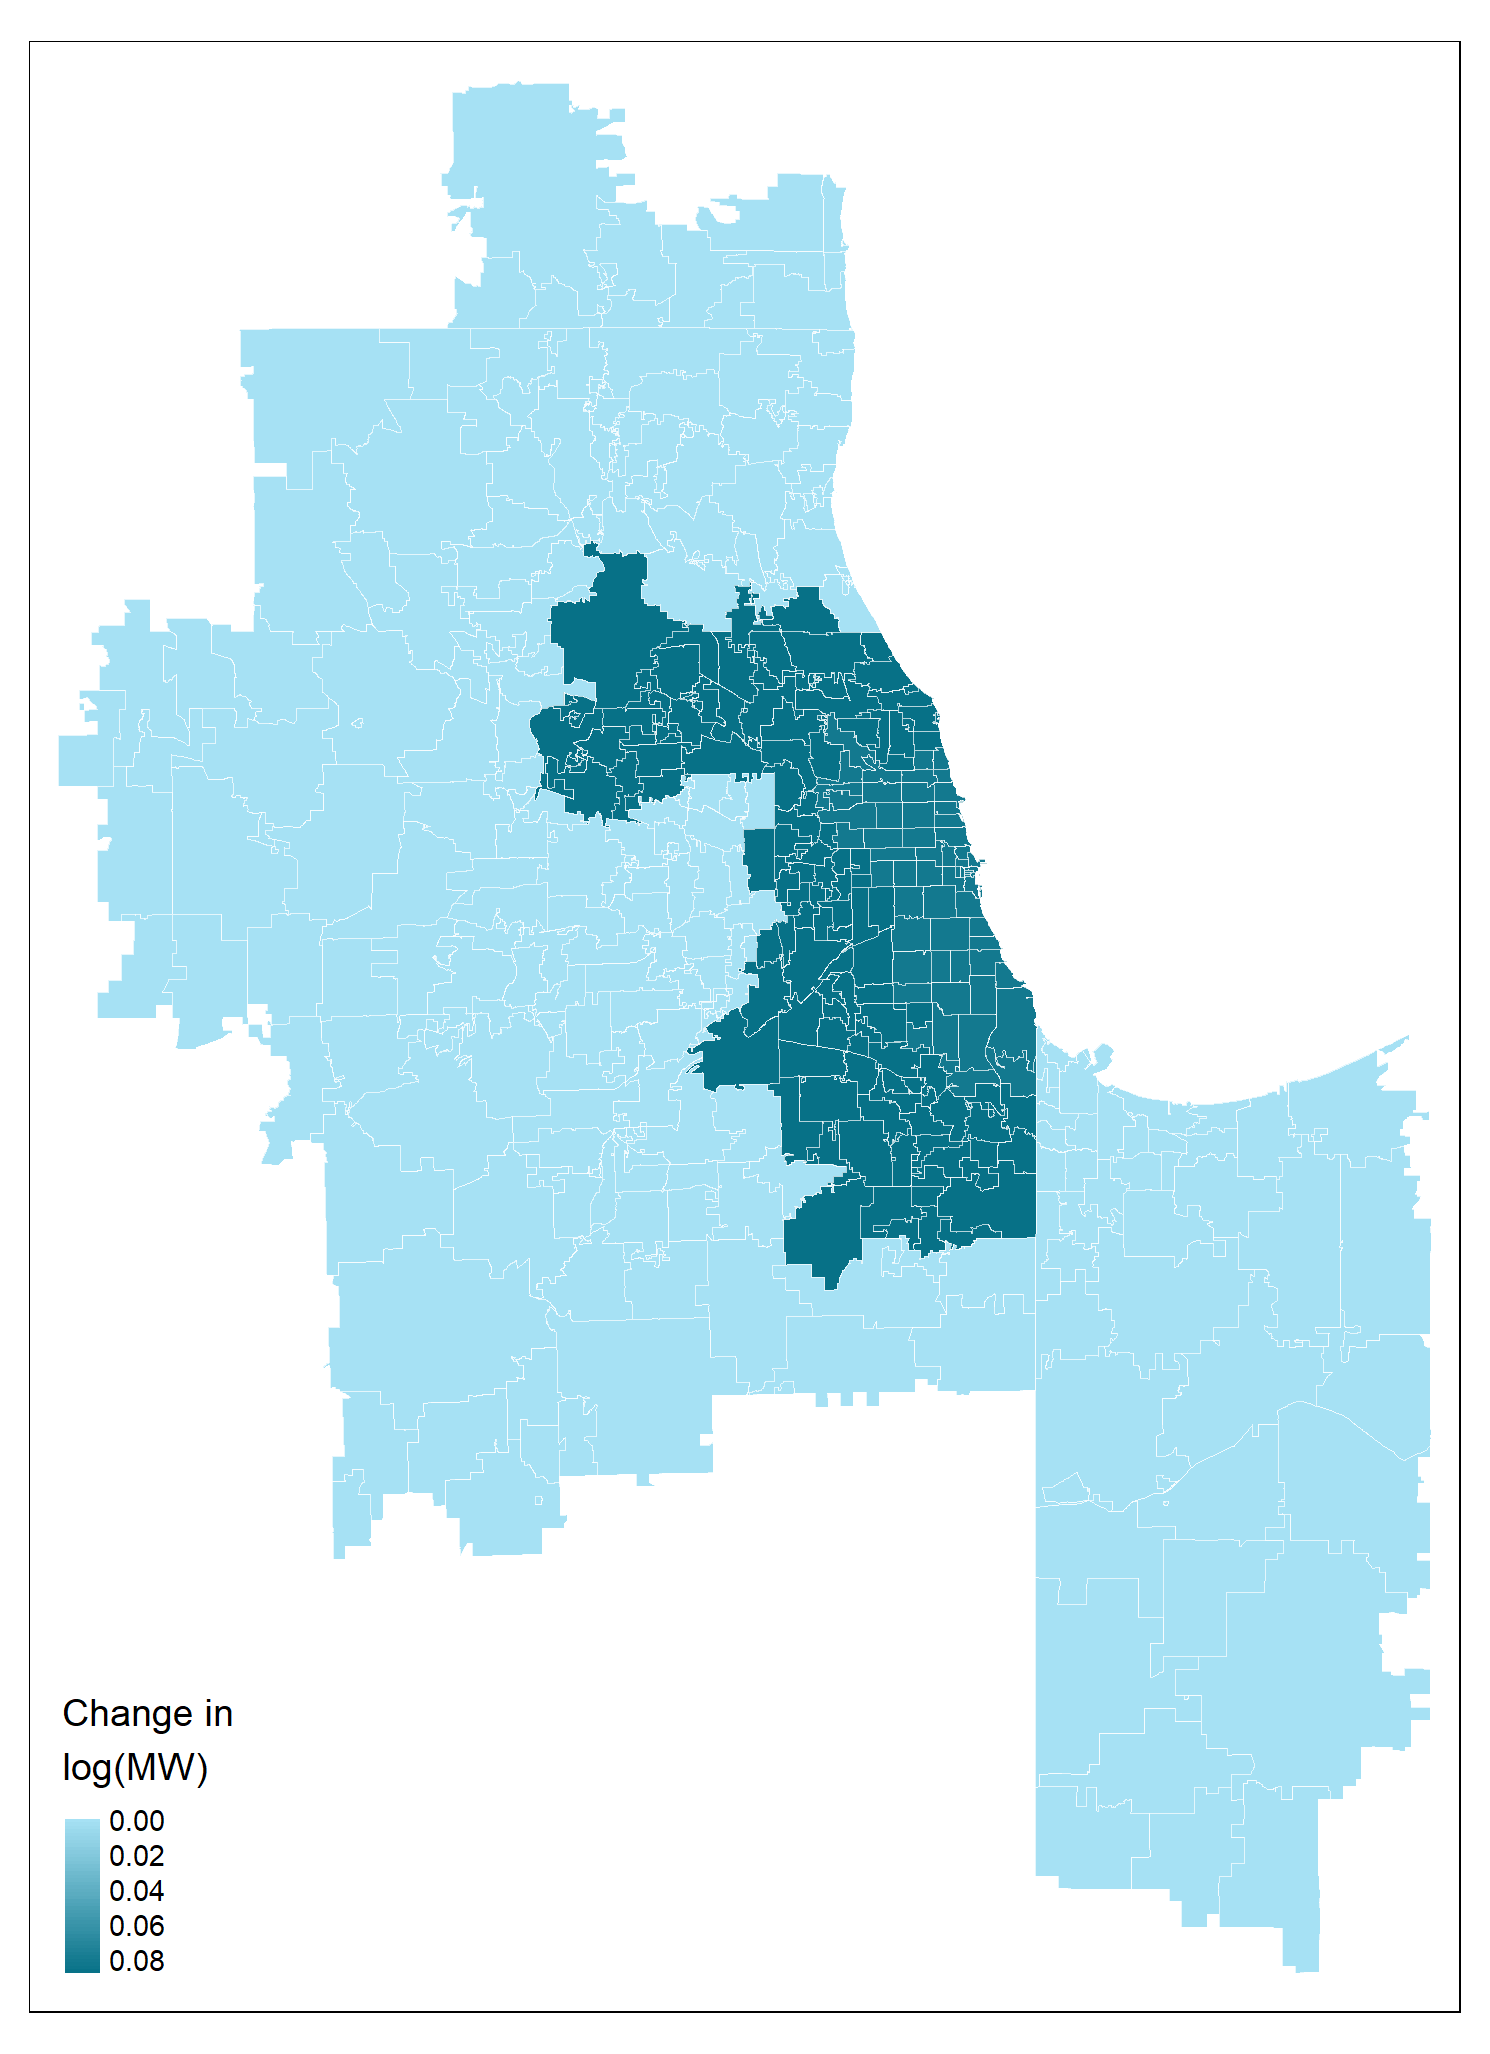
\includegraphics[scale = 0.38]{maps_events/output/chicago_2019-6_actual_mw.png}
            \end{figure}   
        \end{column}
        \begin{column}{0.56\textwidth}
			Cook County, IL
            \begin{itemize}
                \item Raised local MW from \$12 to \$13 in July 2019. 
				\item State MW is \$8.25 since 2010, and federal MW is \$7.25 since 2009.
                \vspace{2mm}
                \pause
                \item A (naive) regression model of rents on same-location MW imposes 
				that rents can only be affected in Cook County.
                \vspace{2mm}
                \pause
                \item However, workers in Cook County may live somewhere else. 
				$\to$ We must account for commuting structure!
            \end{itemize}
        \end{column}
    \end{columns}
\end{frame}

\begin{frame}
\frametitle{A novel model-based measure of exposure to minimum wages}

    For ZIP code $i$ and month $t$ we define it as:
	$$
	\underline{w}^{\text{wrk}}_{it} = 
	\sum_{z \in \Z(i)} \pi_{i z} \ln \underline{w}_{zt} \ ,
	$$
	%% IMPORTANT: We average the log of the MW! (Not log the average)
	\vspace{-2.5mm}
	where
	\vspace{1mm}
	\begin{itemize} \small
		\item $\Z(i)$ are workplace locations of $i$'s residents, and
		\item $\pi_{i z} = \frac{L_{i z}}{L_i}$ is the share of $i$'s residents who work 
		in $z$.
	\end{itemize}
\end{frame}

\begin{frame}[label = chi_example]
\frametitle{A motivating example (continuation)}
    \vspace{-6mm}
    \begin{columns}
        \begin{column}{0.50\textwidth}
            \vspace{-4mm}
            \begin{figure}
                \centering
                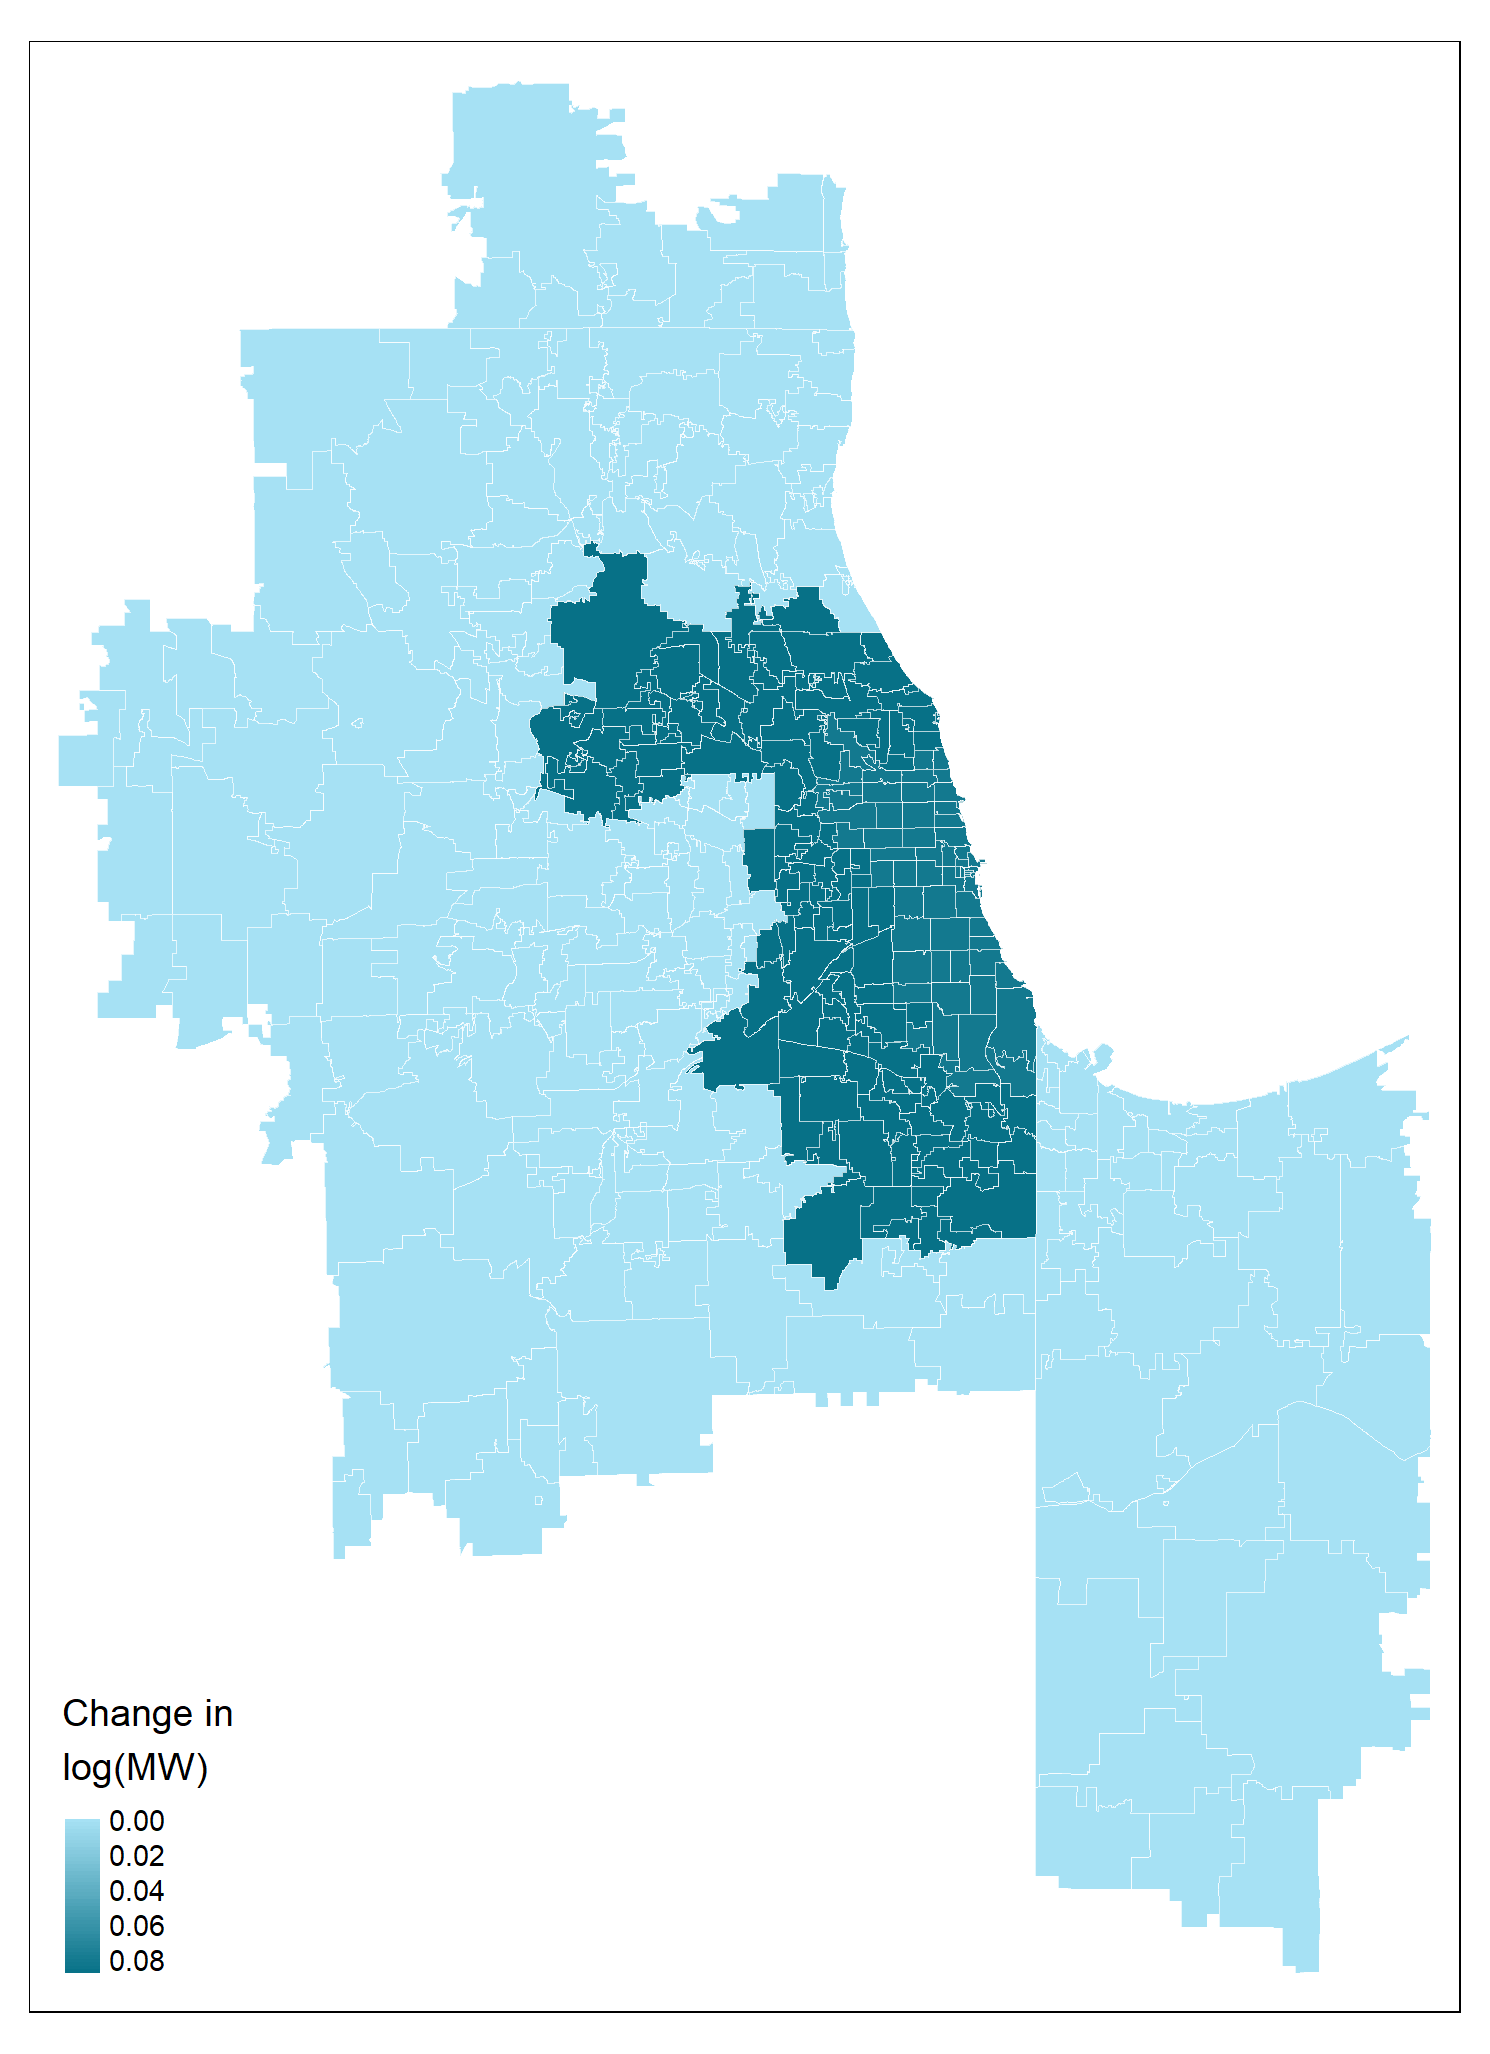
\includegraphics[scale = 0.36]{maps_events/output/chicago_2019-6_actual_mw.png}
            \end{figure}   
        \end{column}
        \begin{column}{0.50\textwidth}
            \vspace{-4mm}
            \begin{figure}
                \centering
                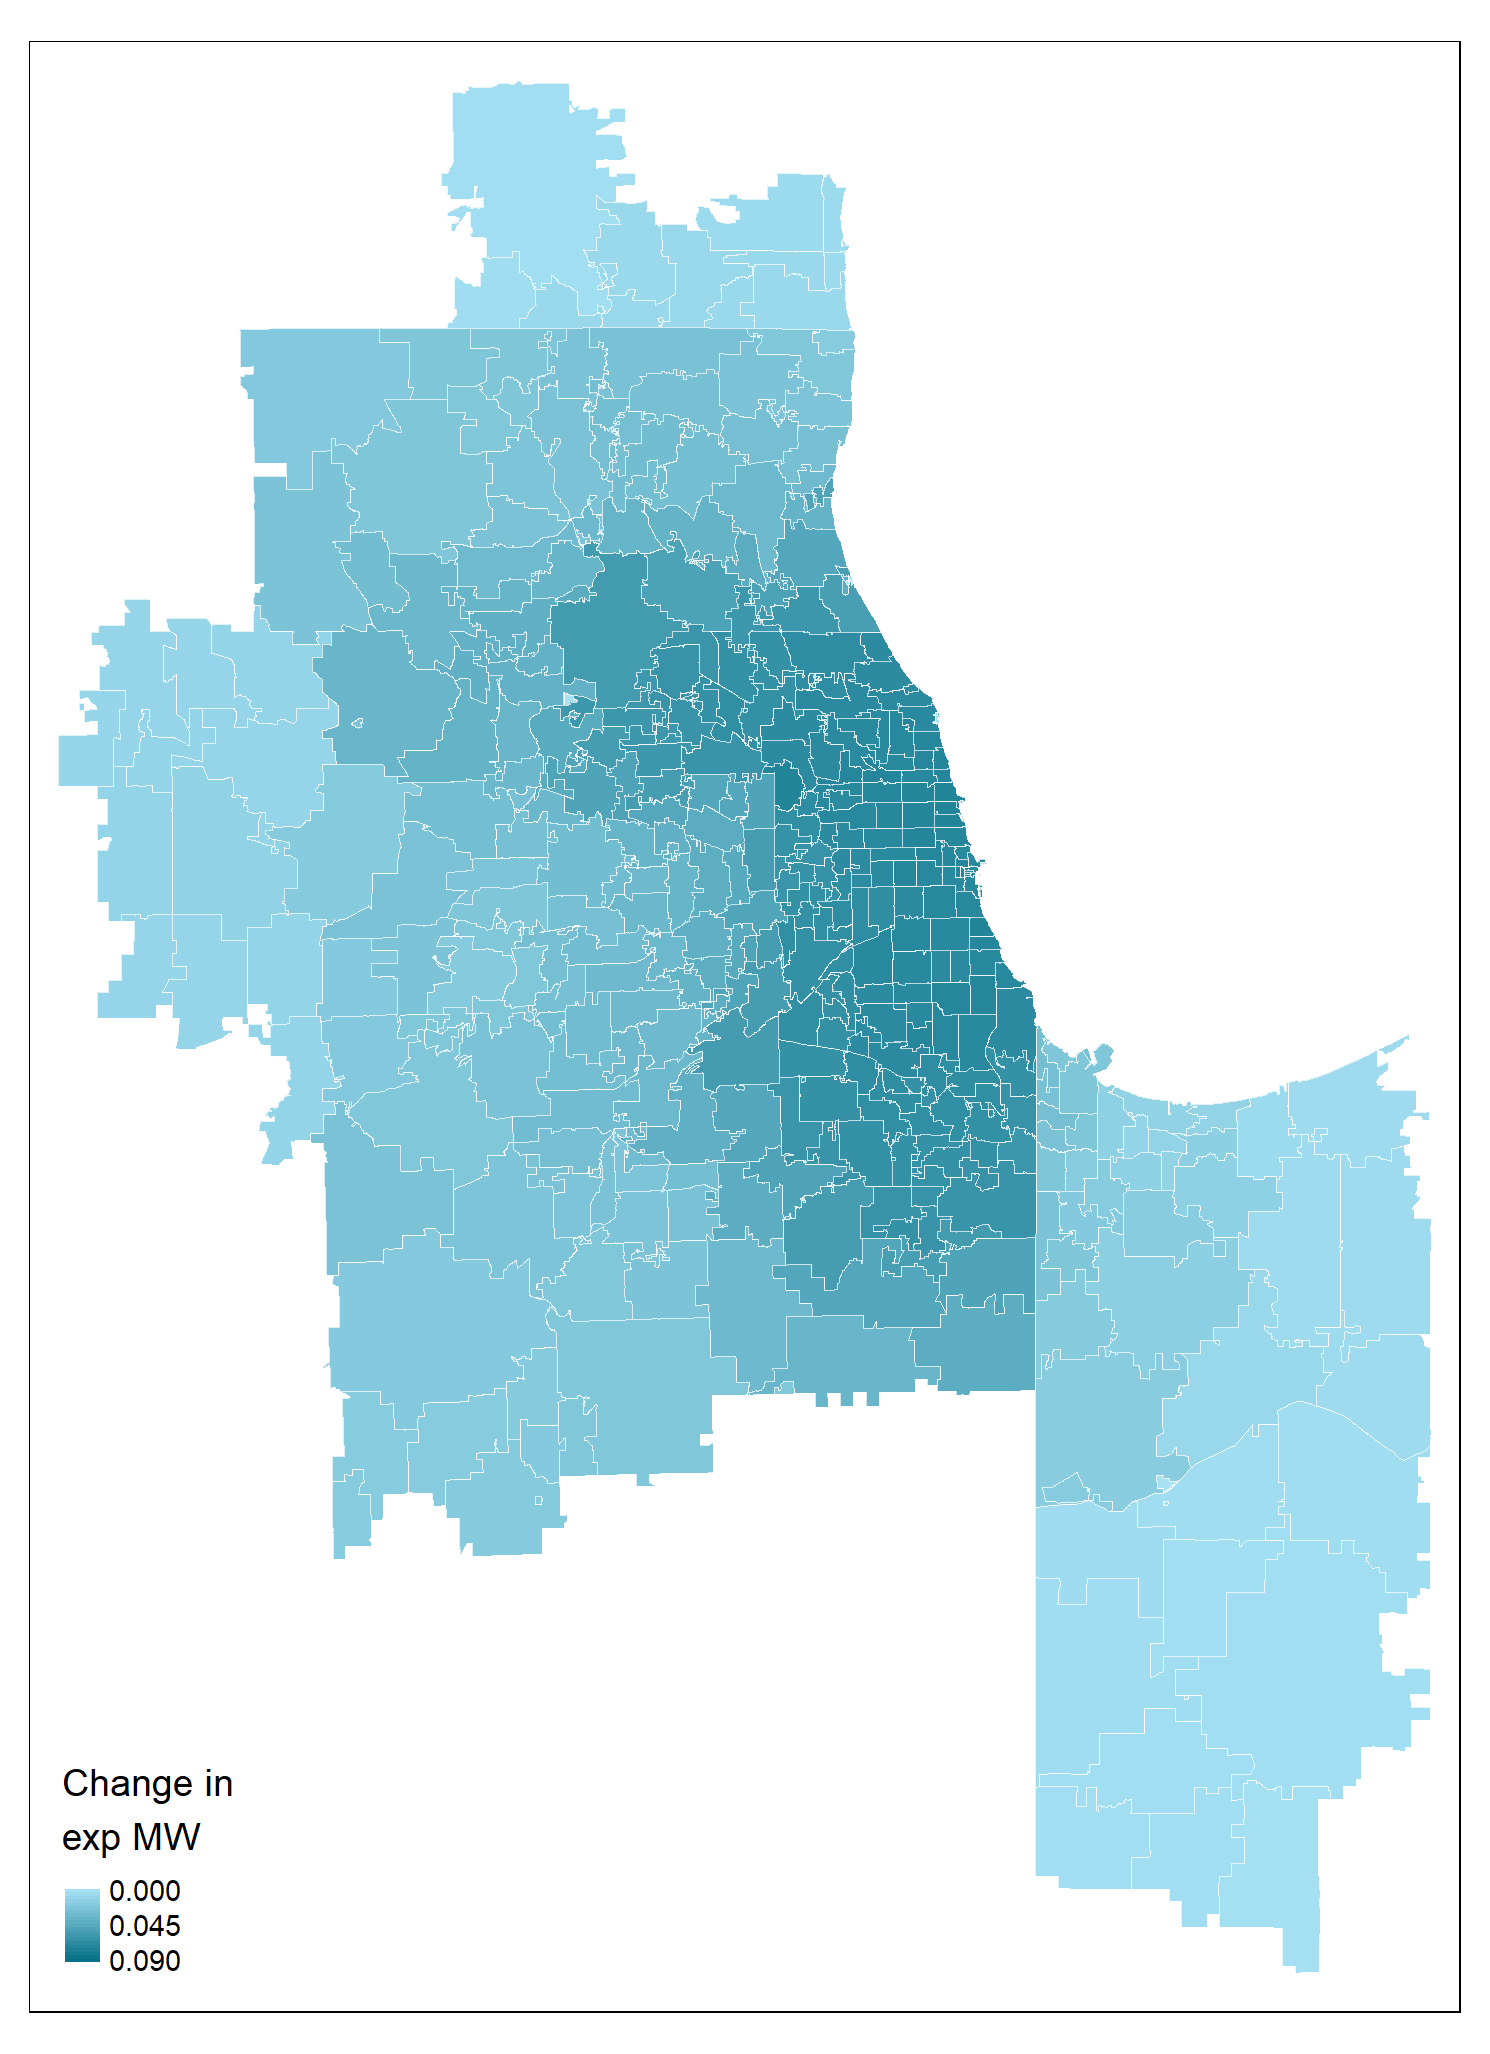
\includegraphics[scale = 0.36]{maps_events/output/chicago2019-6_exp_mw.png}
            \end{figure}   
        \end{column}
    \end{columns}
    \hspace{6mm}
    \hyperlink{nyc_example}{\beamerbutton{Example NYC}}    
    \hyperlink{seattle_example}{\beamerbutton{Example Seattle}}
    \hyperlink{bay_example}{\beamerbutton{Example Bay Area}}
    \hyperlink{san_diego_example}{\beamerbutton{Example San Diego}}
    \hyperlink{kc_example}{\beamerbutton{Example Kansas City}}
\end{frame}

\begin{frame}
	\frametitle{Outline for Today}
	\tableofcontents[hideallsubsections]
\end{frame}

\section{A Partial Equilibrium Model of Local Rental Markets}

\begin{frame}
    \frametitle{Overview}
    
    Goals of the model:
	\begin{itemize}
		\item Stylized answer to: what is the short-term effect of MW changes in rent prices?
		\item Motivate and derive a new measure of exposure to MW.
		\item Emphasize why residence and workerplace MWs may have different effects on the housing market.
		\item Motivate empirical strategy: use commuting patterns to account for spatial spillovers of MW policies.
	\end{itemize}
	
	\pause
	\vspace{2mm}
	The model is \textit{not} intended to:
	\begin{itemize}
		\item Describe within-city residential sorting.
		\item Describe local labor or goods markets.
		\item Perform general equilibrium welfare analysis of MW policies.
	\end{itemize}
\end{frame}

\begin{frame}
    \frametitle{Setup}
    
    Static rental market of some ZIP code $i$ embedded in a larger geography with finite
	set of ZIP codes $\Z$.    
    \begin{itemize}
		\vspace{2mm}
		\item Workers with residence $i$ may work in some other ZIP code $z\in\Z(i)\subseteq\Z$.

		\pause
		\vspace{2mm}
		\item Exogenous and fixed measure of $i$'s residents who work in $z$, $L_{iz}$.
		\begin{itemize}
			\item Residents in $i$: $L_i = \sum_{z \in \Z(i)} L_{iz}$.
			\item Workers in $z$: $L_z = \sum_{i \in \Z(i)} L_{iz}$.
		\end{itemize}
	
		\pause
		\vspace{2mm}
		\item Binding minimum wages: $\{\MW_i\}_{i\in\Z}$.
		
		\pause
		\vspace{2mm}
		\item $h_{i z} (R_i, \MW_i, \MW_z)$: housing demand of $i$'s residents that work in $z$, where $R_i$ 
		represents housing rents per square foot.

		\pause
		\vspace{2mm}
		\item $S_i \left(R_i \right)$: supply of square feet in $i$, which is increasing in $R_i$.

	\end{itemize}
\end{frame}

\begin{frame}
    \frametitle{Housing demand functions}
   
	\begin{assu}[Housing demand]\label{assu:housing_function}
		For all residence-workplace pairs, the housing demand functions $h_{iz} (R_i, \MW_i, \MW_z)$ is
		\begin{enumerate}
			\item continuously differentiable in its three arguments;
			\item decreasing in rental prices $R_i$;
			\item non-decreasing in workplace minimum wage $\MW_z$;
			\item non-increasing in residence minimum wage $\MW_i$.
		\end{enumerate}
		Furthermore, for at least one $z\in\Z(i)$, the inequalities in points (3)
		and (4) are strict.
	\end{assu}

	\pause 
	\vspace{2mm}

	\textbf{In words:} conditional on workplace MWs, residence MW may negatively affect disposable income
	and thus demand for housing.
\end{frame}

\begin{frame}[label = discuss4]
    \frametitle{Discussion on assumption 4}

	Evidence suggests that MW changes affect prices of local consumption
    \begin{itemize}
		\vspace{1mm}
        \item \textcite{MiyauchiEtAl2021} shows that individuals tend to consume close to home and that 
        they are aware of price differentials across neighborhoods.
		\vspace{1mm}
        \item MWs have been shown to increase prices of local consumption 
        \parencite[e.g.,][]{AllegrettoReich2018, Leung2021}.
    \end{itemize}

    \pause 
    \vspace{2mm}

    Will MW changes also affect housing demand? Consider an increase in residence MW:
    \begin{itemize}
		\vspace{1mm}
        \item If non-tradable goods use low-wage work as input, then local prices will increase.
		\vspace{1mm}
		\item Housing demand will fall if substitution effect is smaller than income effect.
		\begin{itemize}
			\item Sufficient condition: housing and local consumption are complements.
		\end{itemize}
    \end{itemize}

	Formalizing these ideas: \hyperlink{microfound}{\beamerbutton{Microfoundation}}  
\end{frame}

\begin{frame}
	\frametitle{Equilibrium}
	
	Define the housing demand in ZIP code $i$ as:
	
	 \[
	 H_{i} (R_i, \{\MW_z\}_{z\in\Z(i)}) = \sum_{z\in\Z(i)} L_{iz} h_{iz} (R_i, \MW_i, \MW_z)
	 \]
	
	The rental market of ZIP code $i$ is in equilibrium if
	
	$$ H_{i} (R_i, \{\MW_z\}_{z\in\Z(i)}) = S_i(R_i) $$
	
    Under suitable regularity conditions, the unique equilibrium is 
	$$R^*_i = f(\{\MW_i\}_{i\in\Z(i)})$$
	
	\vspace{3mm}
	\pause
	We are interested in the effects of MW policies on rents.
	\vspace{1mm}
	\begin{itemize} \small
		\item What is the effect of a change in the vector of MWs 
		$(\{d \MW_i\}_{i\in\Z(i)})'$ on equilibrium rents?
		\item Under what conditions can we represent those effects in a simpler way?
	\end{itemize}
\end{frame}

\begin{frame}[label = prop_comp_stat]
    \frametitle{Comparative Statics}
    
    \begin{prop}[Comparative Statics]\label{prop:comparative_statics}
        Under the assumptions of
        \begin{enumerate}
           \item fixed number of workers across workplace and residence pairs;
           \item housing demand equation satisfying conditions above; 
           \item continuously differentiable and increasing housing supply.
        \end{enumerate} 
        We have that
        \begin{itemize}
            \item workplace-MW hikes increase rents;
            \item holding constant workplace-MW hikes, residence-MW hikes decrease rents.
        \end{itemize}
    \end{prop}
\end{frame}

\begin{frame}[label = proof_comp_stat]
\frametitle{Proof of Proposition (Comparative Statics)}

    Fully differentiate the market clearing condition with respect to $\ln R_i$ and 
    $\ln \MW_i$ for all $i\in\Z(i)$ and re-arrange terms to get:
    \begin{equation}\label{eq:diff_equilibrium}
        \Big(\eta_i - \sum_z \pi_{iz} \xi_{iz} \Big) d \ln R_i
        = 
        \sum_z \pi_{iz} \left(\epsilon_{iz}^i d \ln \MW_i 
                            + \epsilon_{iz}^z d \ln \MW_z \right) ,
    \end{equation}
    where:
    \begin{itemize}
        \item $\eta_i = \frac{1}{L_i} \frac{d S_i}{d R_i} \frac{R_i}{S_i}$ is the per resident elasticity 
        of housing supply in $i$
        \item Commuter shares: $\pi_{iz} = \frac{L_{iz}}{L_i}$
        \item $\xi_{iz} = \frac{d h_{iz}}{d R_i} \frac{R_i}{\sum_z \pi_{iz} h_{iz}}$ is the 
        elasticity of housing demand to rents at average per-capita demand of $i$
        \item  $\epsilon_{iz}^i = \frac{d h_{iz}}{d \MW_i} \frac{\MW_i}{\sum_z \pi_{iz} h_{iz}}$ and 
        $\epsilon_{iz}^z = \frac{d h_{iz}}{d \MW_z} \frac{\MW_z}{\sum_z \pi_{iz} h_{iz}}$ 
        are the elasticities of housing demand to workplace and residence MWs also at
         the average per-capita demand of $i$
    \end{itemize}
\end{frame}

\begin{frame}
    \frametitle{Proof of Proposition (Comparative Statics) (continuation)}
    
    Using assumption on housing demand we have that
    $$
	\xi_{iz} < 0, \quad\quad\quad \epsilon_{iz}^i < 0, \quad\quad\quad \epsilon_{iz}^z > 0 .
	$$
	\vspace{1mm}
    Therefore, it follows from \eqref{eq:diff_equilibrium} that
    \begin{enumerate}
        \item an increase in workplace MW unambiguously increases rents;
        \item an increase in residence MW on rents is generally ambiguous 
        (as long as some residents of $i$ also work in $i$) as it is composed of a direct negative 
        effect and an indirect positive effect through workplace MW;\footnote{The sign of the overall partial effect depends on the sign of 
    $\pi_{ii} \epsilon_{ii}^z + \sum_z \pi_{iz} \epsilon_{iz}^i$.}
        \item Holding constant workplace MWs, the effect of the residence MW is negative.
    \end{enumerate}    
\end{frame}

\begin{frame}[label = representation_prop]
    \frametitle{Simplifying the equilibrium rents function}
    
	\begin{prop}[Representation]\label{prop:representation}
		Under the assumption of constant elasticity of housing demand (across workplace locations)
		to workplace minimum wages we have that:
		\begin{itemize}
			\item We can write the change in \textbf{log rents} as a function of the change in two 
			MW-based measures: the \textbf{workplace log MW} and the \textbf{residence log MW}.
		\end{itemize}
	\end{prop}

	\pause
	\vspace{2mm}

	\begin{proof}
		Set $\epsilon_{iz}^z = \epsilon_i^z$ for all $z\in\Z(i)$ 
		we can manipulate \eqref{eq:diff_equilibrium} to write:
		\begin{equation} \label{eq:theory_represenation}
			\underbrace{d \ln R_i}_{dr_i} 
			    = \beta_i \underbrace{\sum_i \pi_{iz} d\ln \MW_z}_{d\MW^{\text{wrk}}_{i}}
				+ \gamma_i \underbrace{d \ln \MW_i}_{d\MW^{\text{res}}_{i}}
		\end{equation}
		where $\beta_i = \frac{\epsilon_{i}^z}{\eta_{i} - \sum_z \pi_{iz} \xi_{iz}}$ 
		and $\gamma_i = \frac{\sum_z \pi_{iz} \epsilon_{iz}^i}{\eta_{i} - \sum_z \pi_{iz} \xi_{iz}}$.
	\end{proof}
\end{frame}

\begin{frame}
	\frametitle{Motivating our empirical strategy}
	We have that the theoretical partial equilibrium effect of a change in elements of a vector of MW on rents is given by:
		\begin{equation}
				d r_i = \beta_i d \MW^{\text{wrk}}_{i}+ \gamma_i d \MW^{\text{res}}_i
			\end{equation}
			
	Where, because of Proposition (Comparative Statics), we have that:
	\begin{itemize}
		\item The partial effect of workplace MW, $\beta_i = \frac{\epsilon_{i}^z}{\eta_{i} - \sum_z \pi_{iz} \xi_{iz}} > 0$;
		\item The partial effect of residence MW, $\gamma_i = \frac{\sum_z \pi_{iz} \epsilon_{iz}^i}{\eta_{i} 
				- \sum_z \pi_{iz} \xi_{iz}} < 0$.
	\end{itemize}

	\pause
	\vspace{2mm}
	Today, we will estimate an empirical analog assuming homogenous effects across 
	locations.

\end{frame}


\section{Data}

\begin{frame}[label = zillow_data]
	\frametitle{Zillow Data}
	
	\begin{itemize}
		\item Leader online real estate and rental platform in the U.S. {\small (more 
		than 110 million homes and 170 million unique monthly users in 2019).}
		
		\vspace{2mm} \item
		Provides \textit{median} rents data at ZIP code, county, and state levels 
		at a monthly frequency for several housing categories.
		
		\pause
		\vspace{2mm} \item
		We use category single-family, condominium, and cooperative houses (SFCC):
		\begin{itemize}
			\item Most common housing type in the U.S.
			\item Most populated series in Zillow.
			%%\item Captures trends in metropolitan housing markets. 

		\end{itemize}
		\hyperlink{zillow_safmr}{\beamerbutton{Comparison with Small Area Fair Market Rents}}
		
		\pause
		\vspace{2mm} \item
		Limitation: Zillow sample is not random.
		
		\hyperlink{zillow_pop_density}{\beamerbutton{Zillow ZIP Codes and Population Density}}

	\end{itemize}
\end{frame}

\begin{frame}[label=stat_MW]
	\frametitle{The Statutory MW}
	
	\begin{itemize}
		\item
		Collect MW data at state, county and city levels between Jan 2010 and Dec 2019.
		\begin{itemize}
		    \item Up to 2016 we relied on data from \cite{CegnizEtAl2019} and \cite{VaghulZIPperer2016} 
		\end{itemize}
		
		\vspace{2mm} \item
		For each US Postal ZIP Code we assigned place, ZCTA, city, county, and state codes. 
						
		\vspace{2mm} \item
		Define statutory MW in ZIP code as maximum between state and local levels.
		
		\pause
		\vspace{2mm} \item
		ZIP codes available in Zillow contain 18,689 changes at the ZIP code-month level.
		\vspace{-3.5mm} 
		\begin{itemize} \small
			\item 151 state-level changes.
			\item 182 county and city-level changes.
		\end{itemize}
		%% We use 4,224 events at the ZIP code-month level in our estimating panel
		 
		\hyperlink{dist_mw_changes}{\beamerbutton{Distribution of MW changes}}

	\end{itemize}
	
\end{frame}

\subsection{Commuting shares}

\begin{frame}
	\frametitle{Using LODES to construct the experienced log MW}
	
	\vspace{2mm}
	
	Construct \textbf{origin-destination matrix} at ZIP code level from LODES 2009 to 2018.
	%% Original data comes at the block-group level
	
	\vspace{2mm}

	We observe:
	\begin{itemize} \small
		\item Number of workers residing in a ZIP code and working in every other 
		ZIP code.
		\item Analogous, matrix for number of workers younger than 29 and earning less than 
		\$1,251.
	\end{itemize}
	
	\vspace{2mm}	
	In our baseline specification we use constant commuter shares from 2017.
	\begin{itemize} \small
		\item Results are robust to using other years and groups.
	\end{itemize}
\end{frame}

\subsection{Other Data sources}

\begin{frame}
	\frametitle{Other Data Sources} 
	
	\begin{itemize}
		\item Economic controls from Quarterly Census of Employment and Wages 
		{\small (QCEW)}.
		\vspace{2mm} \item IRS Statistics of income - ZIP Code Aggregates
		\vspace{2mm} \item American Community Survey
		\vspace{2mm} \item US Census
		\vspace{2mm} \item Shapefile of US Postal ZIP Codes
	\end{itemize}
\end{frame}

\section{Empirical Strategy}

\begin{frame}[label = stat_only_model]
	\frametitle{Empirical (Naive) model}
	
	One may estimate the following first differences model:
	
	$$
	\Delta r_{it} = \tilde\delta_t + 
	\tilde\beta {\color{blue} \Delta \MW^{\text{res}}_{it}} + 
	\Delta \mathbf{X}^{'}_{c(i)t} \tilde\eta + 
	\Delta \tilde\varepsilon_{it} ,
	$$
	
	where	
	\begin{itemize} \small
	\item ZIP code $i$, county $c(i)$, month $t$.
	
	\item \vspace{1mm} $r_{it} = \ln R_{it}$: log of rents per square foot.
	
	\item \vspace{1mm} ${\color{blue} \MW^{\text{res}}_{it}} = \ln \MW_{it}$: log of the residence MW.
	
	\item \vspace{1mm} $\tilde\delta_t$: month fixed effects (ZIP code FE $\tilde\alpha_i 
	$ is 
	implicit).
	
	\item \vspace{.5mm} $\mathbf{X}_{c(i)t}$: time-varying controls at the county level.
	\end{itemize}
\end{frame}

\begin{frame}
	\frametitle{Empirical model}
		
	Now add experienced MW:
	$$
	\Delta r_{it} = \delta_t +
	    \beta {\color{red}\Delta \MW^{\text{wrk}}_{it}} +
		\gamma {\color{blue} \Delta \MW^{\text{res}}_{it}} + 
		\Delta \mathbf{X}^{'}_{c(i)t} \eta + 
		\Delta \varepsilon_{it} ,
	$$
	
	where 
	\[
	{\color{red} \MW^{\text{wrk}}_{it}} = 
		\sum_{z \in \Z(i)} \pi_{i z} \ln \underline{w}_{zt}
	\] 
	
	is our measure of access to MW in workplace locations derived from the model.


	\pause
	\vspace{2mm}
	For causal effect of $\beta$ we need:
	$$
	E \left[\Delta \varepsilon_{ict} {\color{red} \Delta 
	\MW^{\text{wrk}}_{i\tau}} 
	\big| {\color{blue}\Delta \MW^{\text{res}}_{it}}, \delta_t, \Delta 
	\mathbf{X}_{c(i)t} \right] = 0
	\quad \quad \forall \tau \in \left[ \underline{T}, \overline{T} \right]
	$$
	
	\pause
	\vspace{2mm}
	\textbf{In words}: conditional on FEs, controls, and {\color{blue} MW in same ZIP 
	code}, unobserved innovations to rent shocks are uncorrelated with past and future 
	values of log MW changes {\color{red} in nearby ZIP codes}.
\end{frame}

\begin{frame}
	\frametitle{Discussion Identification Assumption}
	
	Thus, for causal effect of $\beta$ we need:
	$$
	E \left[\Delta \varepsilon_{it} \Delta \MW^{\text{wrk}}_{it}  
	\big| \Delta \MW^{\text{res}}_{it}, \delta_t, \Delta 
	\mathbf{X}_{c(i)t} \right] = 0
	\quad \quad \forall \tau \in \left[ \underline{T}, \overline{T} \right]
	$$
	\vspace{.5mm}
	Analogously, for causal effect of $\gamma$ we need:
	$$
	E \left[\Delta \varepsilon_{it} \Delta \MW^{\text{res}}_{it}  
	\big| \Delta \MW^{\text{wrk}}_{it}, \delta_t, \Delta \mathbf{X}_{c(i)t} 
	\right] = 0
	\quad \quad \forall \tau \in \left[ \underline{T}, \overline{T} \right]
	$$
	
	\pause
	\vspace{.5mm}
	\textbf{Is this plausible?}
	\begin{itemize} \small
		\vspace{.5mm}
		\item MW policies are rarely set by considering differential dynamics of the 
		rental housing market within metropolitan areas.
		%% For example, the Congressional Budget Office (CBO) doesn't mention rents even 
		%% once in it's study of the effects of the Wage Act of 2021
		%% https://www.cbo.gov/system/files/2021-02/56975-Minimum-Wage.pdf
		
		\vspace{.5mm}
		\item Furthermore, there is substantial heterogeneity in the housing market 
		across ZIP codes.
		
		\vspace{.5mm}
		\item Indirectly test assumption through pre-trends, assuming no anticipatory 
		effects in housing market.
	\end{itemize}
\end{frame}


\begin{frame}[label = dyn_model]
	\frametitle{Testing Identification with a Dynamic model}
	
	Adding leads and lags of the experienced log MW:
	
	$$
	\Delta r_{it} = \delta_t
		+ \sum_{r=-s}^{s} \beta_r \Delta \MW^{\text{exp}}_{i,t+r}
		+ \gamma \Delta \MW^{\text{res}}_{it}
		+ \Delta \mathbf{X}^{'}_{c(i)t}\eta
		+ \Delta \varepsilon_{it}
    $$	
	where $\{\beta_r\}_{r=-s}^{s}$ are the dynamic coefficients.
	
	\vspace{3mm}

    Analogously, one can add instead the leads and lags of the log residence MW
    to test the identification assumption of $\gamma$.
\end{frame}

\begin{frame}
	\frametitle{Potential Outcomes with Continuous Treatment and Spatial Spillovers}
	Consider the potential outcomes model for log rents given by:

	\[
	r_{it}=r_{it}\left(\{\underline{w}_{zt}\}_{z\in\Z(i)}\right)
	\]

	We impose some structure by assuming that:

	\[
	r_{it}(\underline{w}_{1t},...,\underline{w}_{it}, ..., \underline{w}_{Z_{\Z(i)}}) = \alpha_{i} + 
	\delta_{t} + \beta \underbrace{\sum_{z\in\Z(i)}\pi_{iz}\ln \underline{w}_{zt}}_{\MW^{\text{wrk}}_{it}} +
	\gamma \underbrace{\ln \underline{w}_{it}}_{\MW^{\text{res}}_{it}} + u_{it}
	\]
	where the econometrician has knowledge of the commuting shares, and $u_{it}$ is an unobserved shock.

	\pause 

	\vspace{2mm}

	\textbf{Questions:} 
	\begin{itemize}
		\item Are $\beta$ and $\gamma$ identified? 
		\item Through which comparisons? 
	\end{itemize}
\end{frame}

\begin{frame}
	\frametitle{A simple example with 3 ZIP Codes and 2 time periods}

	Consider a hypothetical metropolitan area
	\begin{itemize}
		\item 3 ZIP Codes and 2 consecutive periods (periods 0 and 1)
		\item In $t=0$ the MW is \$0 everywhere, but in $t=1$ the MW in unit 2 increases to \$1
	\end{itemize}

	\pause 
	\vspace{2mm}
	We have have 6 observations for rents, and the potential outcomes model implies:
	\begin{itemize}
		\item $r_{10}(0,0,0)=\alpha_{1}+\delta_{0}+u_{10}$
		\item $r_{11}(0,1,0)=\alpha_{1}+\delta_{1}+\beta\pi_{12}+u_{11}$
		\item $r_{20}(0,0,0)=\alpha_{2}+\delta_{0}+u_{20}$
		\item $r_{21}(0,1,0)=\alpha_{2}+\delta_{1}+\gamma+\beta\pi_{22}+u_{21}$
		\item $r_{30}(0,0,0)=\alpha_{3}+\delta_{0}+u_{30}$
		\item $r_{31}(0,1,0)=\alpha_{3}+\delta_{1}+\beta\pi_{32}+u_{31}$
	\end{itemize}
\end{frame}

\begin{frame}
	\frametitle{Solving for $\beta$}

	Taking time differences, and denoting $\Delta x_i = x_{i1} - r_{i0}$ and $\delta = \delta_{1} - \delta_{0}$ we have that:

	\begin{itemize}
		\item $\Delta r_{1} = \delta + \beta\pi_{12} + \Delta u_{1}f$
		\item $\Delta r_{2} = \delta + \gamma + \beta\pi_{22} + \Delta u_{2}$
		\item $\Delta r_{3} = \delta + \beta\pi_{32} + \Delta u_{3}$
	\end{itemize}

	\pause
	\vspace{2mm}

	Now differentiate the indirectly treated units and rearrange to obtain:
	\[
	\beta = \frac{(\Delta r_{3} - \Delta r_{1}) + (\Delta u_{3} - \Delta u_{1})}{\pi_{32} - \pi_{12}}
	\]

	\vspace{2mm}
	To identify $\beta$ we need:
	\begin{itemize}
		\item parallel trends across indirectly treated units: $\Delta u_{3} - \Delta u_{1} = 0$
		\item variation in exposure across indirectly treated units:  $\pi_{32} - \pi_{12} \neq 0$
	\end{itemize}
\end{frame}

\begin{frame}
	\frametitle{Solving for $\gamma$}

	Differentiate the treated unit with an indirectly treated unit and rearrange to obtain:
	\[
	\begin{split}
	\gamma & = \Delta r_{2} - \Delta r_{1} - \beta(\pi_{22} - \pi_{12}) + (\Delta u_{2} - \Delta u_{1}) \\
		& = \Delta r_{2} - \left[\frac{\pi_{32} - \pi_{22}}{\pi_{32} - \pi_{12}}\Delta r_{1} + \frac{\pi_{12} - 
		\pi_{22}}{\pi_{32} - \pi_{12}}\Delta r_{3}\right] + (\Delta u_{2} - \Delta u_{1})
	\end{split}
	\]

	\vspace{2mm}
	To additionally identify $\gamma$ we need
	\begin{itemize}
		\item parallel trends across treated and indirectly treated units: $\Delta u_{2} - \Delta u_{1} = 0$
	\end{itemize}
\end{frame}

\begin{frame}
\frametitle{Interpretation}

	\vspace{2mm}

	\begin{itemize}
		\vspace{2mm}\item We need parallel trends across treated and indirectly treated groups. 
		\vspace{2mm}\item Interestingly, with continuous treatment and an assumption of how spillovers are dosed, 
		we don't need pure control control units, as we can make contrasts of units with different exposure levels. 
		\vspace{2mm}\item $\beta$ can be thought of a difference-in-differences between indirectly treated units
		adjusted by their difference in exposure to the treated units. 
		\vspace{2mm}\item $\gamma$ is identified by a difference-in-differences in which we difference the treated units with a linear combination 
		of the difference in indirectly treated units, where the coefficients reflect the relative difference of exposure to treated units.
	\end{itemize}
\end{frame}

\section{Results}

\subsection{Main Results}

\begin{frame}[label = static_tab]
    \frametitle{Static Model}

    \begin{table}
    \label{tab:static}
    \scalebox{0.8}{
        \begin{tabular}{l*{4}{c}}
            \toprule
            & \multicolumn{1}{c}{\shortstack{Change wkp.\ MW\\$\Delta\mw_{it}^{\wkp}$}}
                & \multicolumn{3}{c}{\shortstack{Change log rents\\$\Delta r_{it}$}} \\ \cmidrule(lr){2-2}\cmidrule(lr){3-5}
                                               & (1)   & (2)   & (3)   & (4)            \\ \midrule
            Change residence MW 
                      $\Delta\mw_{it}^{\res}$  &  #4#  &  #4#  &       &  #4#     \\
                                               & (#4#) & (#4#) &       & (#4#)    \\
            Change workplace MW 
                       $\Delta\mw_{it}^{\wkp}$ &       &       &  #4#  & #4#      \\
                                               &       &       & (#4#) & (#4#)    \\ \midrule
            Sum of coefficients                &       &       &       &  #4#     \\
                                               &       &       &       & (#4#)    \\ \midrule
            County-quarter economic controls   &  Yes  & Yes   & Yes   & Yes      \\
            P-value equality                   &       &       &       & #4#      \\
            R-squared                          &  #4#  &  #4#  &  #4#  & #4#      \\
            Observations                       & #0,#  & #0,#  & #0,#  & #0,#     \\\bottomrule
        \end{tabular}
    }
\end{table}

    \hyperlink{example_pred_chi_07_2019}{\beamerbutton{Example Predictions for Chicago July 2019}}
\end{frame}

\begin{frame}[label = dyn_baseline_plot]
	\frametitle{Including leads and lags of workplace MW}

	\begin{figure}
		\centering
		\vspace{-2mm}
		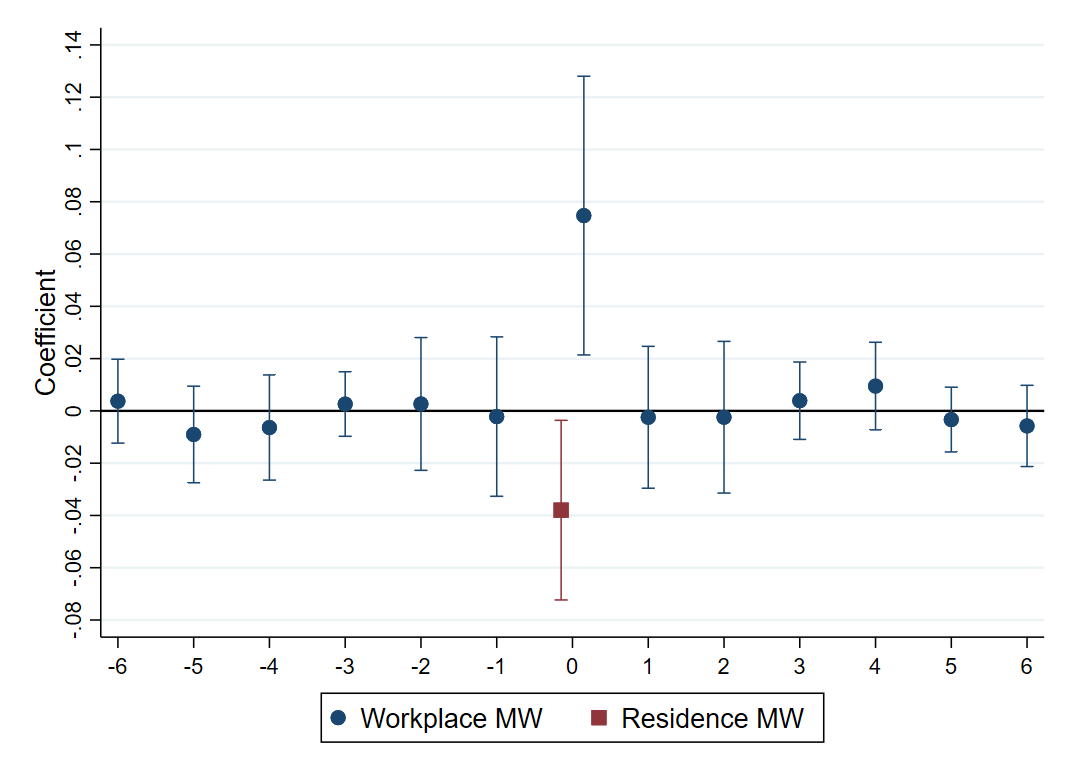
\includegraphics[width=0.70\textwidth]{fd_baseline/output/fd_baseline_exp_ln_mw_17_dynamic.png}
	\end{figure}

	\hyperlink{dynamic_mw}{\beamerbutton{Leads and Lags of Residence MW}}
	\hyperlink{fd_both_dynamic}{\beamerbutton{Leads and Lags of Both Residence and Workplace MW}}

	
\end{frame}

\begin{frame}[label = robus_sample]
	\frametitle{Robustness checks and Sample Selection}

	Concerns about differential geographic trends across treated
	\begin{itemize}
		\item Inclusion of non-parametric geographical trends
		\item Inclusion of ZIP code-specific parametric trends
		\item Use only MW changes that are not pre-announced (work in progress)
		\item Stack events a lá \cite{CegnizEtAl2019} (work in progress)
	\end{itemize}
	\hyperlink{robustness_geo}{\beamerbutton{Robustness results}}

	\vspace{3mm}
	Concerns that results are particular to our sample or not generalizable
	\begin{itemize}
		\item Estimate model on fully balanced and unbalanced panels
		\item Reweight observations to match characteristics of average urban ZIP code
	\end{itemize}
	\hyperlink{robustness_geo}{\beamerbutton{Sample-issues results}}
	
	\vspace{3mm}
	Concerns about workplace MW definition:
	\begin{itemize}
		\item Estimate under different commuter shares.
	\end{itemize}
	\hyperlink{robustness_exp_mw}{\beamerbutton{Sensitivity to alternative commuter shares}}
\end{frame}

\section{The incidence of a counterfactual federal MW change}

\begin{frame}
    \frametitle{Overview}
    
    Entire commuting structure determines the incidence of MW policies.
    \begin{itemize}
    	\vspace{1mm}
    	\item In some ZIP codes both residence and workplace MW increase
    	\vspace{1mm}
    	\item Other nearby ZIP codes are affected only through workplace
    \end{itemize}
    
    \pause
    \vspace{3mm}
    Consider an increase of the federal MW to \$9 in January 2020.
    \begin{itemize}
    	\vspace{1mm}
    	\item Changes income $\{\Delta Y_i\}_{i\in\Z}$ and housing expenditure $\{\Delta H_i\}_{i\in\Z}$
    \end{itemize}
    
    \pause
    \vspace{3mm}
    How much out of each extra dollar is captured by landlords?
   
\end{frame}

\begin{frame}
	\frametitle{Pass-through coefficients}

	Define pass-through coefficients as	
	\begin{equation*}
		\rho_i := \frac{\Delta H_i}{\Delta Y_i} =  \frac{h^{\text{Post}}_i R^{\text{Post}}_i - h^{\text{Pre}}_i R^{\text{Pre}}_i}{\Delta Y_i}
	\end{equation*}
	where 
	\begin{itemize}
		\item $h$ denotes rented space in $i$ (square feet)
		\item Pre and Post indicate moments before and after the increase
	\end{itemize}

	\pause
	\vspace{3mm}
	Change in rented space are unobserved. We assume $h^{\text{Pre}}_i = h^{\text{Post}}_i = h_i$ so
	\begin{equation*}
		\rho_i = \frac{h^{\text{Post}}_i R^{\text{Post}}_i - h^{\text{Pre}}_i R^{\text{Pre}}_i}{\Delta Y_i} = h_i \frac{\Delta R_i}{\Delta Y_i}
	\end{equation*}
	If $\Delta h_i > 0$ then our estimate of $\rho_i$ is a lower bound.

\end{frame}

\begin{frame}
	\frametitle{Pass-through under the model}

	According to the model,
	$$
	\Delta \ln R_i = \beta \MW_i^{\text{wkr}} + \gamma \MW_i^{\text{res}}
	$$
	We also define
	$$
	\Delta \ln Y_i = \varepsilon \MW_i^{\text{wkr}}
	$$

	\pause
	\vspace{2mm}
	Algebra implies
	\begin{equation*}
		\begin{split}
			\rho_i & = h_i \left[ 
				\frac{\exp \left(\Delta \ln R_i + \ln R_i \right) - R_i }{\exp \left( \Delta \ln Y_i + \ln Y_i \right) - Y_i }
				\right] \\
				& = \alpha_i \left[
					\frac{\exp \left( \beta \MW_i^{\text{wkr}} + \gamma \MW_i^{\text{res}} \right) - 1 }{\exp \left( \varepsilon \MW_i^{\text{wkr}} \right) - 1 }
				\right]
		\end{split}
	\end{equation*}
	where
	\begin{itemize}
		\item $\alpha_i = \frac{h_i R_i}{Y_i}$ is the share of $i$'s expenditure in housing
	\end{itemize}

	\vspace{2mm}
	We use our estimates to compute $\rho_i$ for urban ZIP codes.
	%% URBAN ZIP codes according to who? KNOW THIS
\end{frame}

\begin{frame}
	\frametitle{Increases in residence and workplace MWs}
	\begin{figure}
		\begin{subfigure}{0.51\textwidth}
			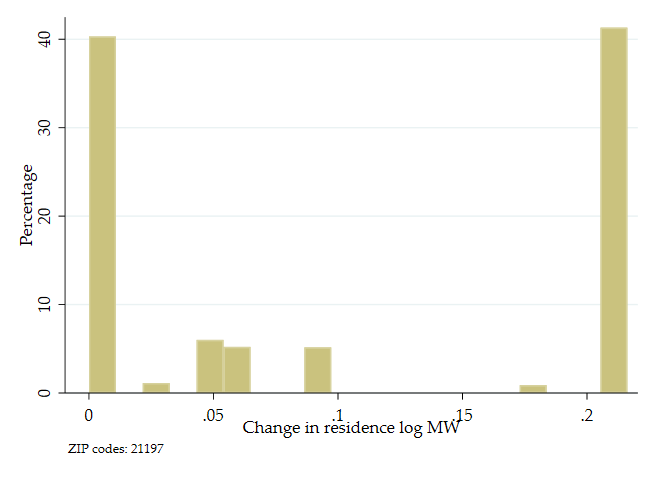
\includegraphics[width = 0.99\textwidth]{counterfactuals/output/d_ln_mw.png}
			\caption*{Residence MW}
		\end{subfigure}%
		\begin{subfigure}{0.51\textwidth}
			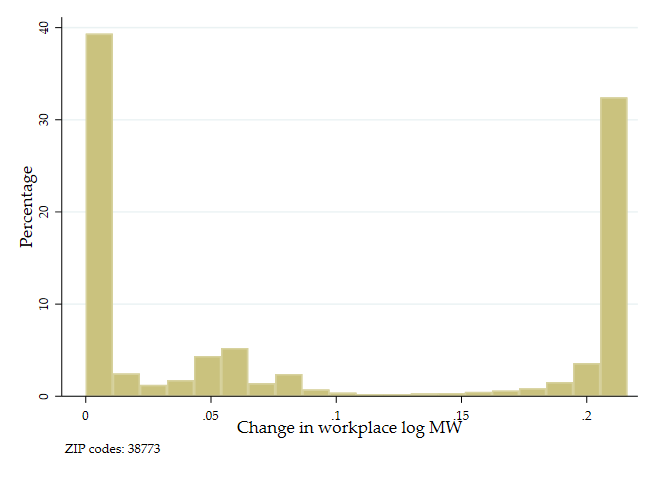
\includegraphics[width = 0.99\textwidth]{counterfactuals/output/d_exp_ln_mw_17.png}
			\caption*{Workplace MW}
		\end{subfigure}
	\end{figure}
\end{frame}

\begin{frame}
	\frametitle{Predicted increases in rents and wages}
	\begin{figure}
		\begin{subfigure}{0.51\textwidth}
			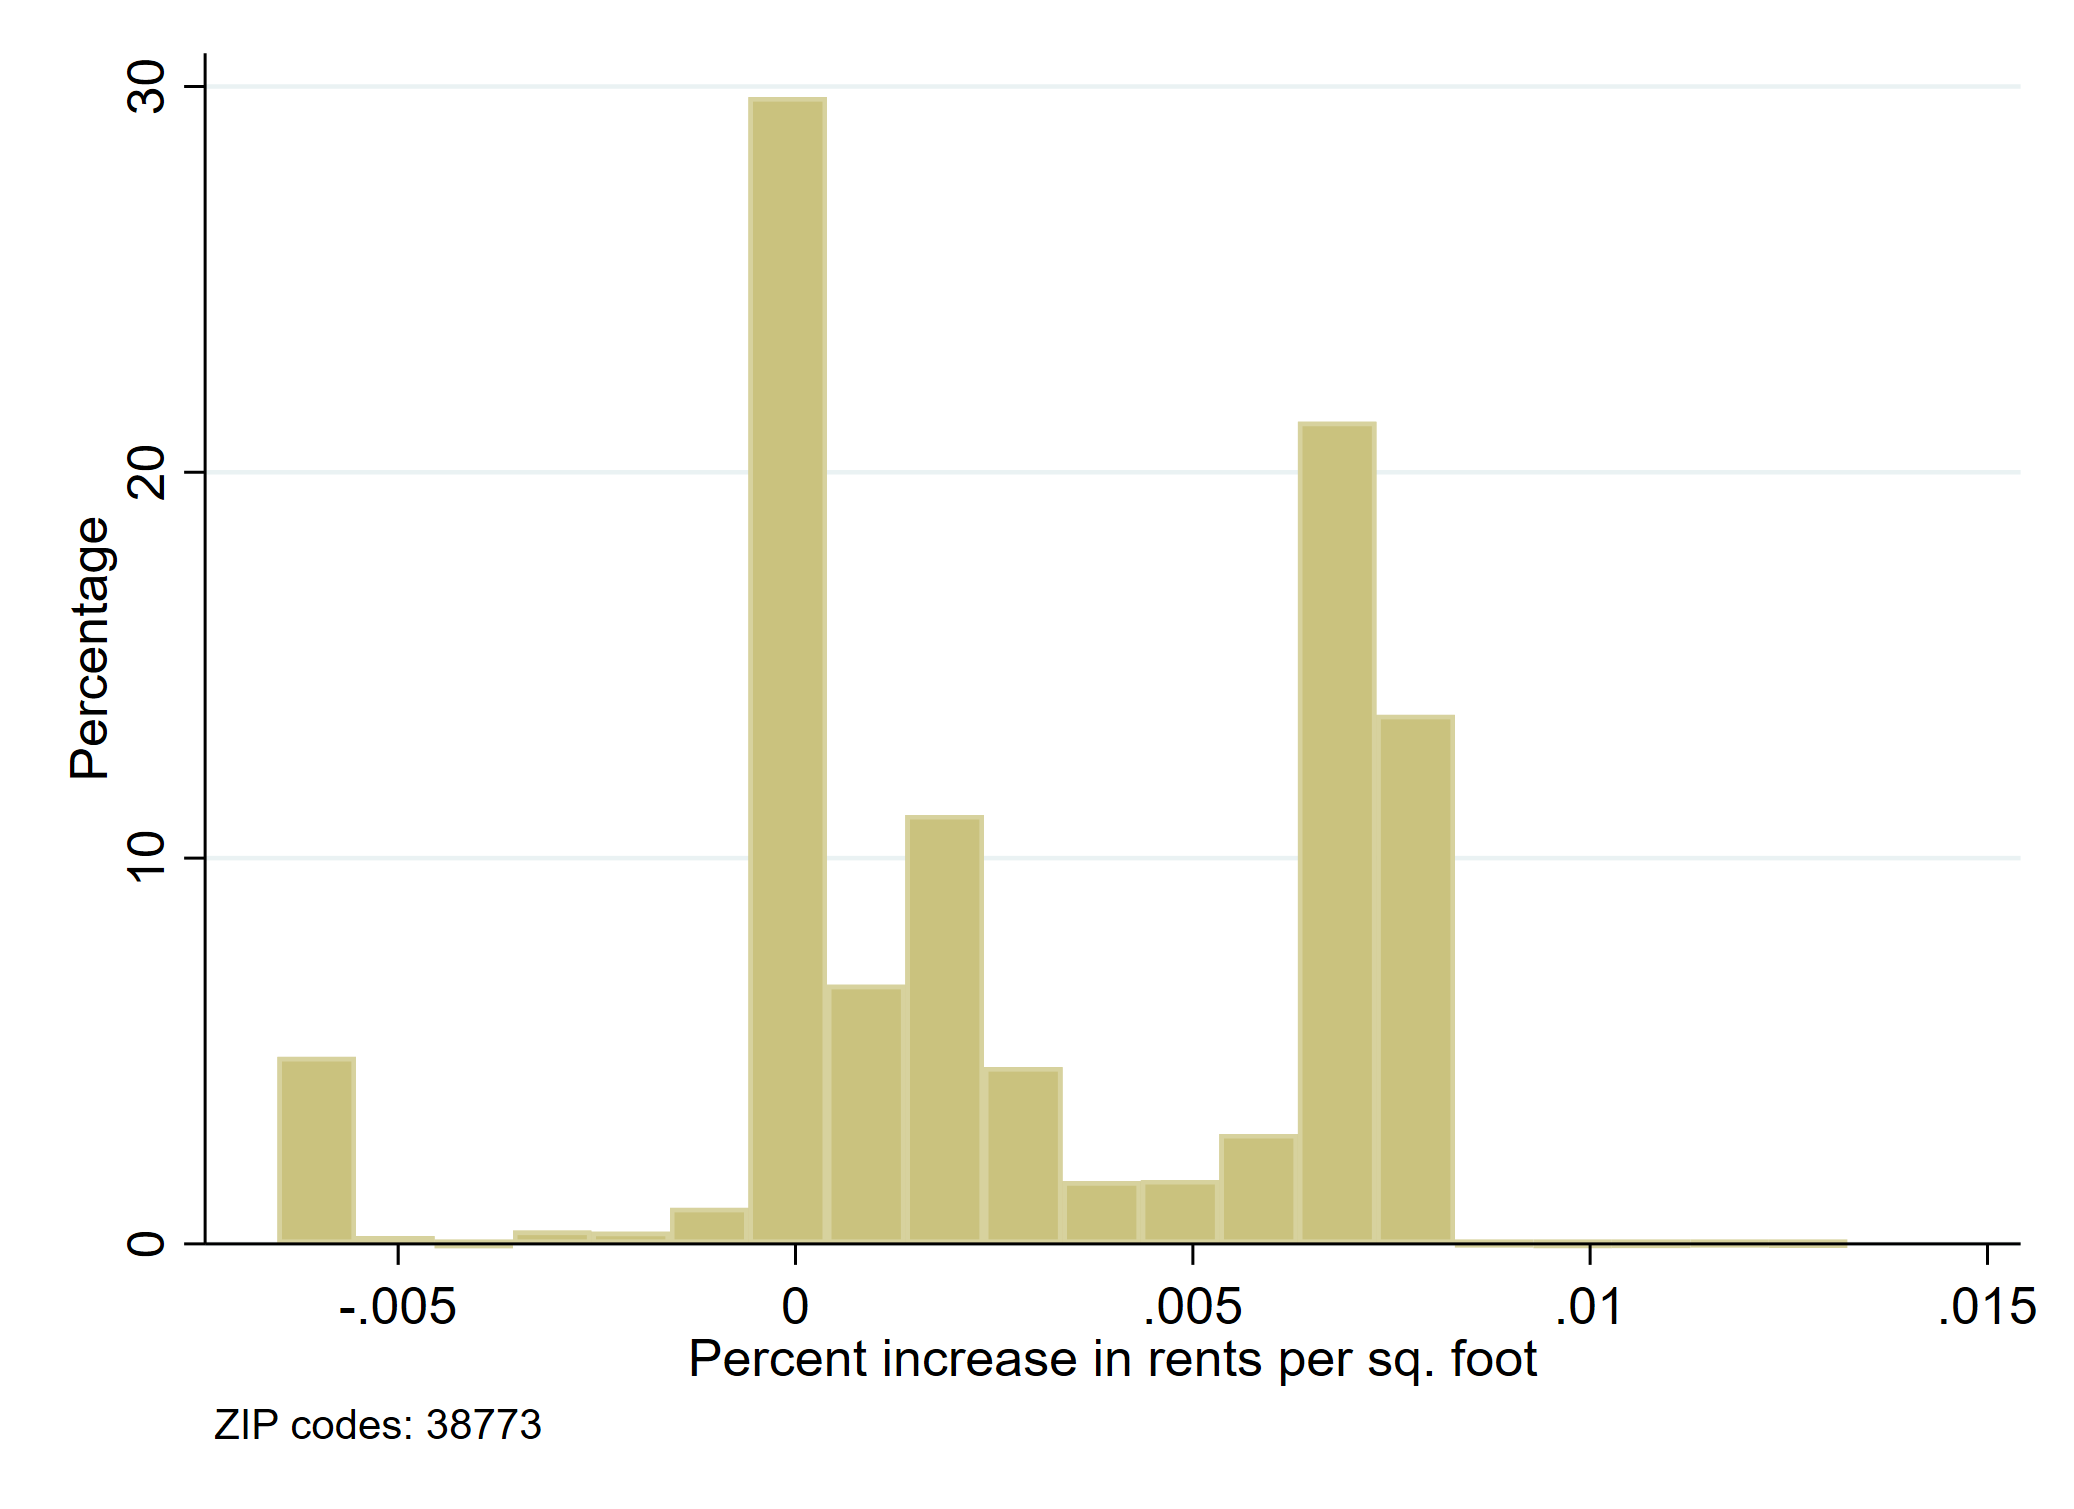
\includegraphics[width = 0.99\textwidth]{counterfactuals/output/perc_incr_rent.png}
			\caption*{Predicted changes in rents per sqft}
		\end{subfigure}%
		\begin{subfigure}{0.51\textwidth}
                         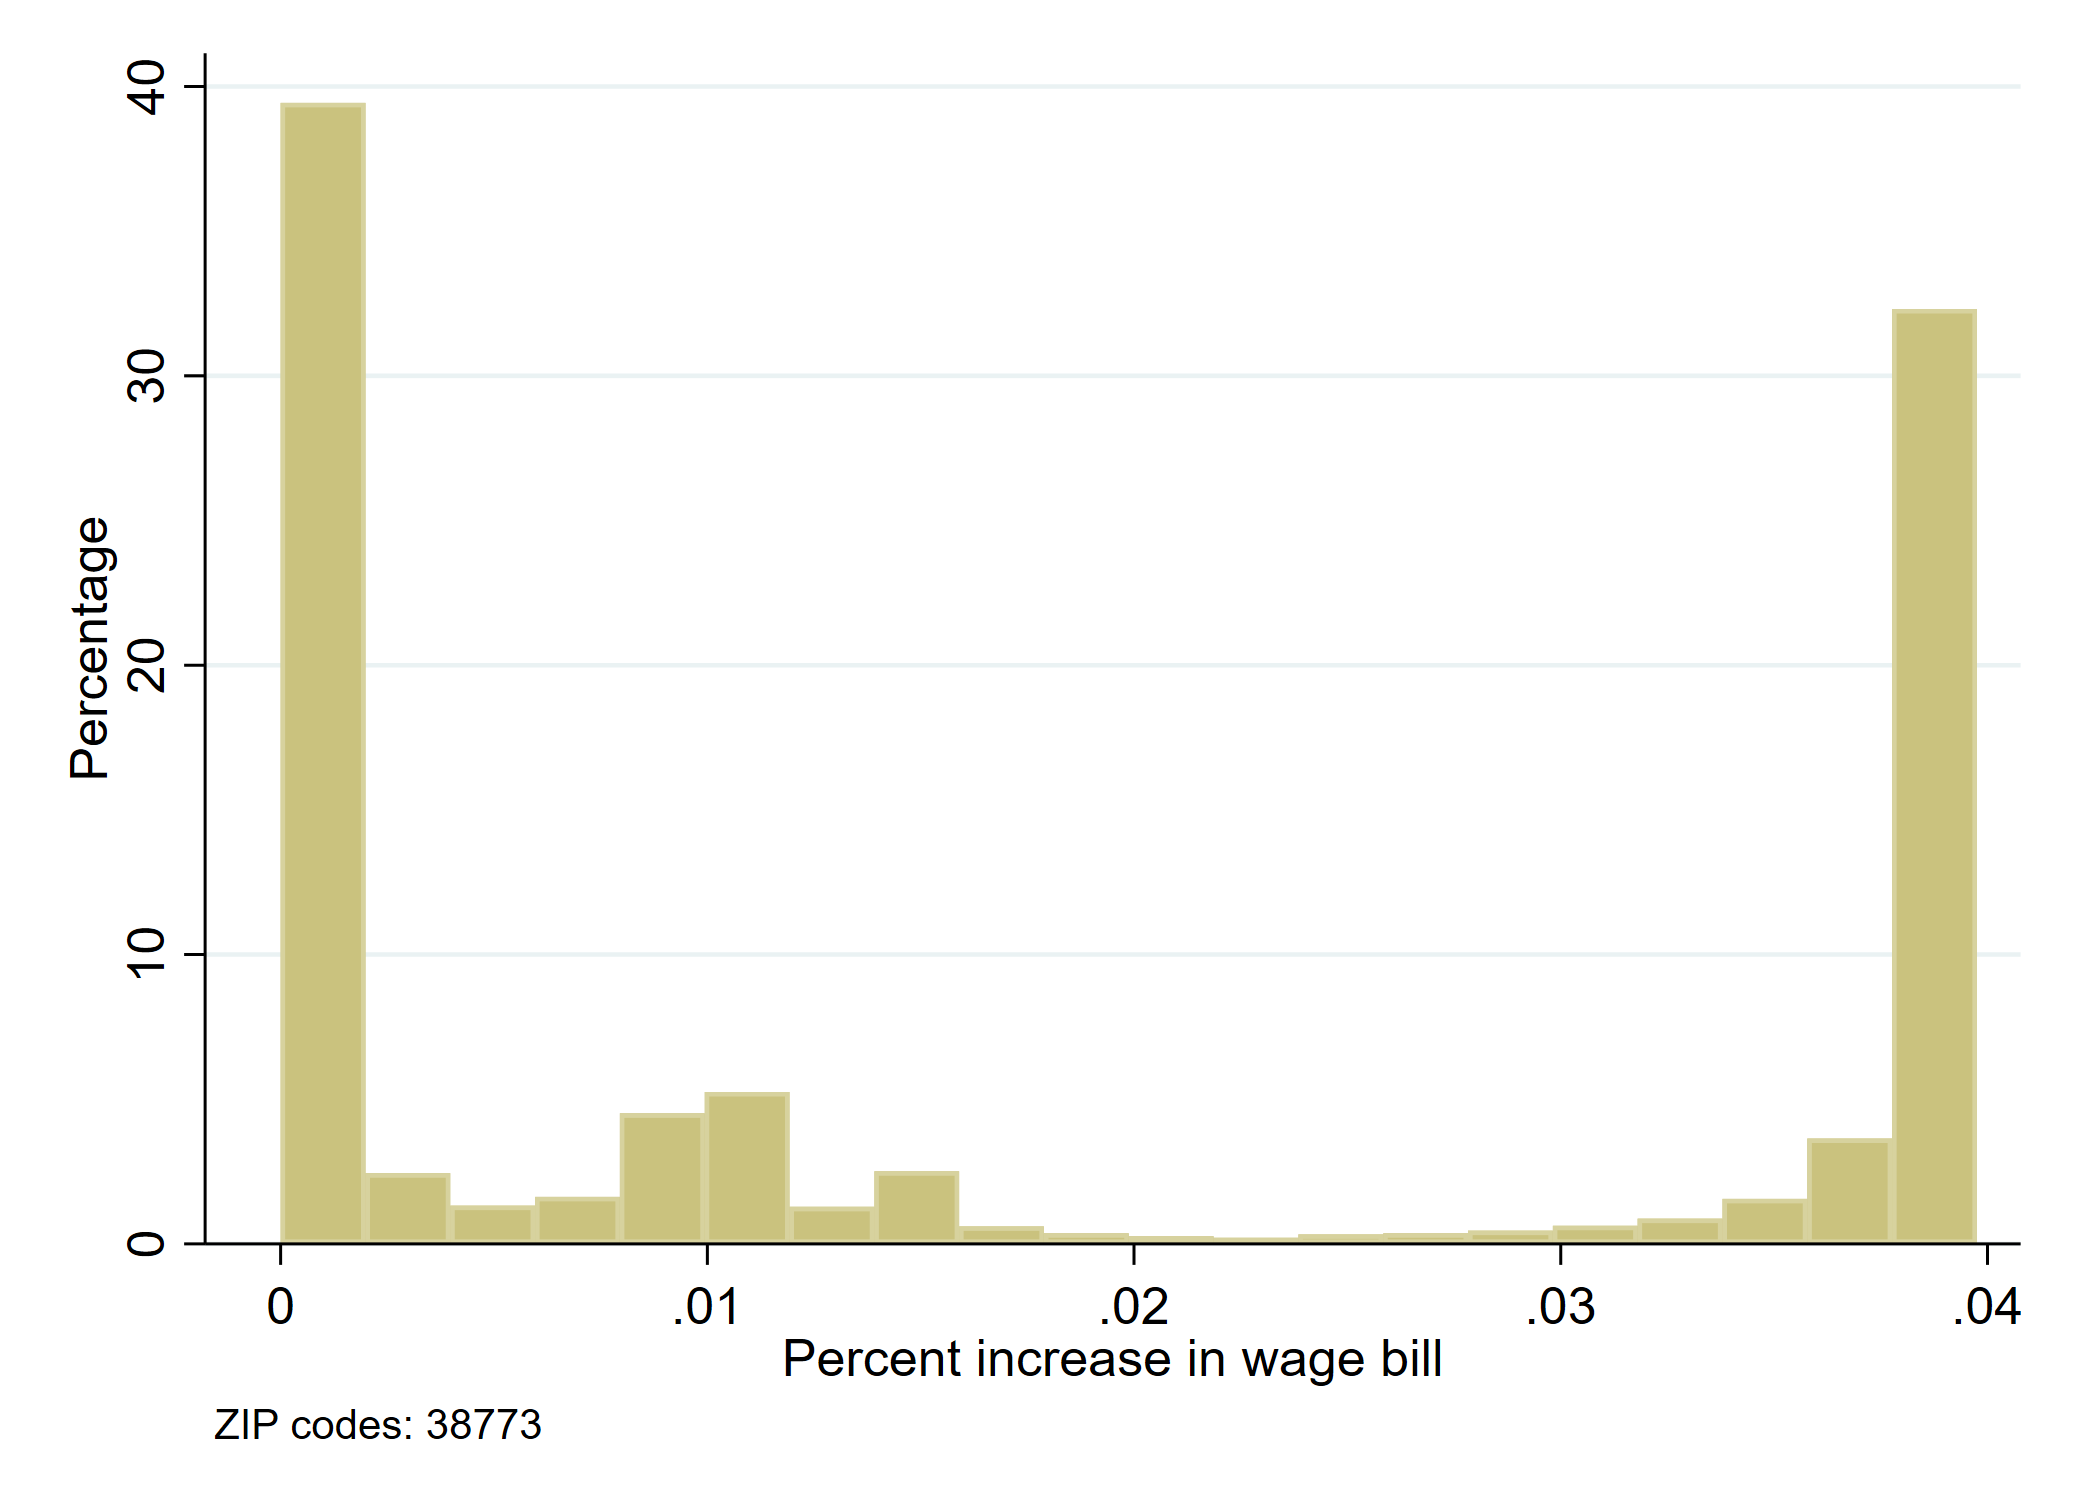
\includegraphics[width = 0.99\textwidth]{counterfactuals/output/perc_incr_wagebill.png}
			\caption*{Predicted changes in wage bill}
		\end{subfigure}
	\end{figure}	
\end{frame}

\begin{frame}
	\frametitle{Predicted gradient of rent changes in the Chicago metro area}
	\begin{figure}
		\centering
		\begin{subfigure}{0.33\textwidth}
			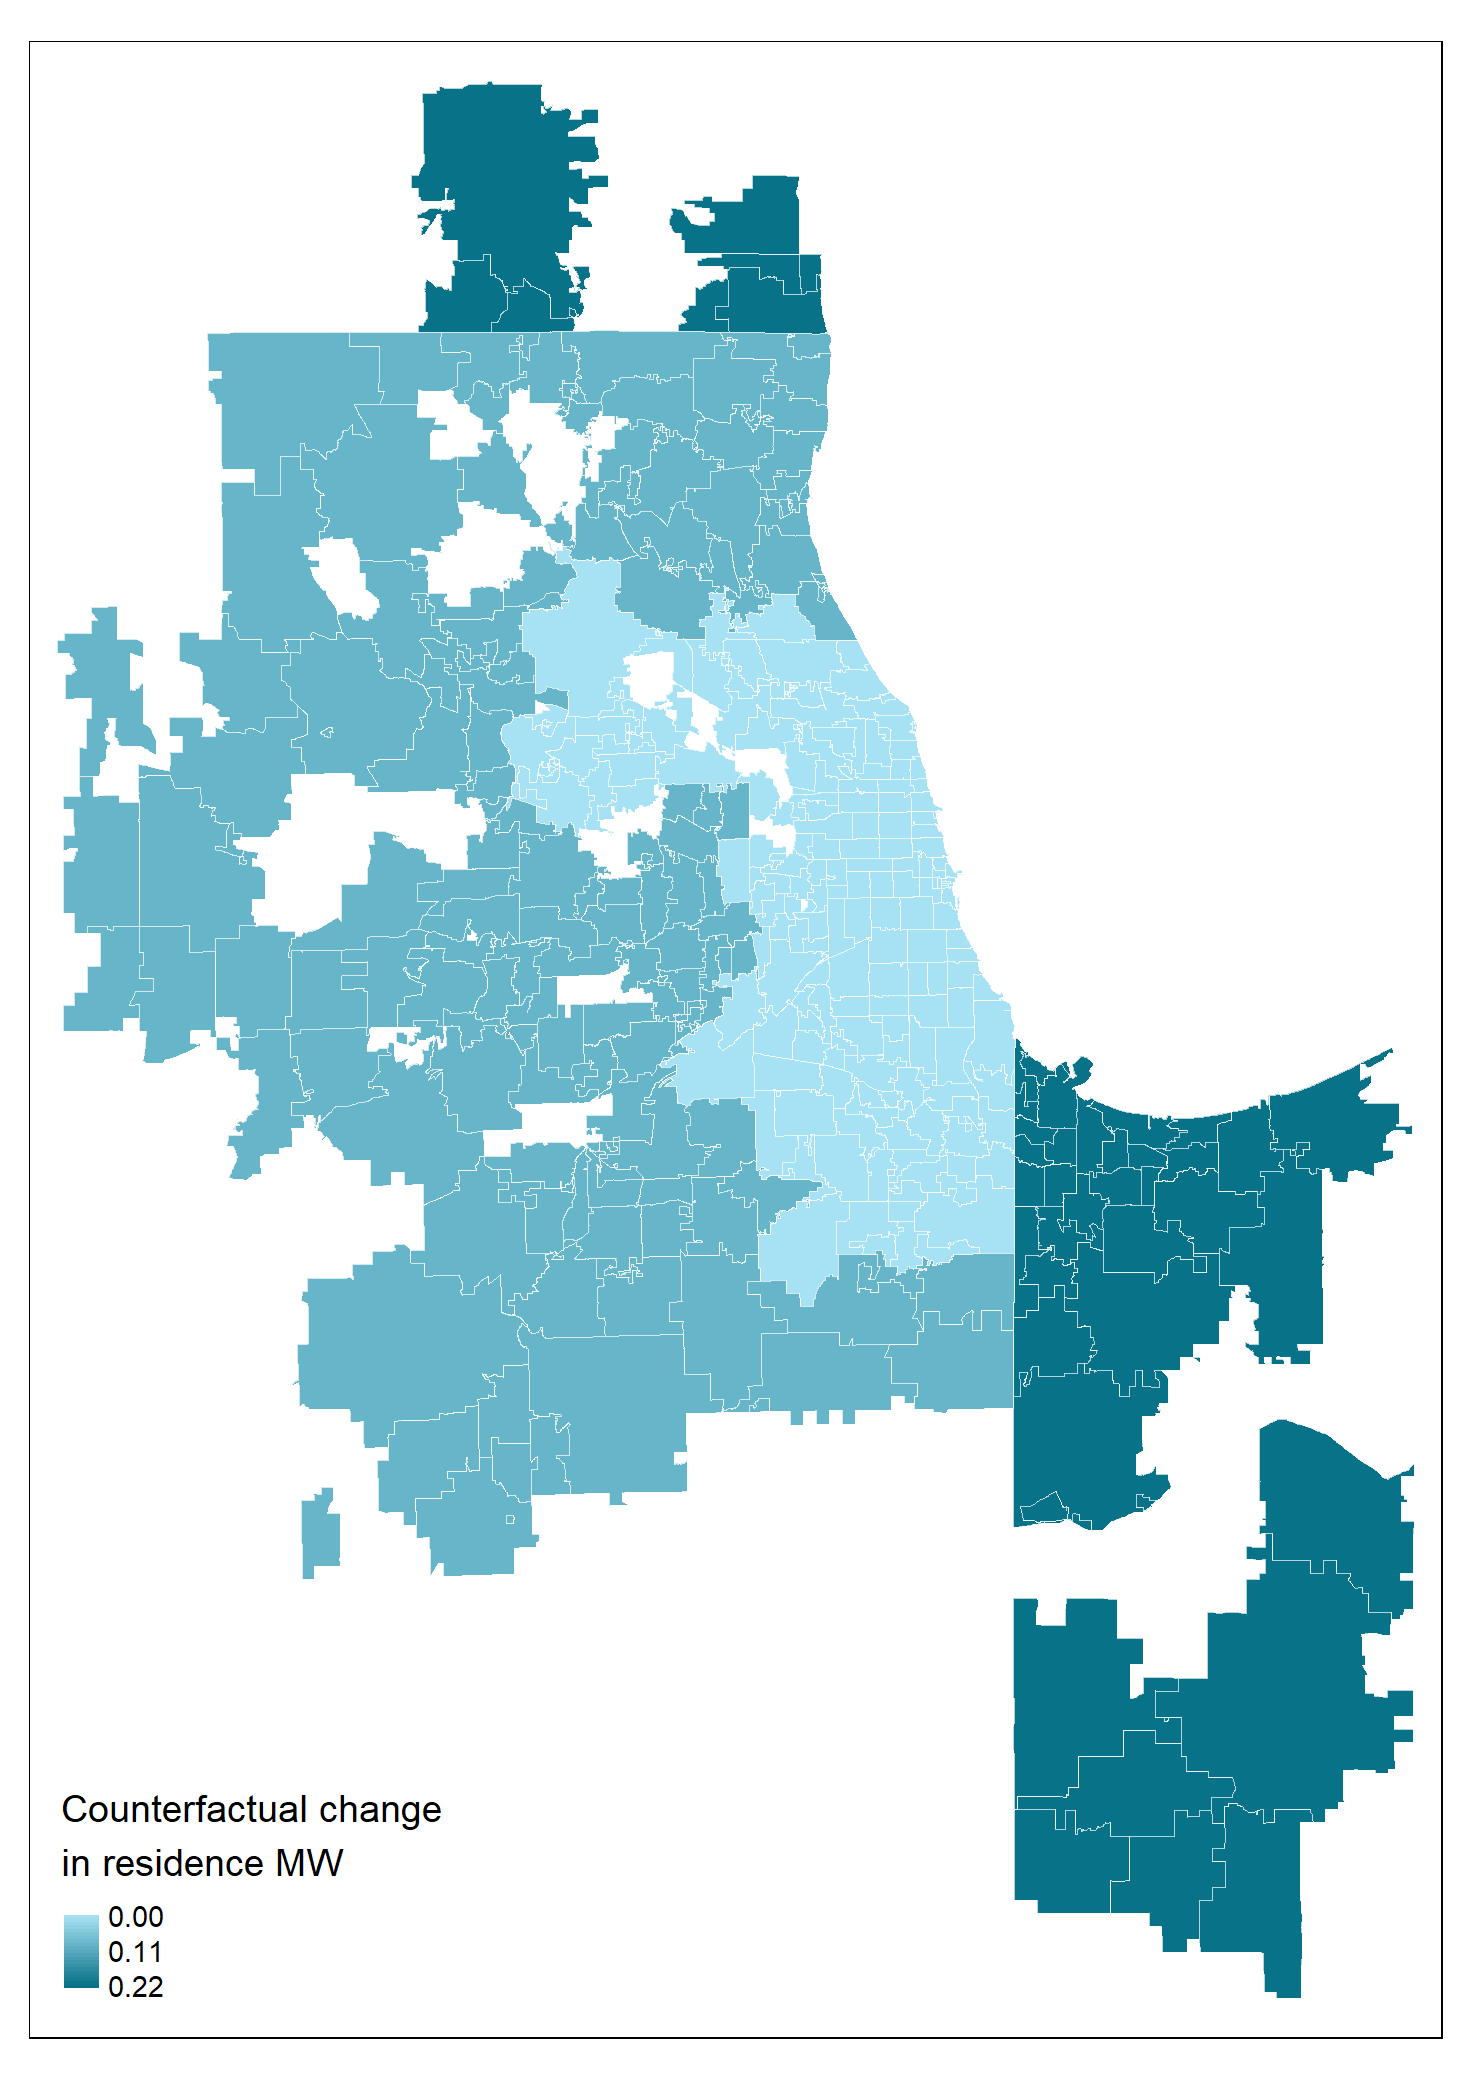
\includegraphics[width = 0.99\textwidth]{counterfactuals/output/chicago_d_ln_mw.png}
			\caption*{Counterfactual change in residence MW}
		\end{subfigure}%
		\begin{subfigure}{0.33\textwidth}
                         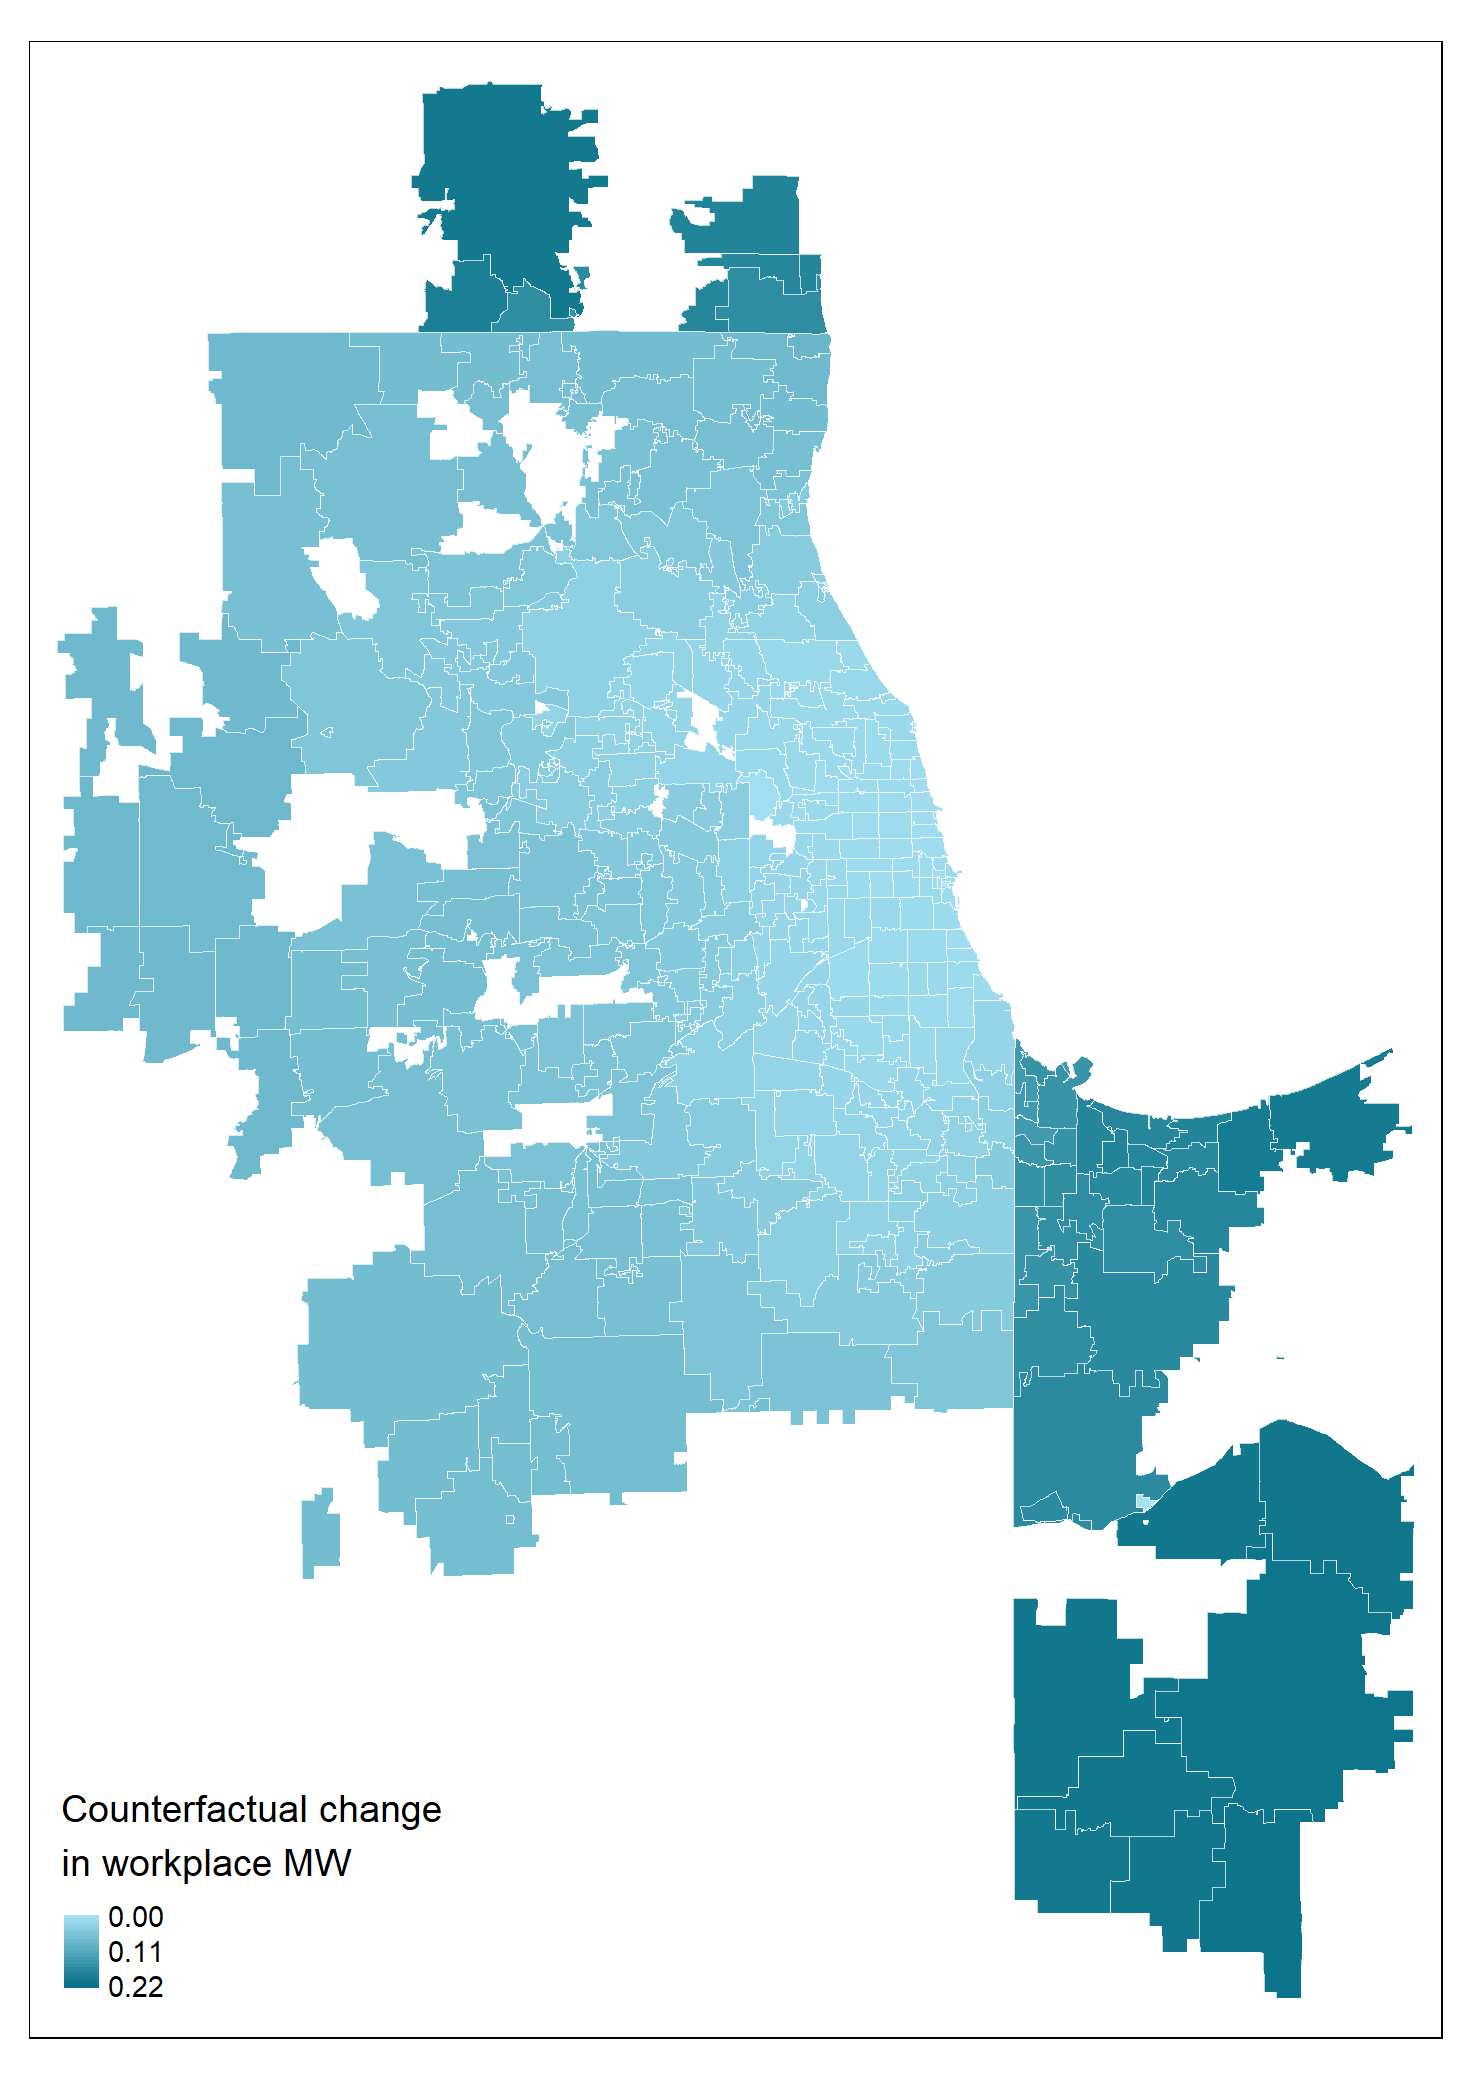
\includegraphics[width = 0.99\textwidth]{counterfactuals/output/chicago_d_exp_ln_mw.png}
			\caption*{Counterfactual change in workplace MW}
		\end{subfigure}
		\begin{subfigure}{0.33\textwidth}
                         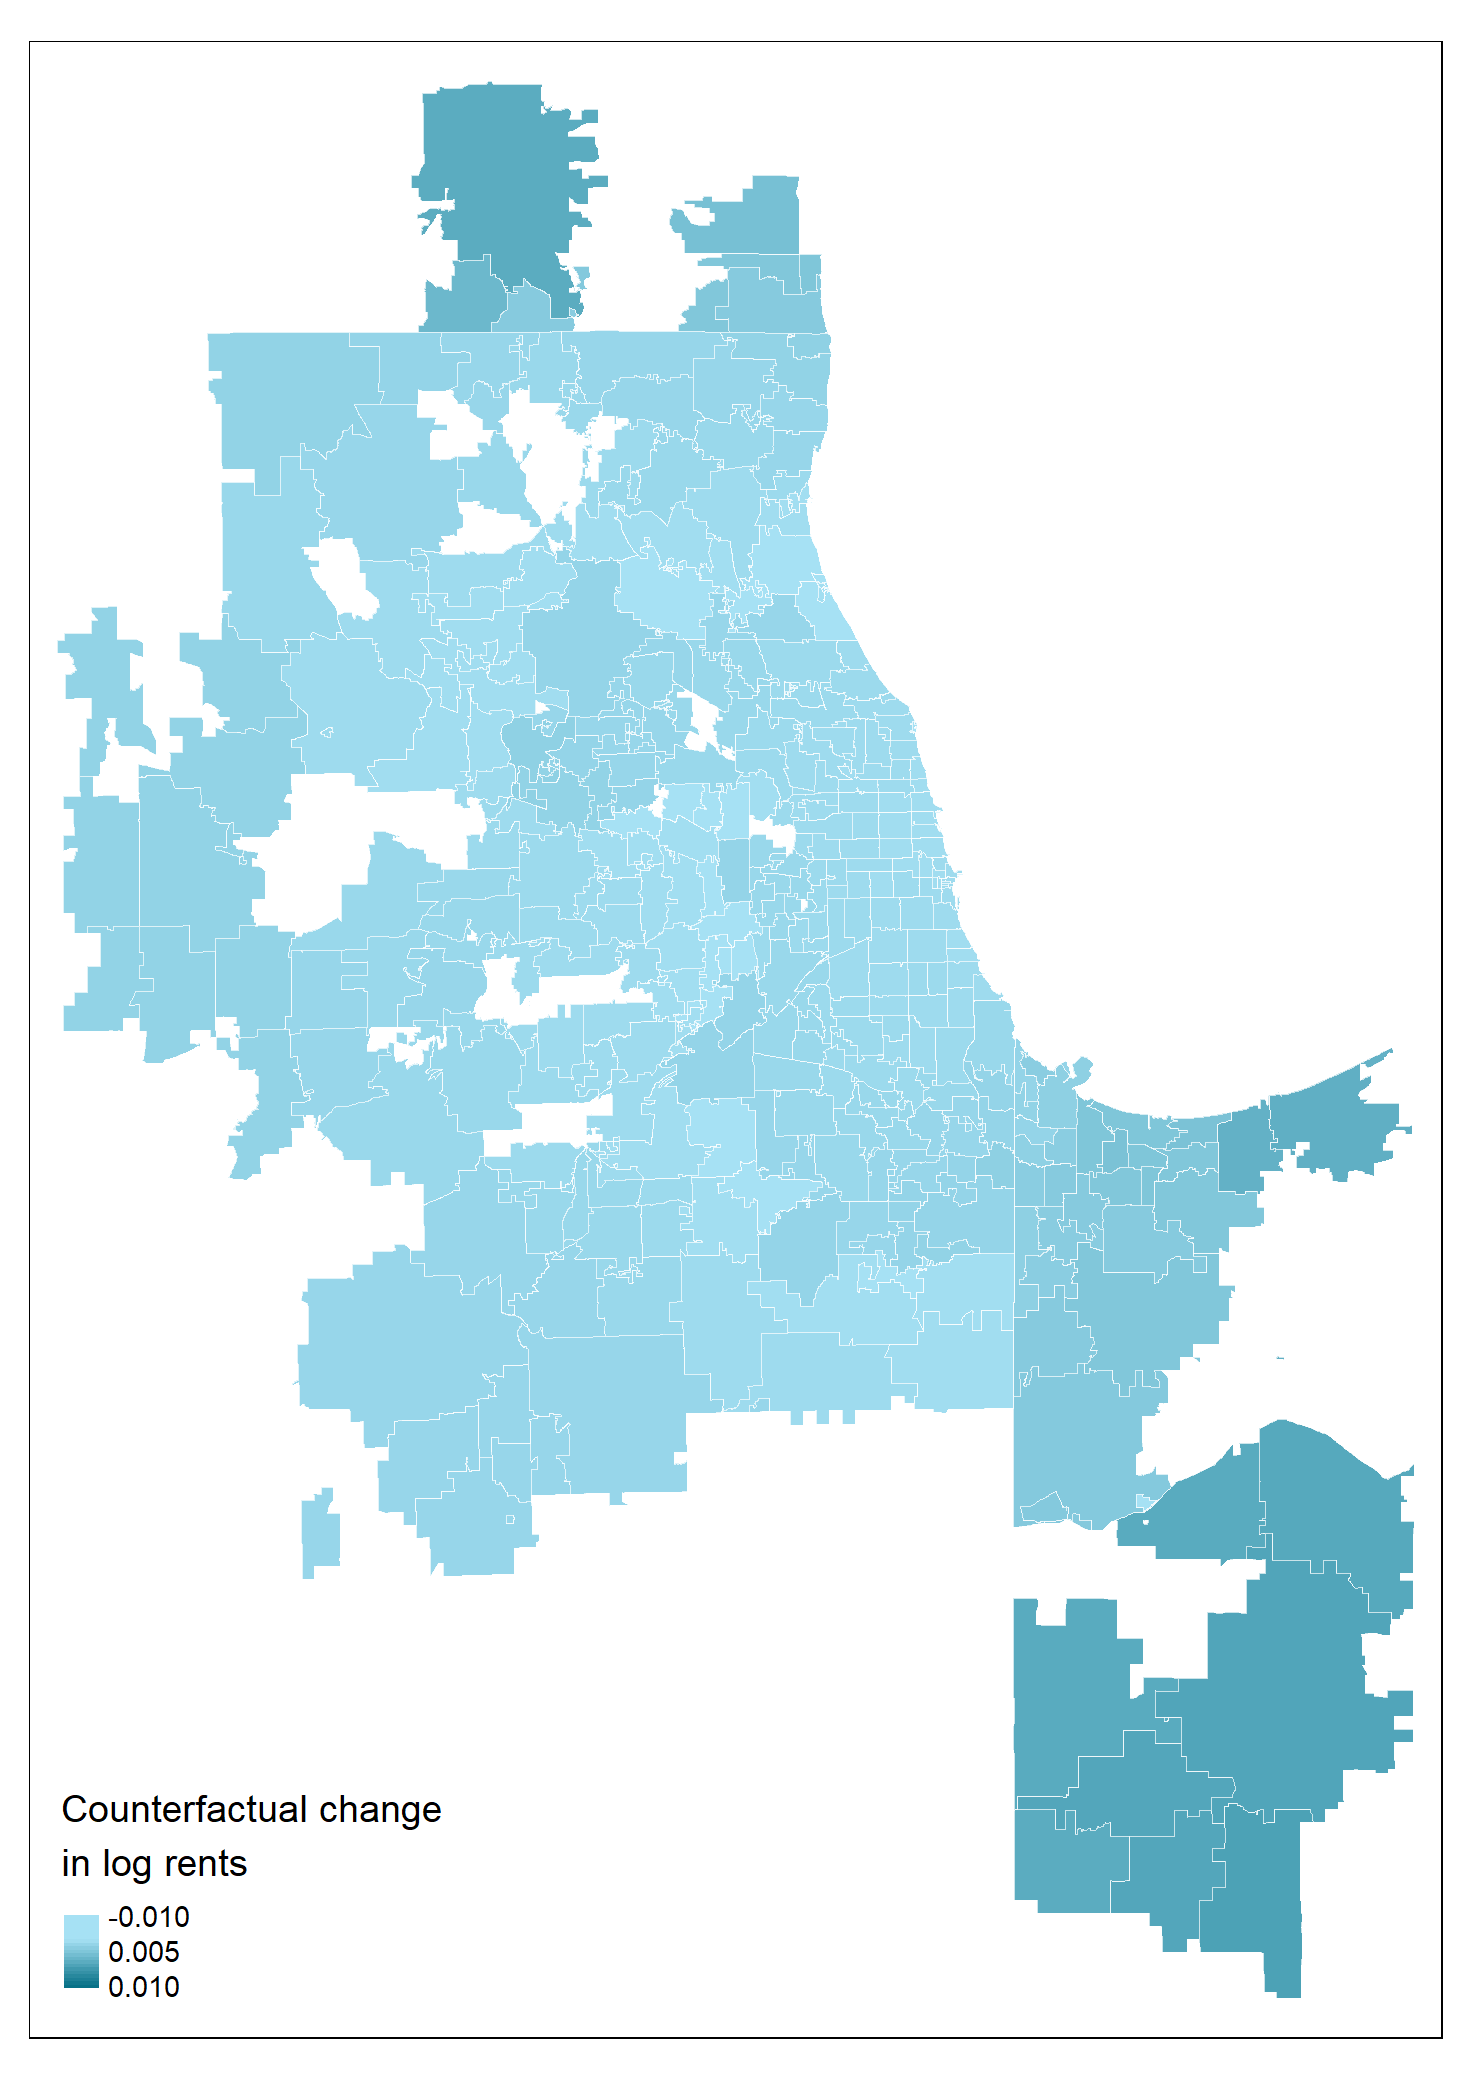
\includegraphics[width = 0.99\textwidth]{counterfactuals/output/chicago_d_ln_rents.png}
			\caption*{Counterfactual change in log rents}
		\end{subfigure}
	\end{figure}	
\end{frame}

\begin{frame}
	\frametitle{The incidence of MW changes on average}
	
	\vspace{3mm}
    \begin{table}[]

    \label{tab:counterfactuals}
    \centering
    \scalebox{0.83}{
    \begin{tabular}{@{}lcccccc@{}}
        \toprule
                            &   & \multicolumn{2}{c}{Change in log MW}
                                    & \multicolumn{1}{c}{\multirow{2}{*}{\makecell{Ratio perc.\\increases}}} 
                                             & \multicolumn{2}{c}{Landlord share for $\alpha$}   \\ \cmidrule(lr){3-4} \cmidrule(l){6-7}
                            & N & Res.\ & Wrk.\
                                    & \multicolumn{1}{c}{}        
                                             & 0.25  & 0.45     \\ \midrule
        Effect in ZIP codes...                           &      &         &       &       &                &                 \\
        $\quad$with previous res. MW $\leq\$9\quad$    & 8,753 &  0.216   &  0.183  &  0.180  & 0.045 &  0.081   \\
        $\quad$with previous res. MW $>\$9\quad$       & 5,555 &  0   &  0.004  &  0.357  & 0.089  & 0.161   \\ \bottomrule
    \end{tabular}
    }
    \begin{minipage}{.95\textwidth} \footnotesize
        \vspace{2mm}
        Notes: The table shows computations of the pass-through share for the following
        parameters: $\beta = 0.064$, $\gamma = -0.030$, $\varepsilon = 0.180$, and $\alpha\in\{0.25, 0.45\}$.
    \end{minipage}
\end{table}


	\pause
	\vspace{3mm}

	More generally, one can think of the effect for different values of 
	$$
		\Delta \MW_i^{wrk} - \Delta \MW_i^{res}
	$$
\end{frame}

\begin{frame}
	\frametitle{The incidence of MW changes according to intensity of treatment}
	
	\begin{figure}
		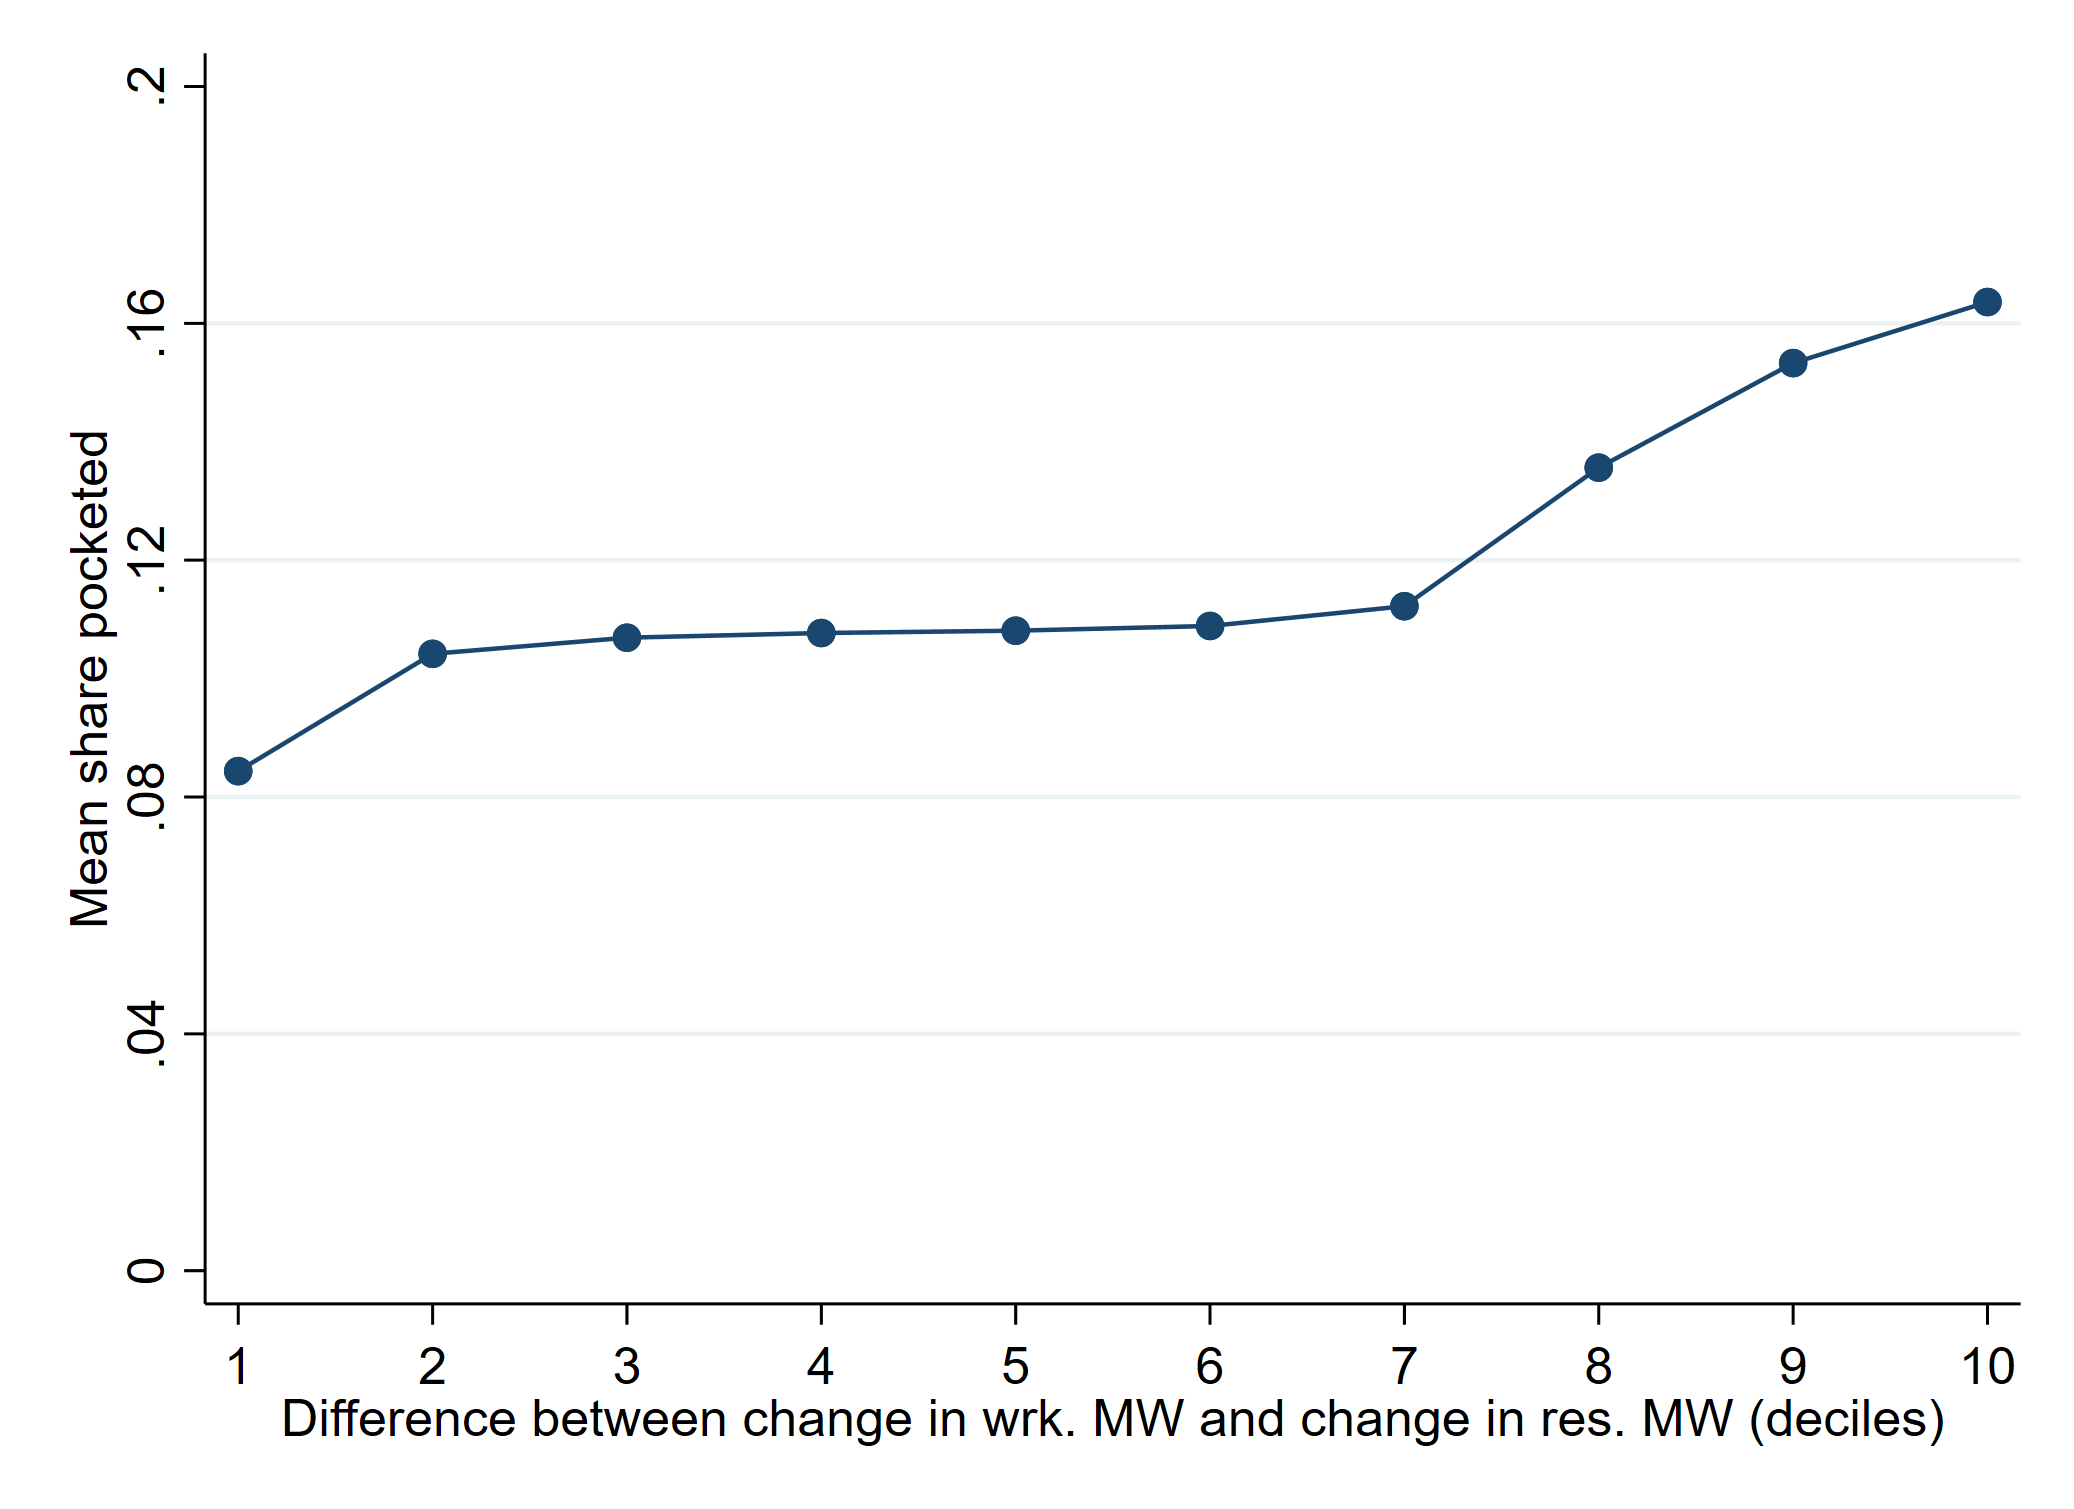
\includegraphics[width = 0.65\textwidth]{counterfactuals/output/deciles_diff.png}
		\begin{minipage}{.95\textwidth} \footnotesize
			\vspace{2mm}
			Notes: The figure shows computations of the pass-through share for the following
			parameters: $\beta = 0.064$, $\gamma = -0.030$, $\varepsilon = 0.180$, and $\alpha=0.35$.
		\end{minipage}
	\end{figure}
\end{frame}

\section{Concluding remarks}

\begin{frame}
	\frametitle{Conclusion}
	
	\begin{itemize}
	    \item When studying effects of place-based policies on the housing market it is crucial
	     to account for the fact that agents live and work in different locations.
		 \vspace{1mm}
	     \item We estimate an elasticity of workplace MW to rents of about $0.065$, and of residence MW of $-0.03$.
		 \vspace{1mm}
	     \item Our estimates imply that landlords pocket between 5 and 15 cents cents on the dollar of the extra 
	     income that MW policies put on the table.
		 \vspace{1mm}
	     \item Landlords in areas right outside of where the MW policies are implemented are those that are set to extract the most rents. 
	     \item Even with a two-parameter model, we are able to describe and predict rich patterns in the rental markets.
	\end{itemize}
	
\end{frame}

\begin{frame}[c]
    \begin{center}
    	\Large Thank You!
    \end{center}
\end{frame}

%%%%%%%%%%%%%%%%%%%%%%%%%%%%%%%%%%%%%%%%%%%%%%%%%%%%%%%%%%%%%%%%%%%%%%%%%%%%%%%%%%%%%%%%%%
%                                       APPENDIX                                        %
%%%%%%%%%%%%%%%%%%%%%%%%%%%%%%%%%%%%%%%%%%%%%%%%%%%%%%%%%%%%%%%%%%%%%%%%%%%%%%%%%%%%%%%%%%

\appendix

\renewcommand\thetable{\thesection.\arabic{table}} 
\renewcommand\thefigure{\thesection.\arabic{figure}} 
\setcounter{table}{0}
\setcounter{figure}{0}

\section{Appendix}

\begin{frame}[label = nyc_example]
\frametitle{New York (MW changes in January 2019)}
    \begin{columns}
        \begin{column}{0.50\textwidth}
            \vspace{-4mm}
            \begin{figure}
                \centering
                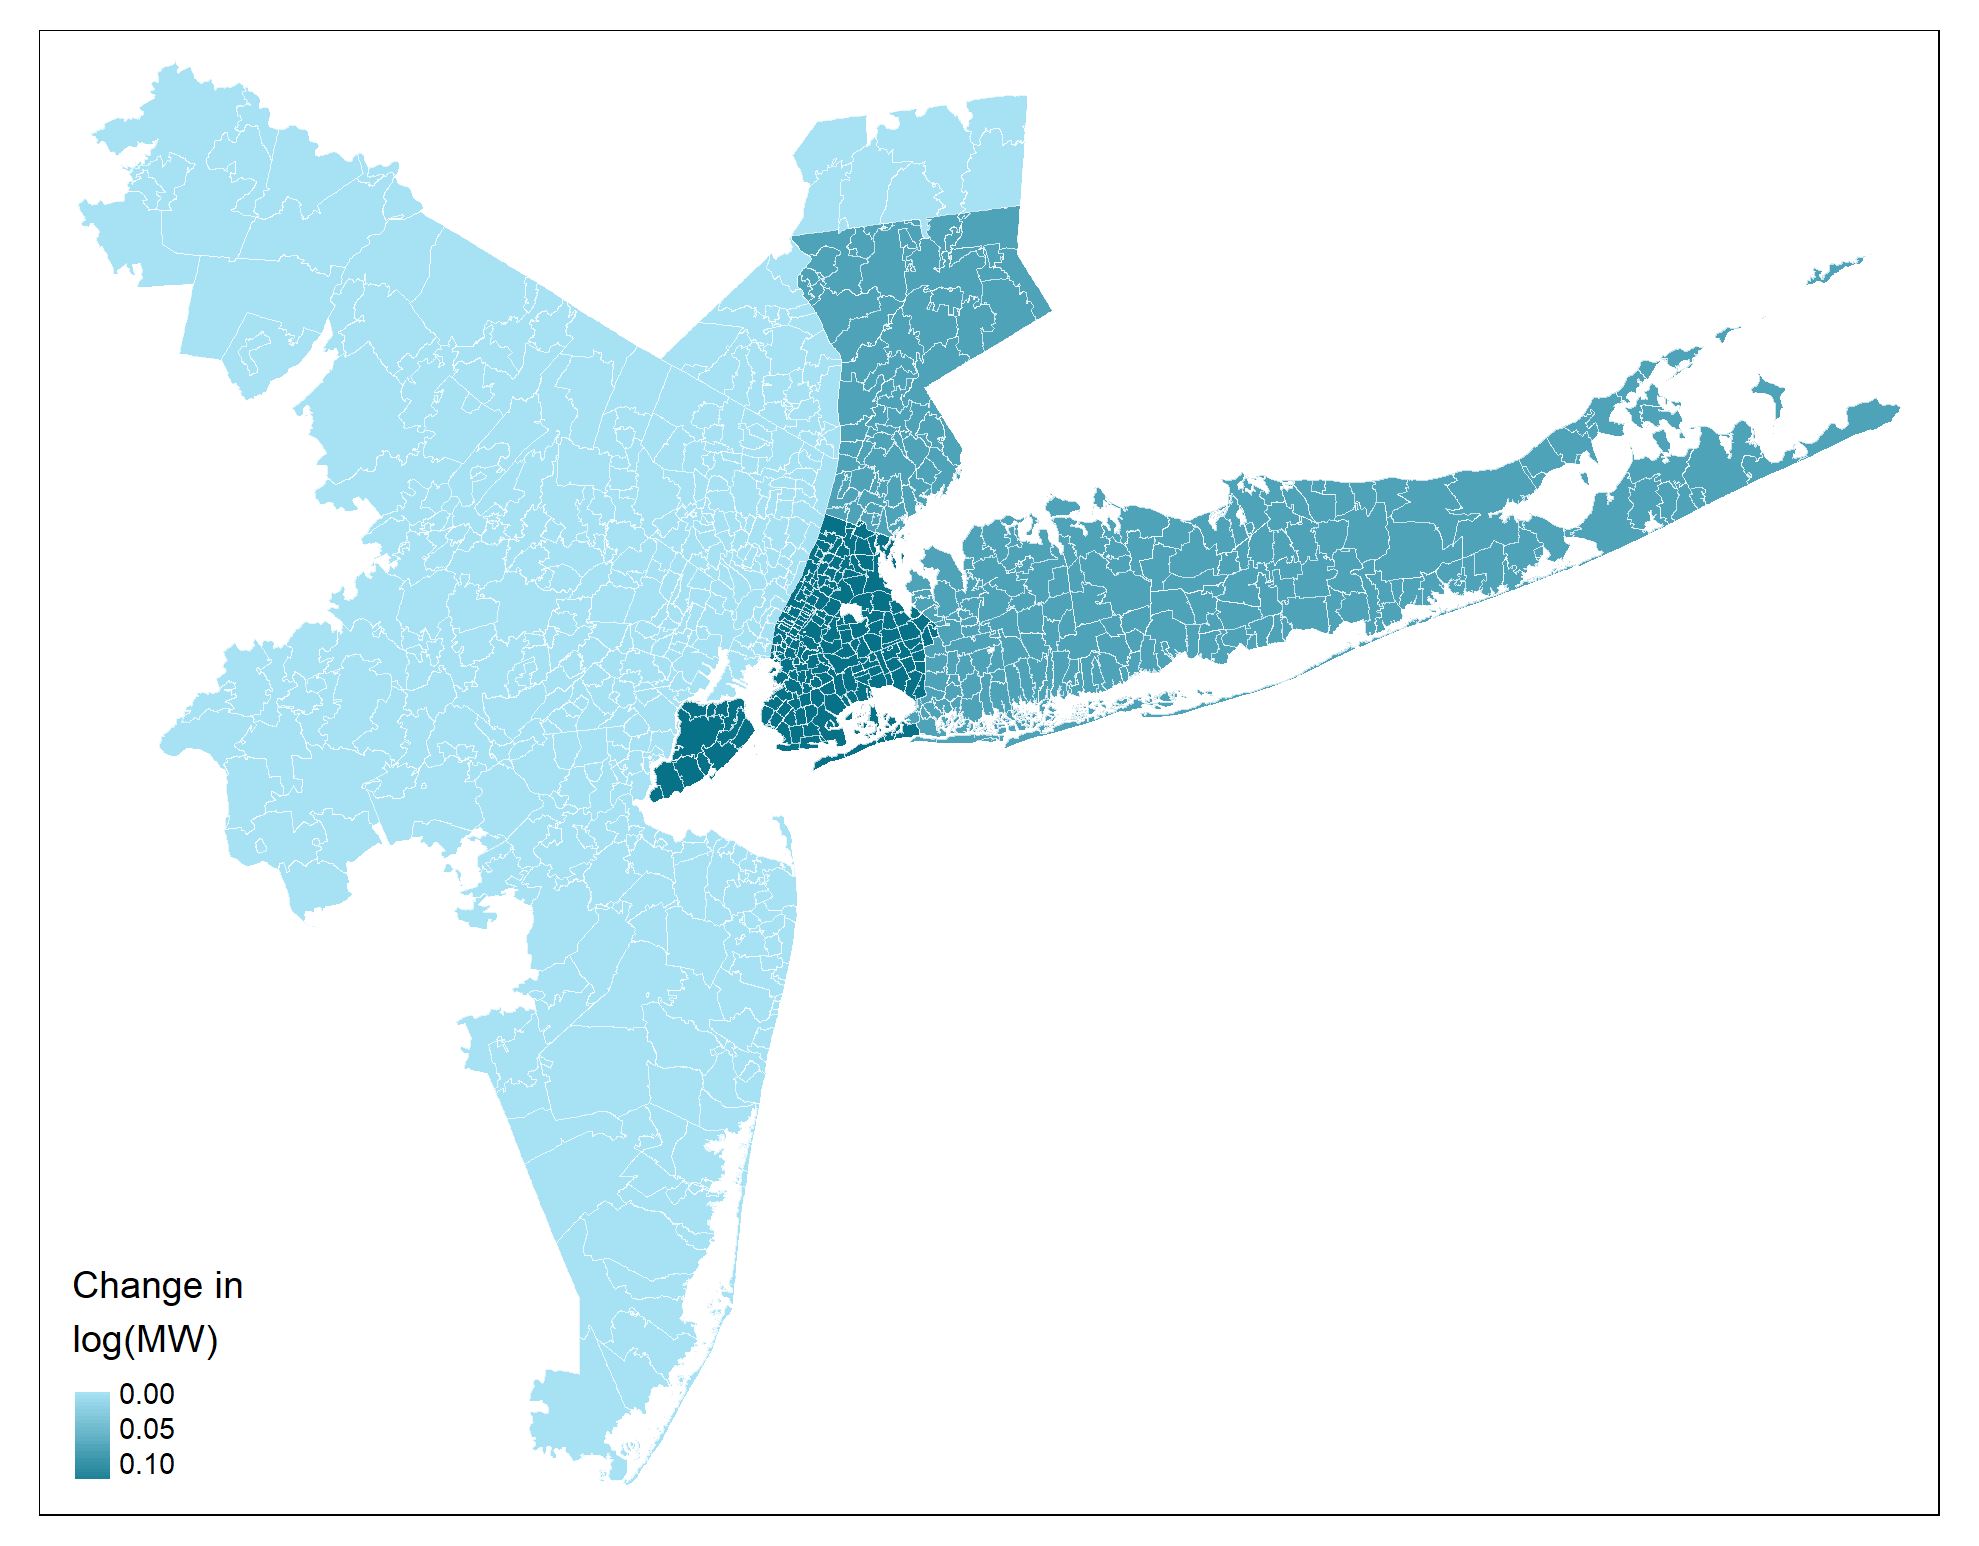
\includegraphics[scale = 0.36]{maps_events/output/nyc_2018-12_actual_mw.png}
            \end{figure}   
        \end{column}
        \begin{column}{0.50\textwidth}
            \vspace{-4mm}
            \begin{figure}
                \centering
                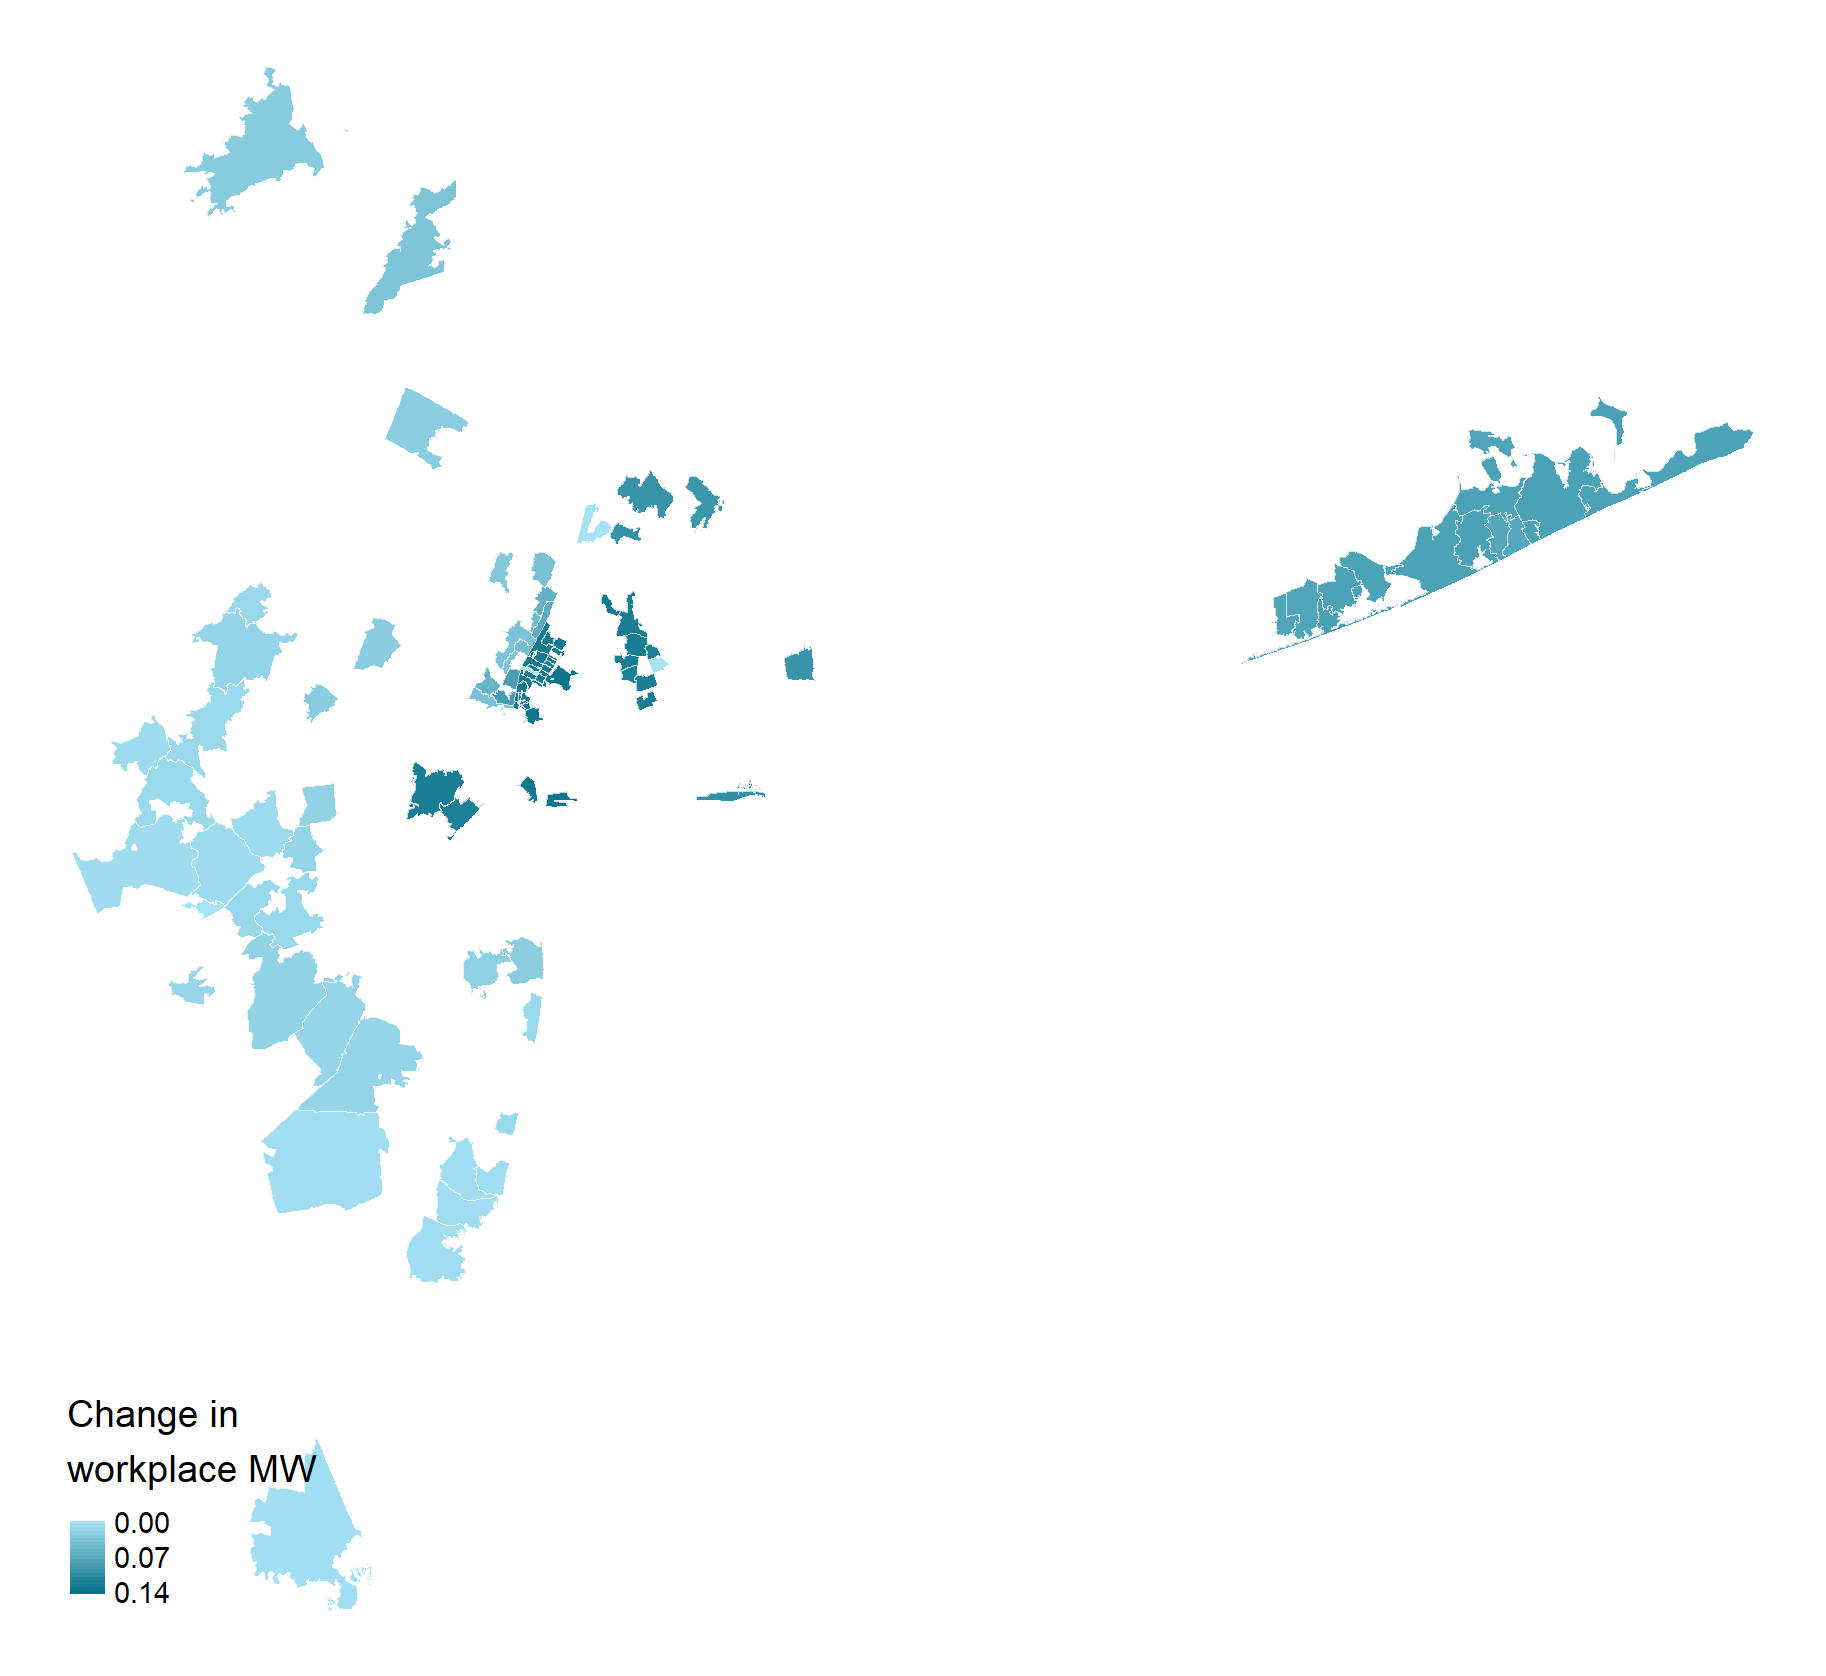
\includegraphics[scale = 0.36]{maps_events/output/nyc2018-12_exp_mw.png}
            \end{figure}   
        \end{column}
    \end{columns}
    \hyperlink{chi_example}{\beamerbutton{Go back}}
\end{frame}

\begin{frame}[label = bay_example]
\frametitle{Bay area (MW changes in January 2019)}
    \begin{columns}
        \begin{column}{0.50\textwidth}
            \vspace{-4mm}
            \begin{figure}
                \centering
                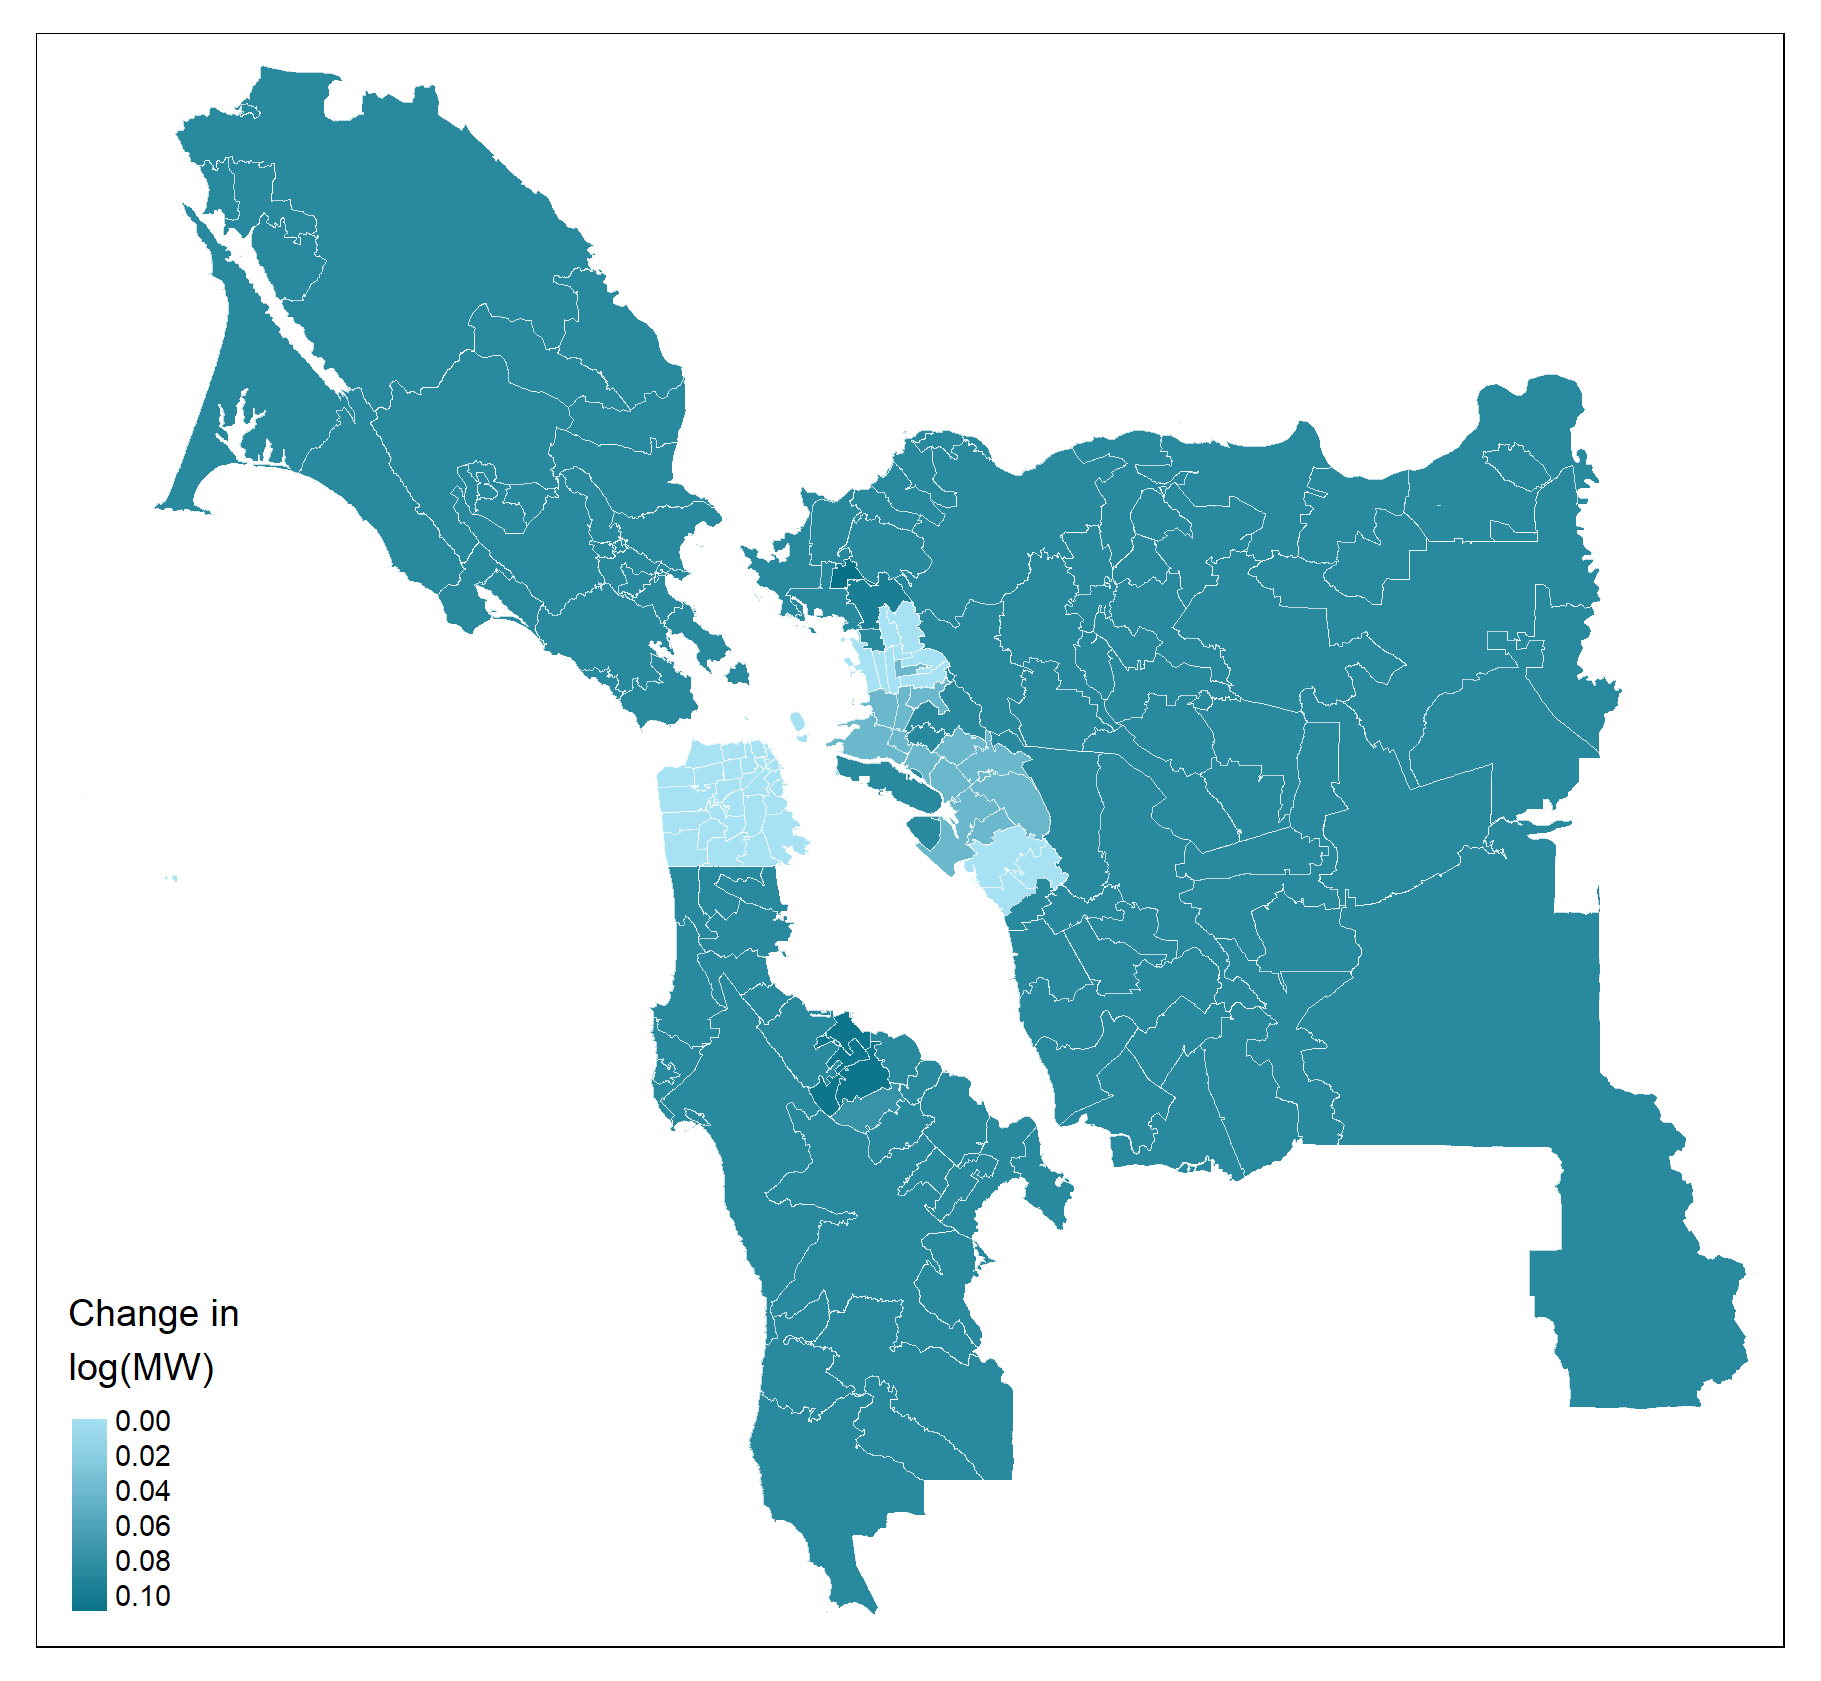
\includegraphics[scale = 0.36]{maps_events/output/bay_area_2018-12_actual_mw.png}
            \end{figure}   
        \end{column}
        \begin{column}{0.50\textwidth}
            \vspace{-4mm}
            \begin{figure}
                \centering
                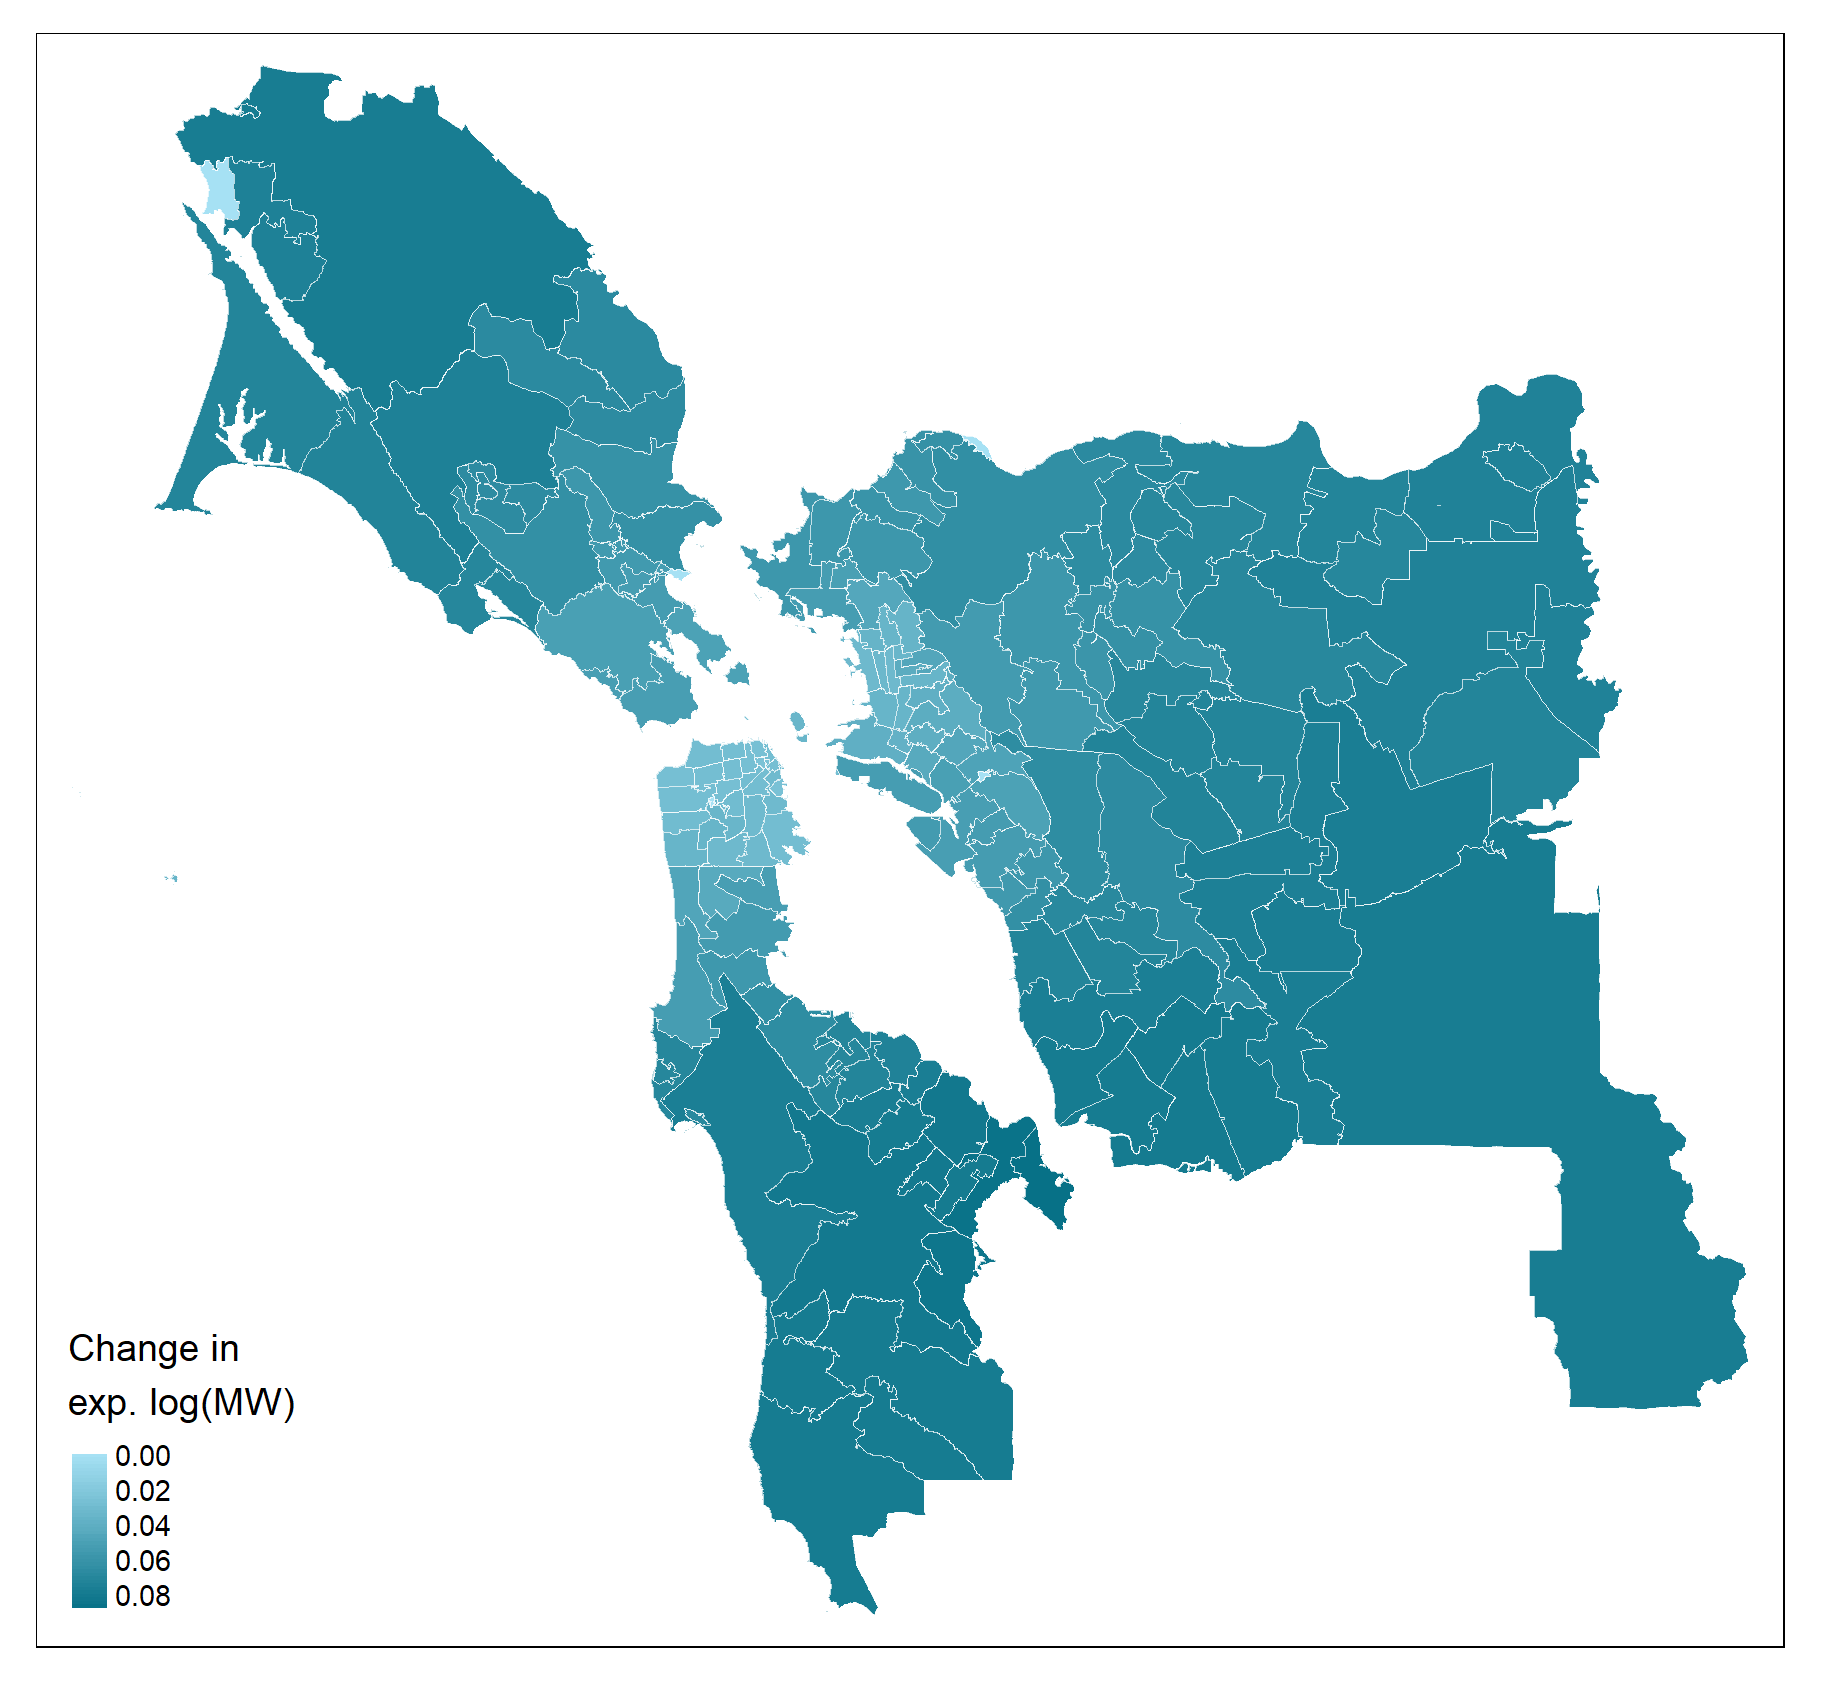
\includegraphics[scale = 0.36]{maps_events/output/bay_area2018-12_exp_mw.png}
            \end{figure}   
        \end{column}
    \end{columns}
    \hyperlink{chi_example}{\beamerbutton{Go back}}
\end{frame}

\begin{frame}[label = seattle_example]
\frametitle{Seattle (MW changes in January 2018)}
    \begin{columns}
        \begin{column}{0.50\textwidth}
            \vspace{-4mm}
            \begin{figure}
                \centering
                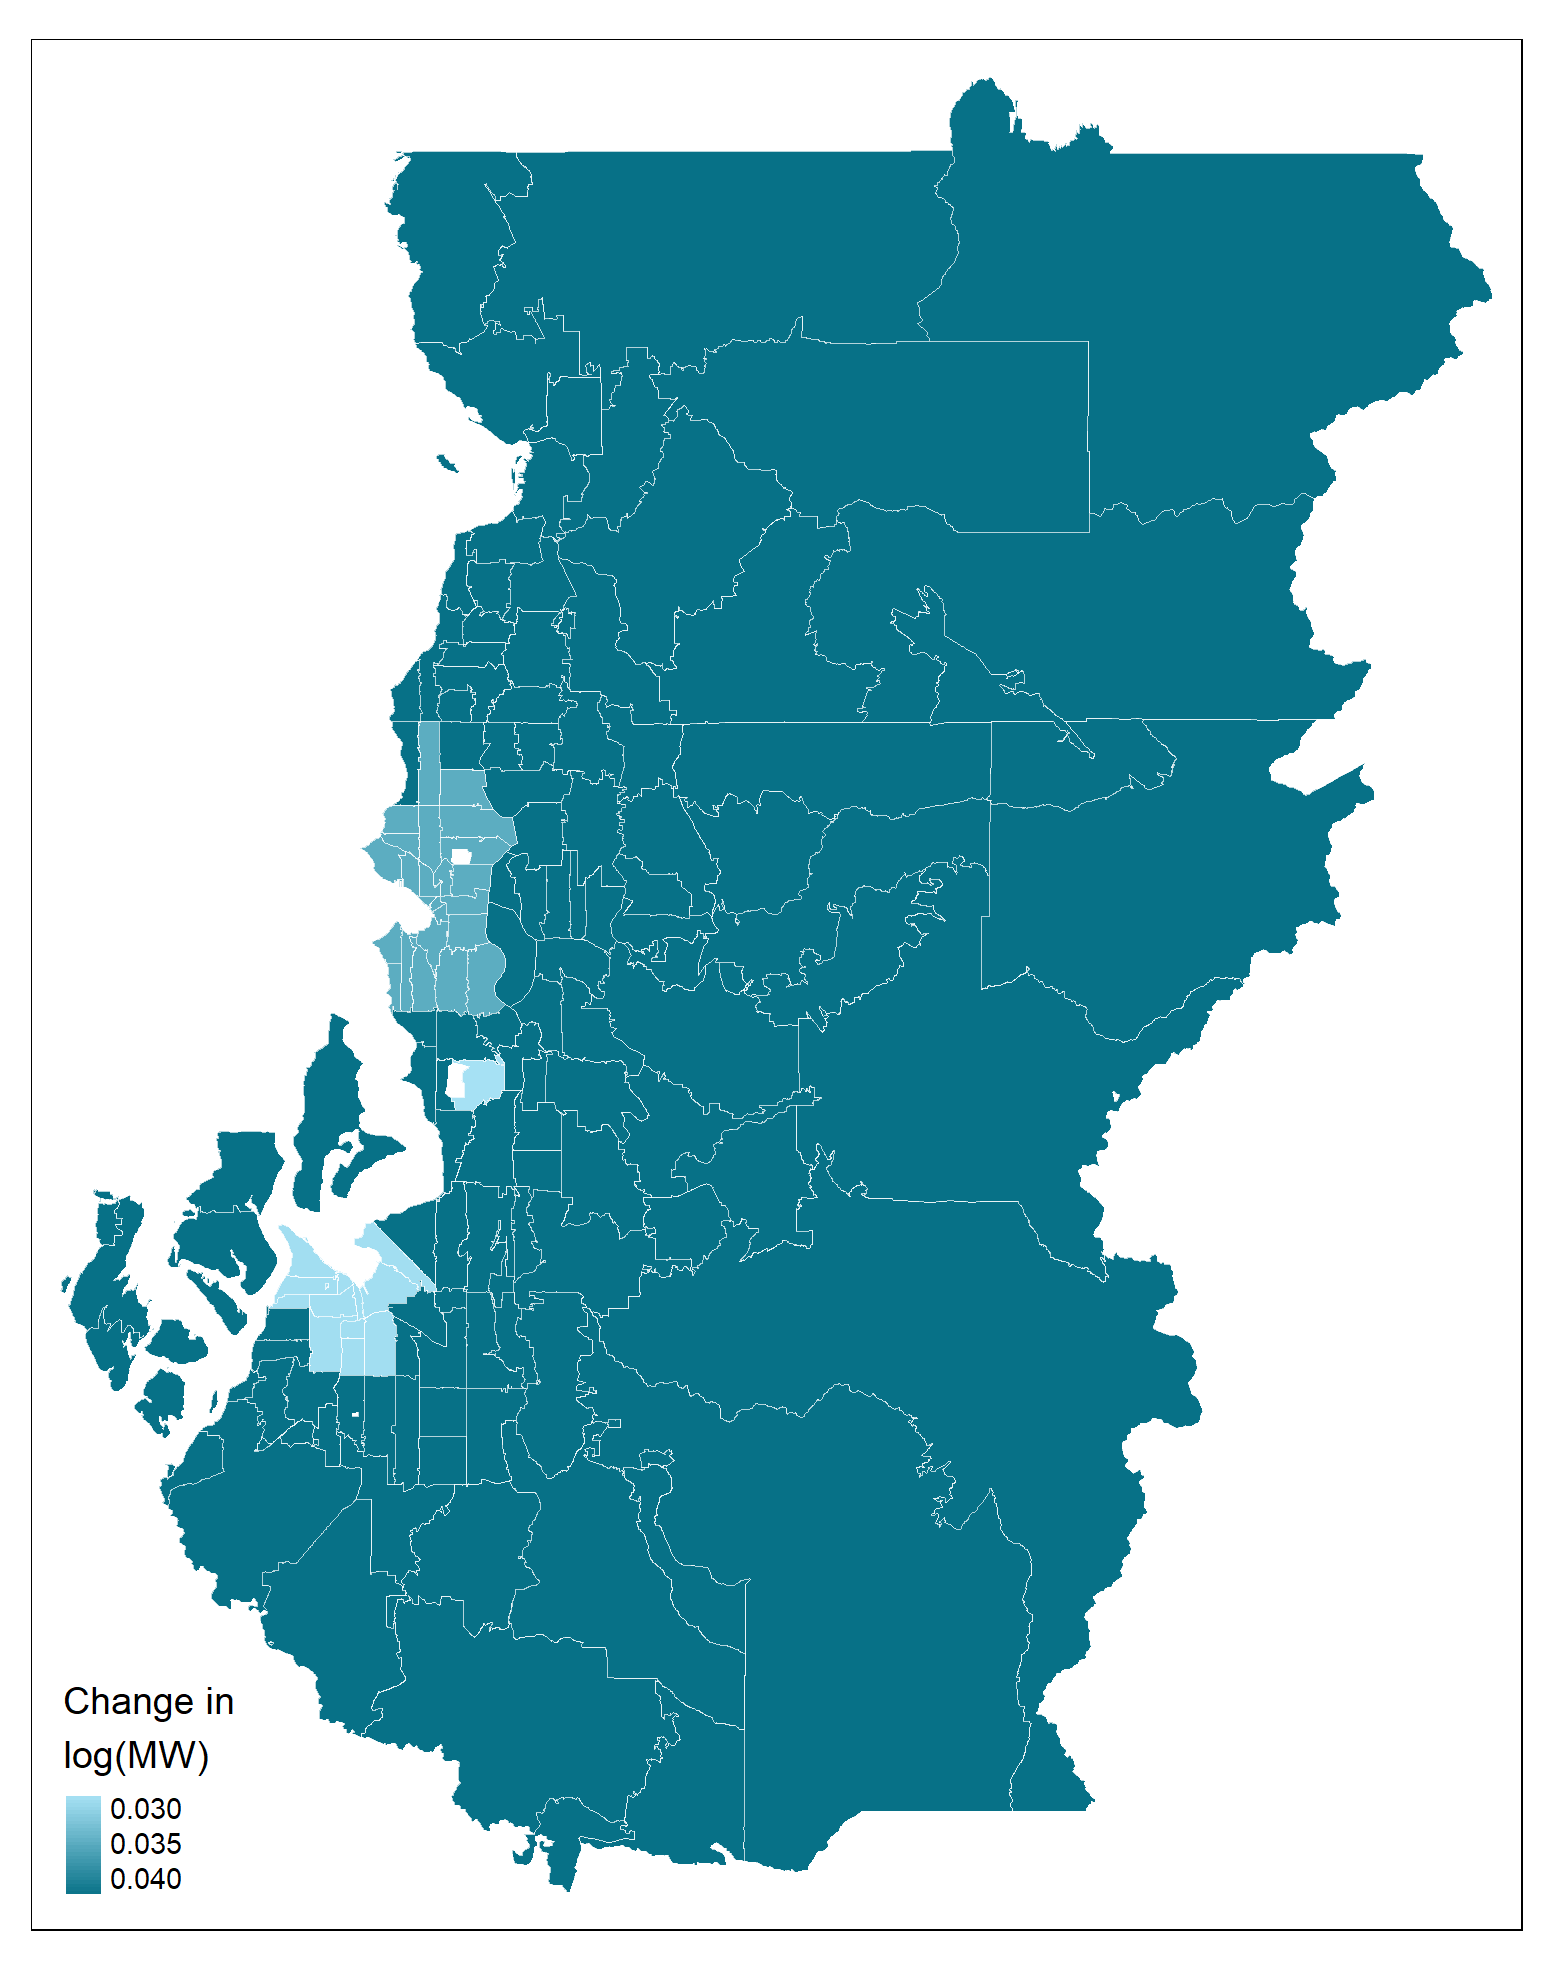
\includegraphics[scale = 0.36]{maps_events/output/seattle_2018-12_actual_mw.png}
            \end{figure}   
        \end{column}
        \begin{column}{0.50\textwidth}
            \vspace{-4mm}
            \begin{figure}
                \centering
                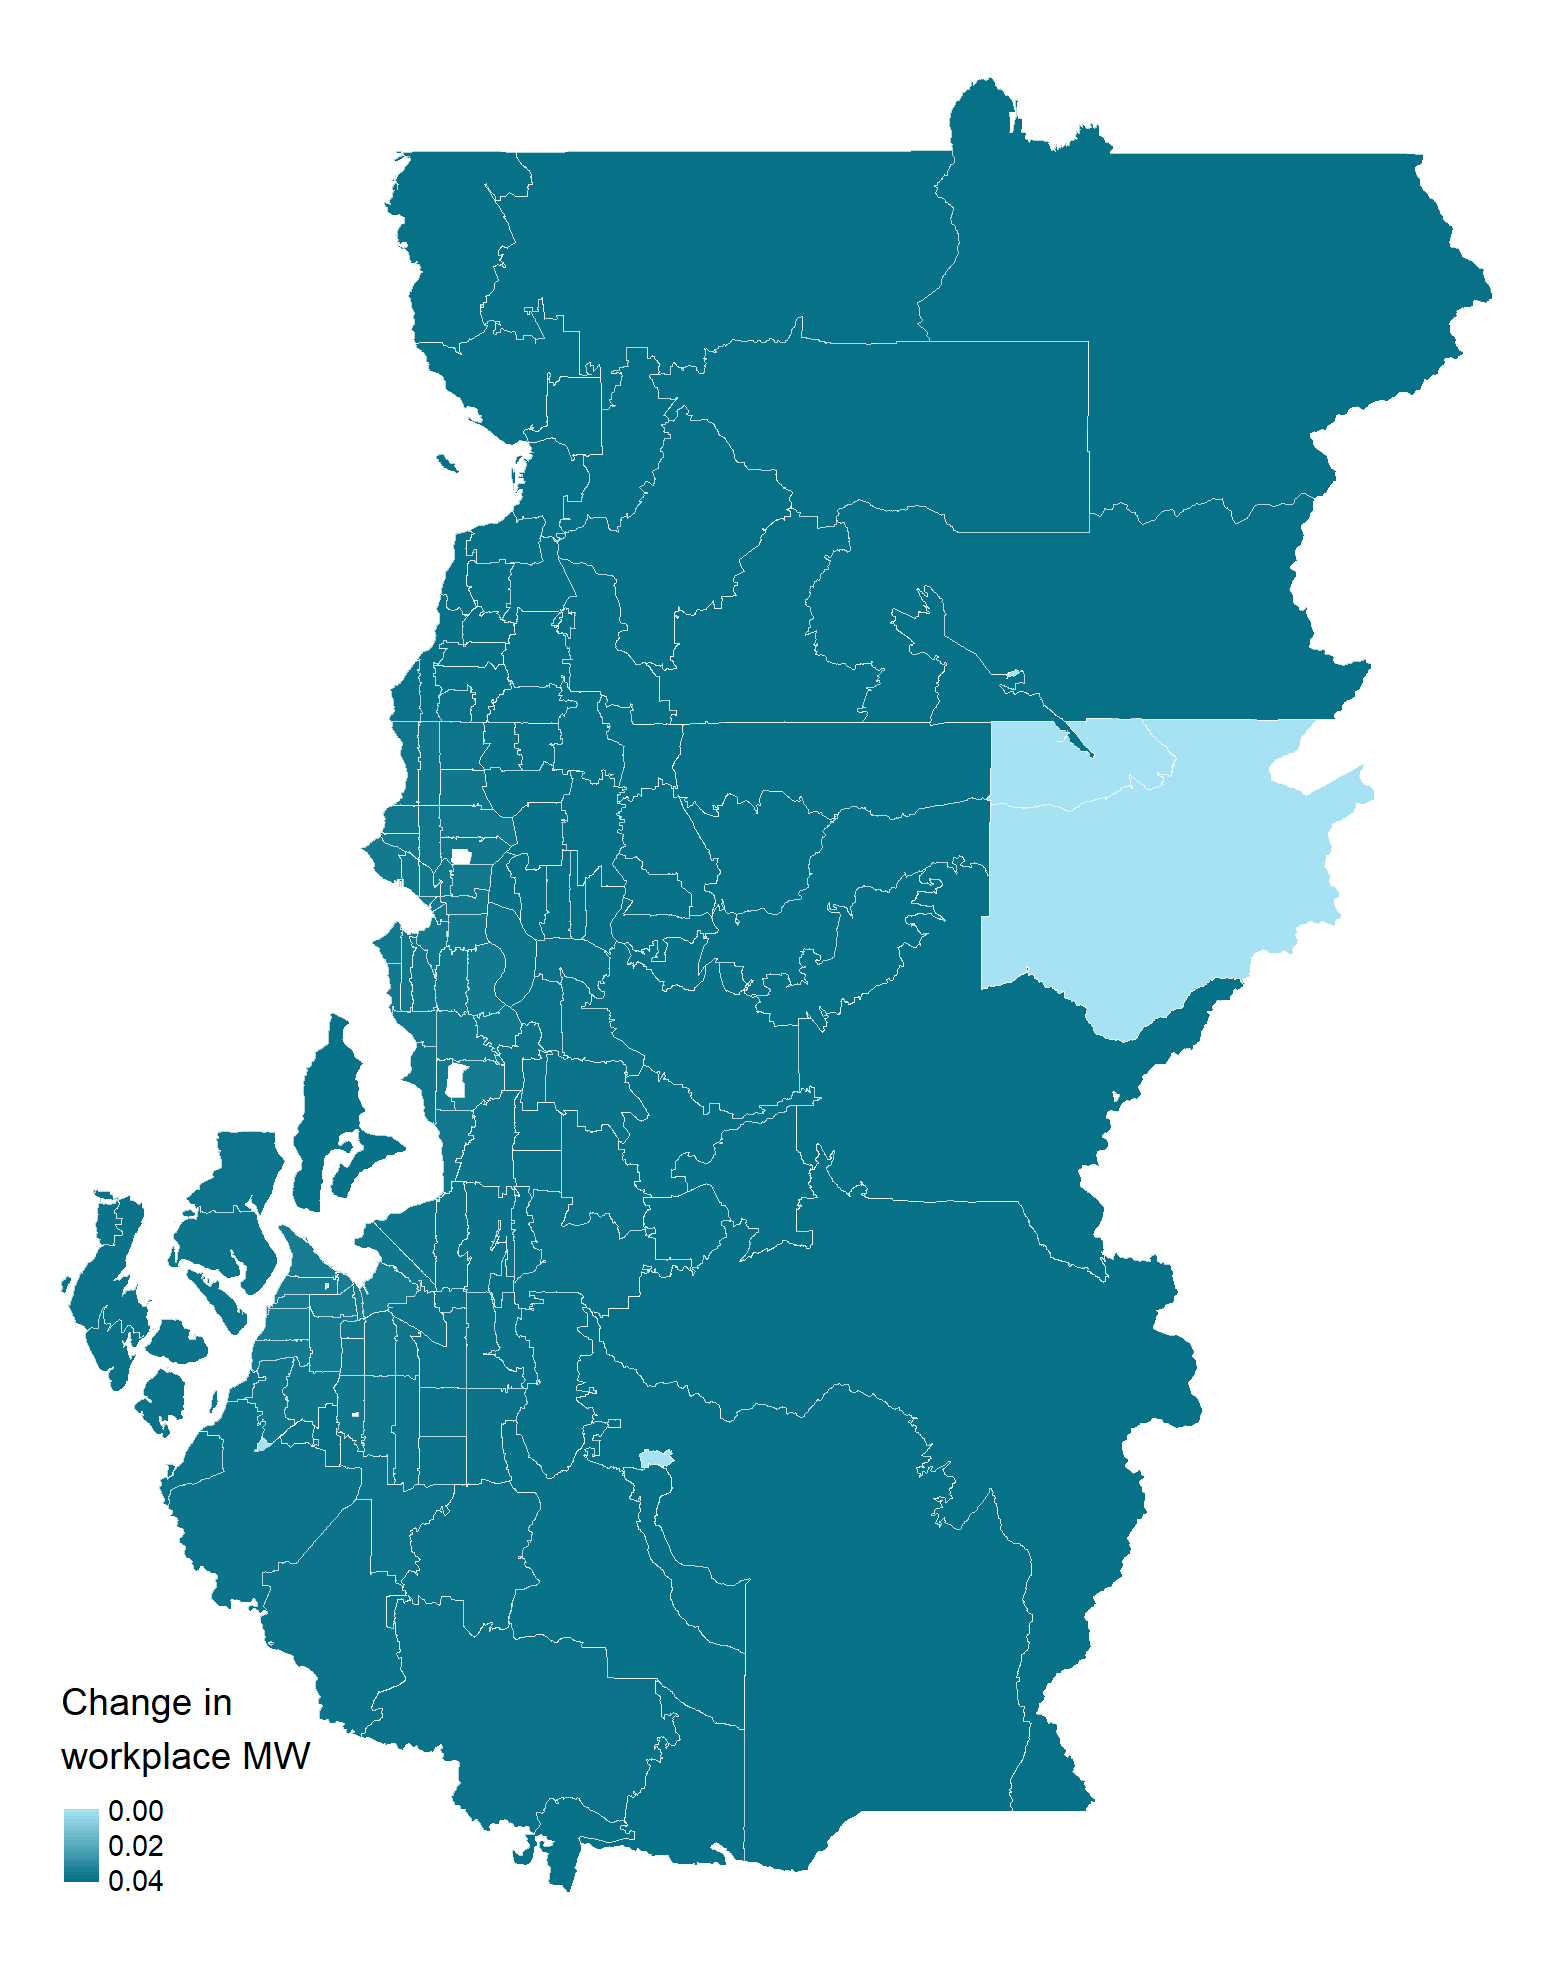
\includegraphics[scale = 0.36]{maps_events/output/seattle2018-12_exp_mw.png}
            \end{figure}   
        \end{column}
    \end{columns}
     \hyperlink{chi_example}{\beamerbutton{Go back}}
\end{frame}

\begin{frame}[label = san_diego_example]
\frametitle{San Diego (MW changes in January 2019)}
    \begin{columns}
        \begin{column}{0.50\textwidth}
            \vspace{-4mm}
            \begin{figure}
                \centering
                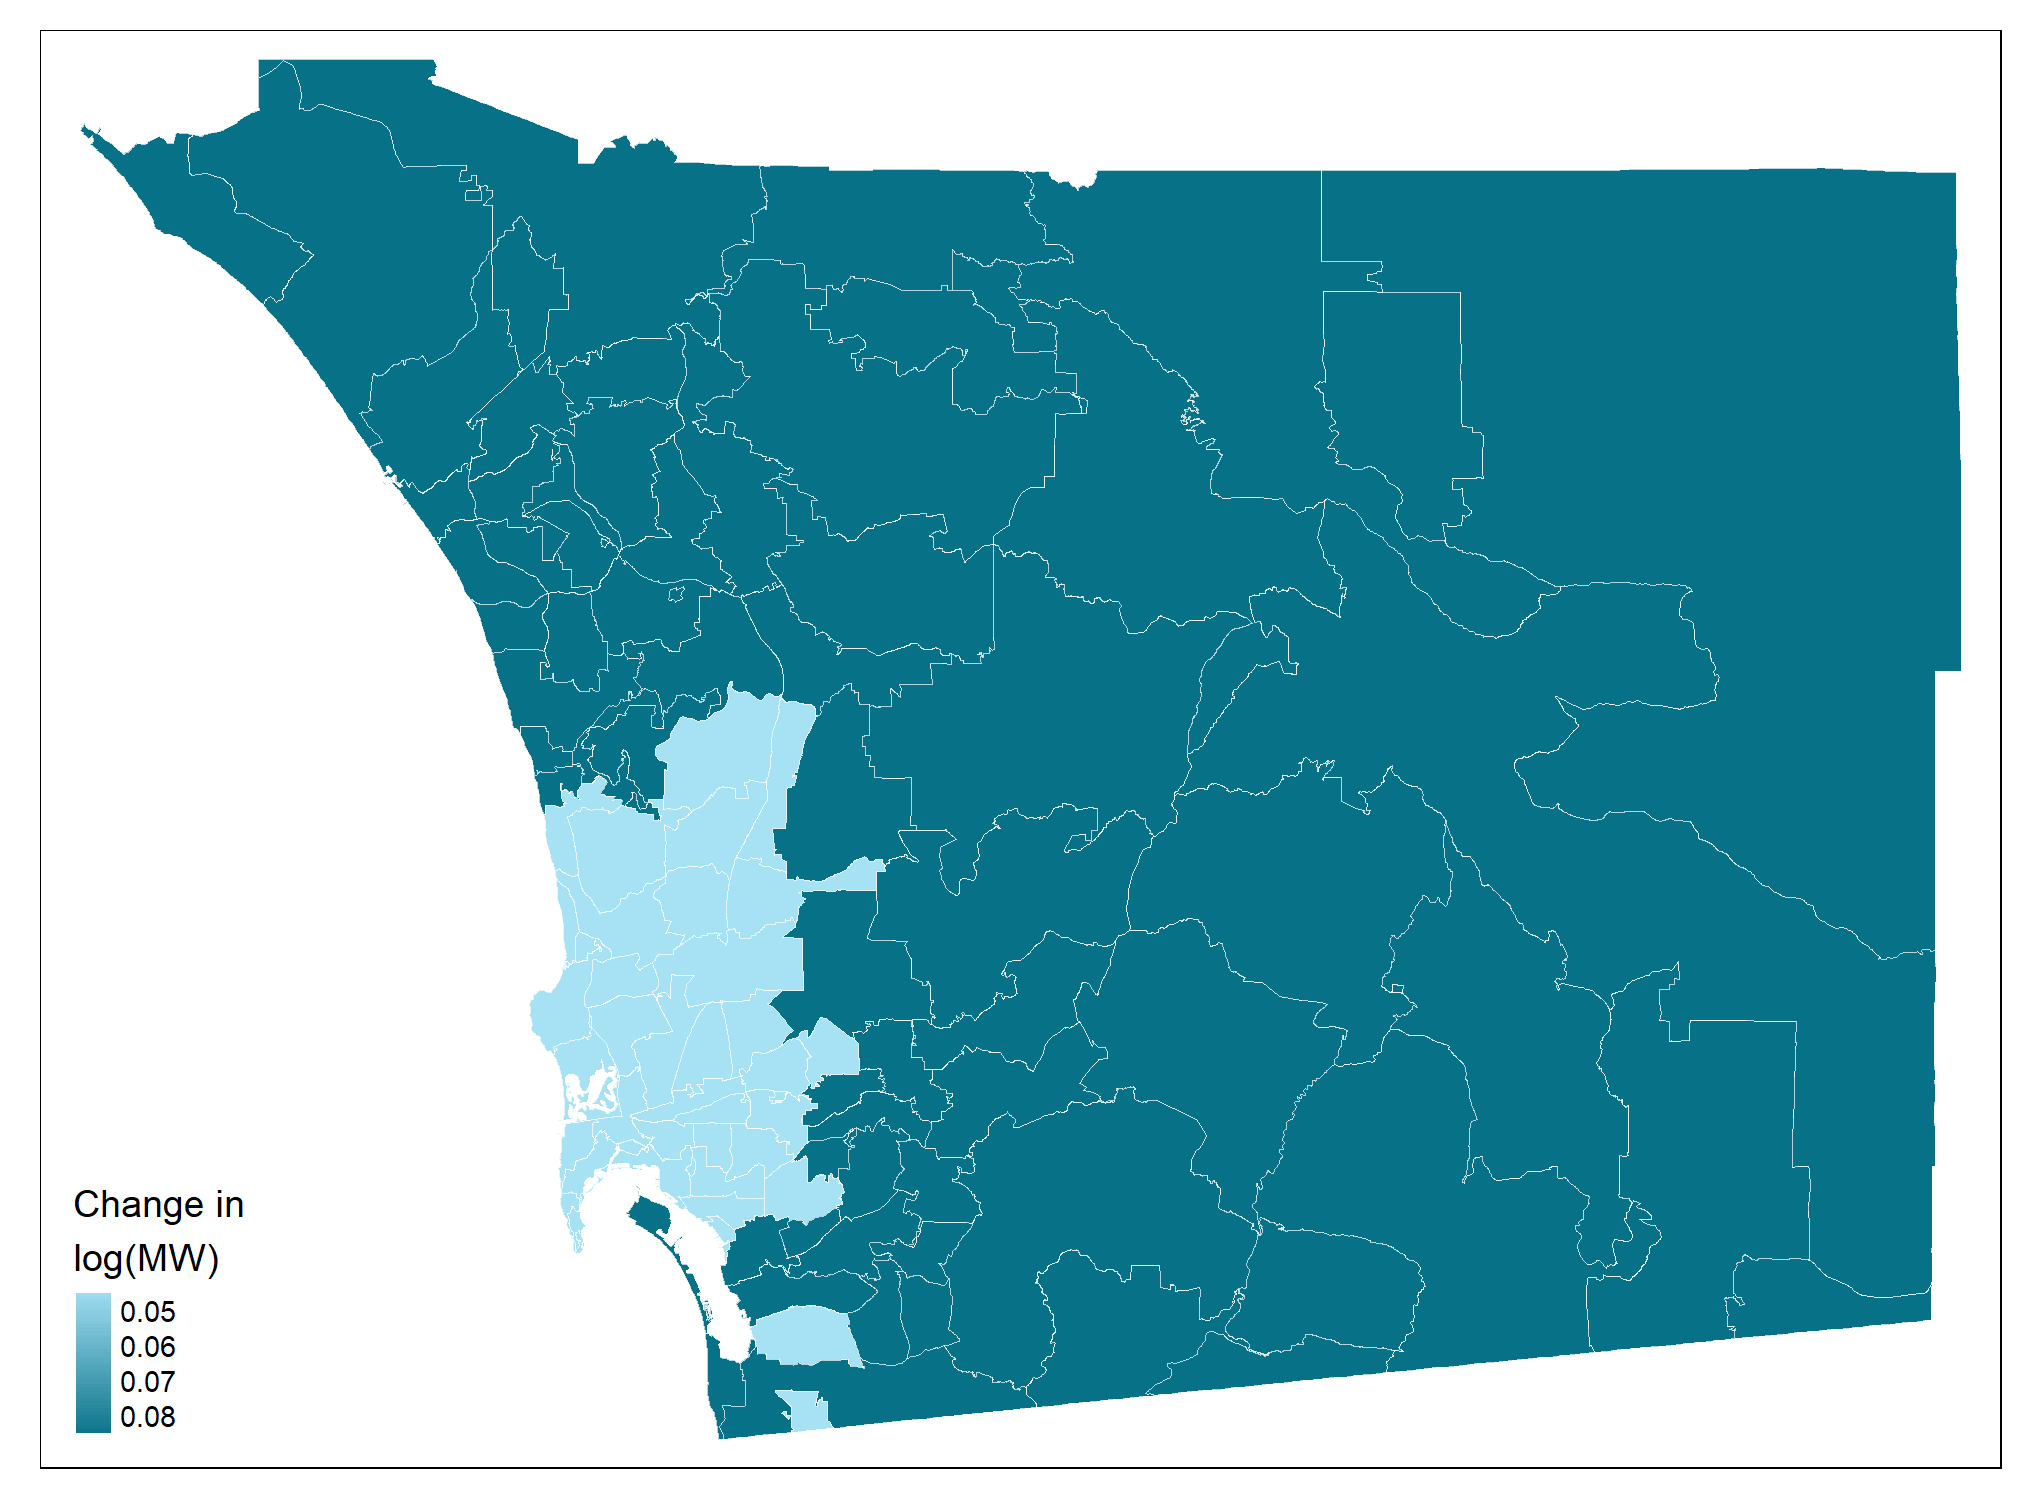
\includegraphics[scale = 0.36]{maps_events/output/san_diego_2018-12_actual_mw.png}
            \end{figure}   
        \end{column}
        \begin{column}{0.50\textwidth}
            \vspace{-4mm}
            \begin{figure}
                \centering
                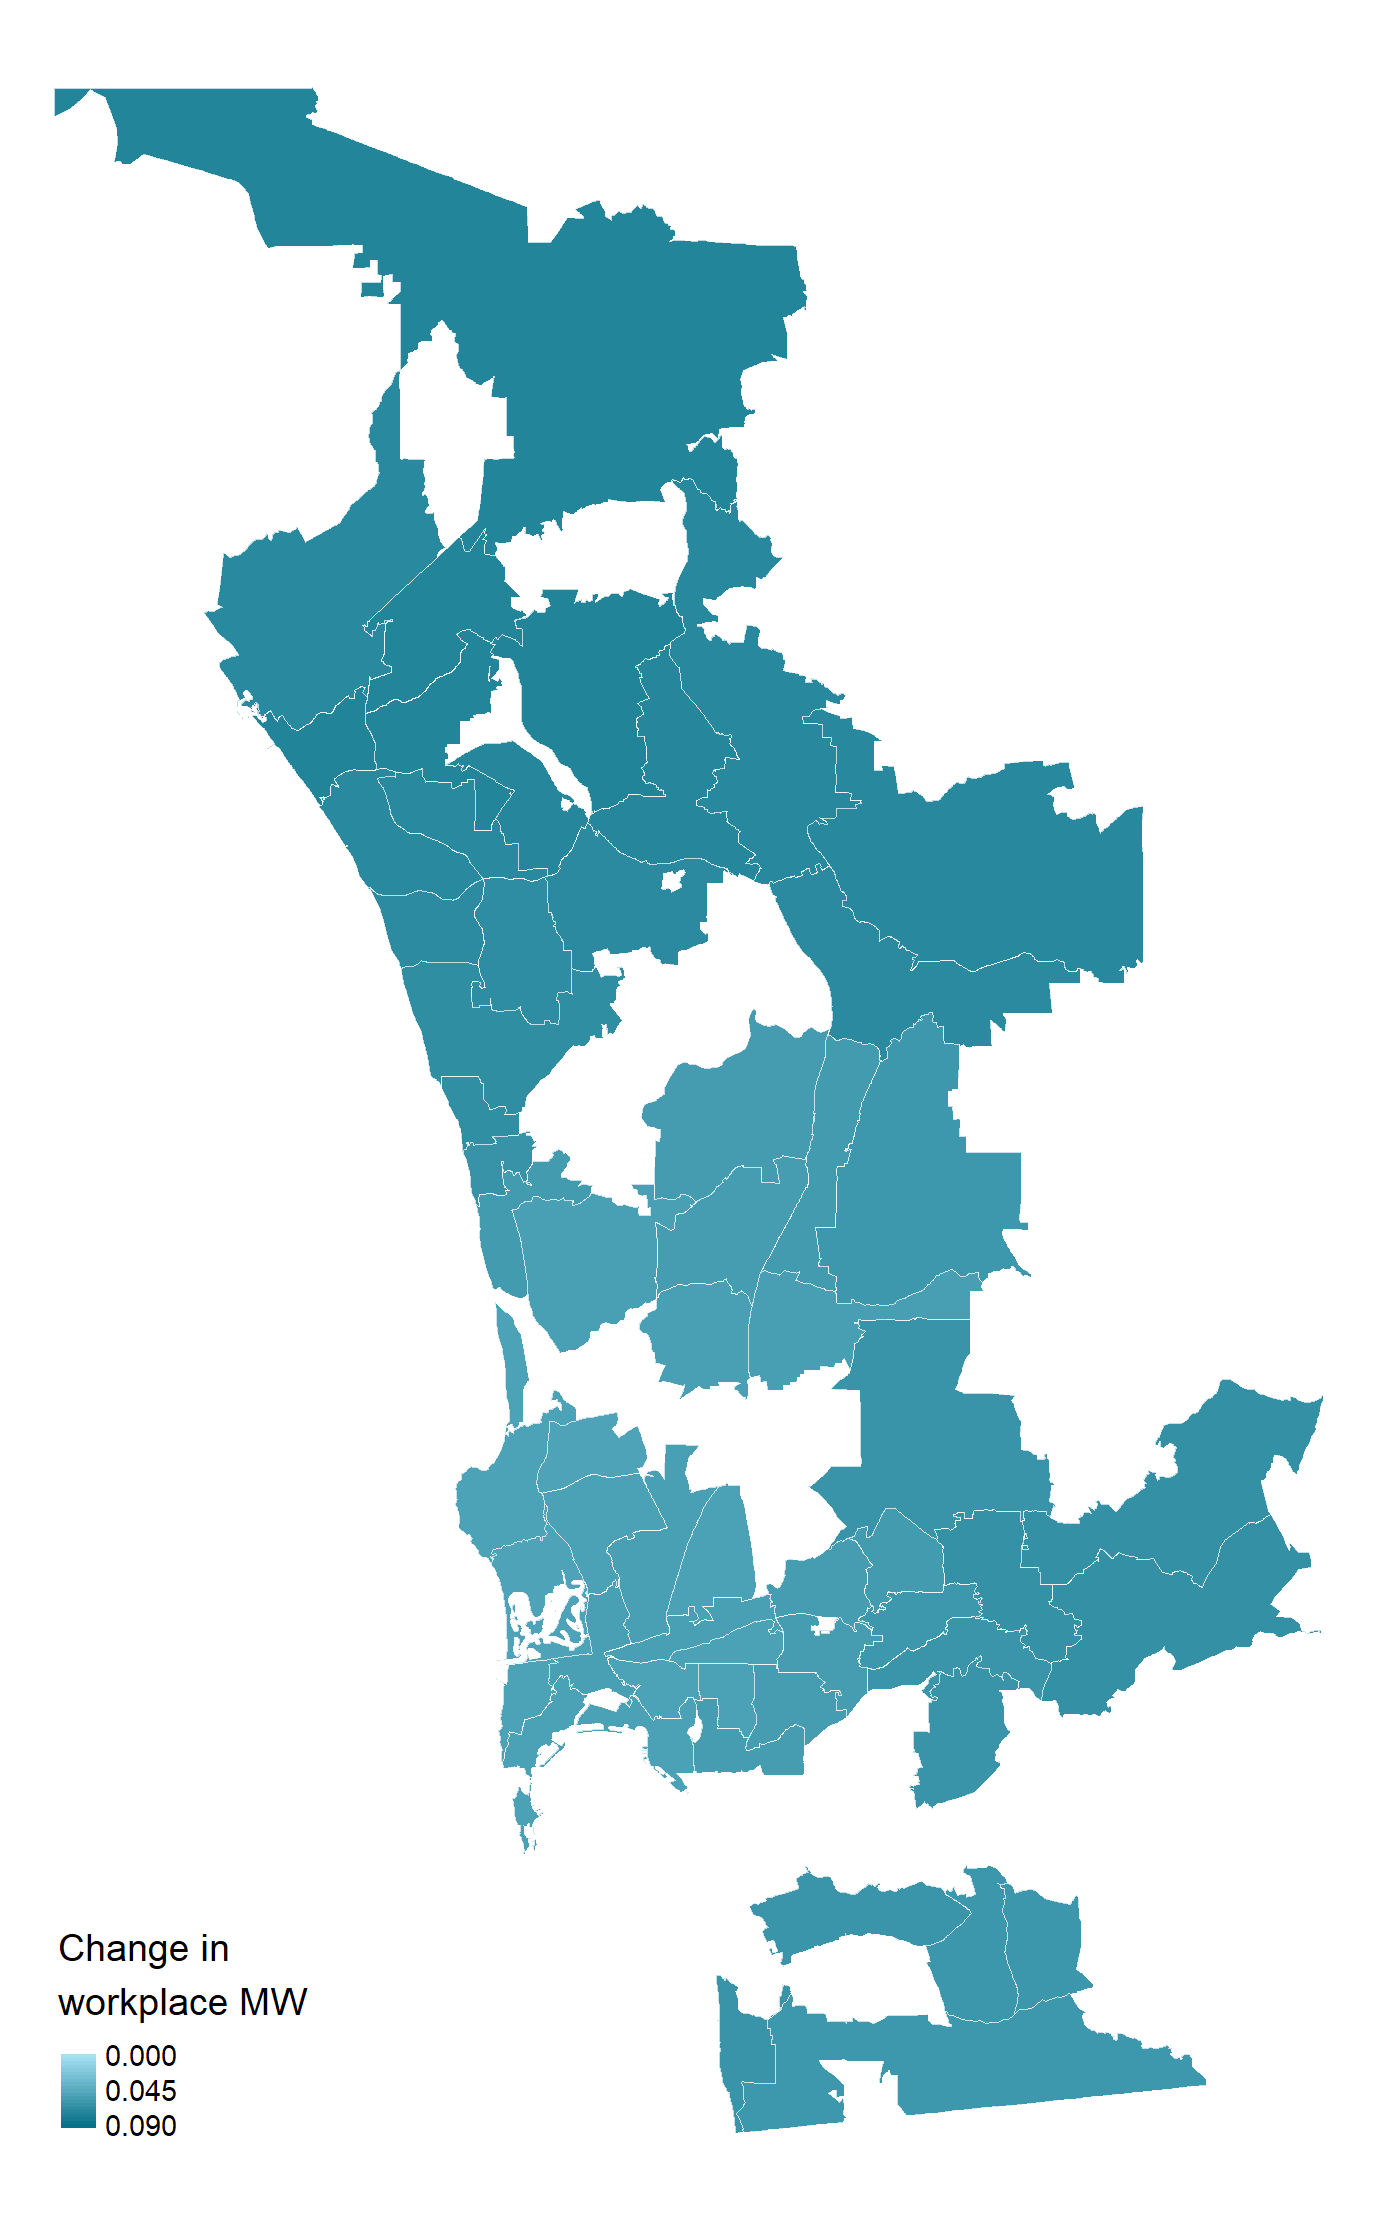
\includegraphics[scale = 0.36]{maps_events/output/san_diego2018-12_exp_mw.png}
            \end{figure}   
        \end{column}
    \end{columns}
     \hyperlink{chi_example}{\beamerbutton{Go back}}
\end{frame}

\begin{frame}[label = kc_example]
\frametitle{Kansas City (MW changes in January 2019)}
    \begin{columns}
        \begin{column}{0.50\textwidth}
            \vspace{-4mm}
            \begin{figure}
                \centering
                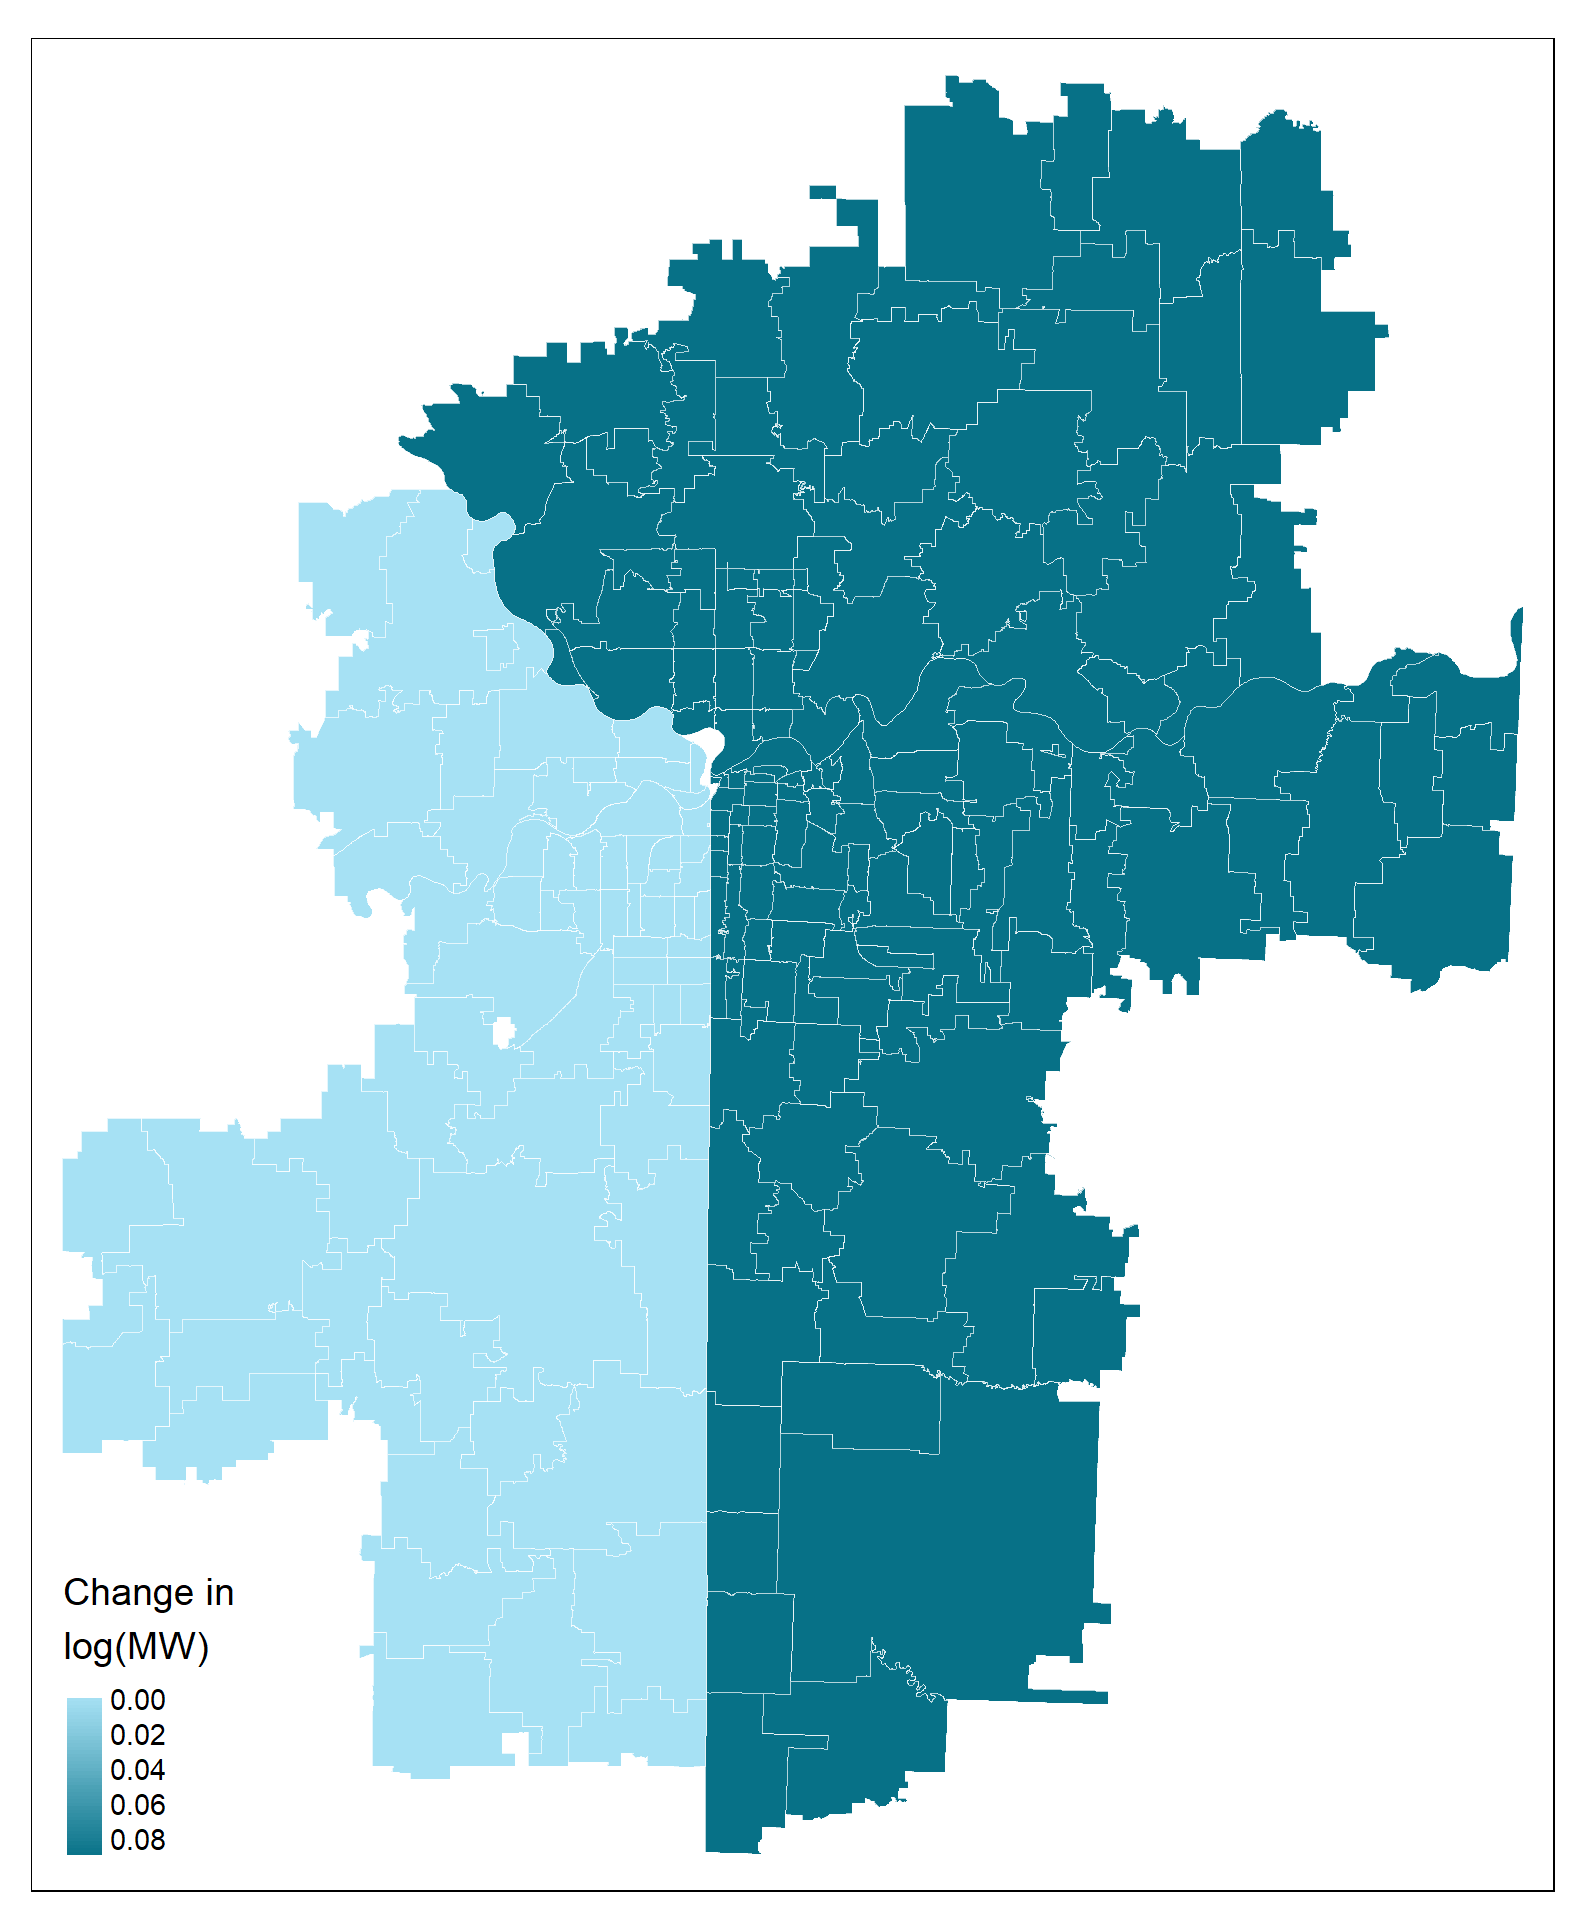
\includegraphics[scale = 0.36]{maps_events/output/kc_2018-12_actual_mw.png}
            \end{figure}   
        \end{column}
        \begin{column}{0.50\textwidth}
            \vspace{-4mm}
            \begin{figure}
                \centering
                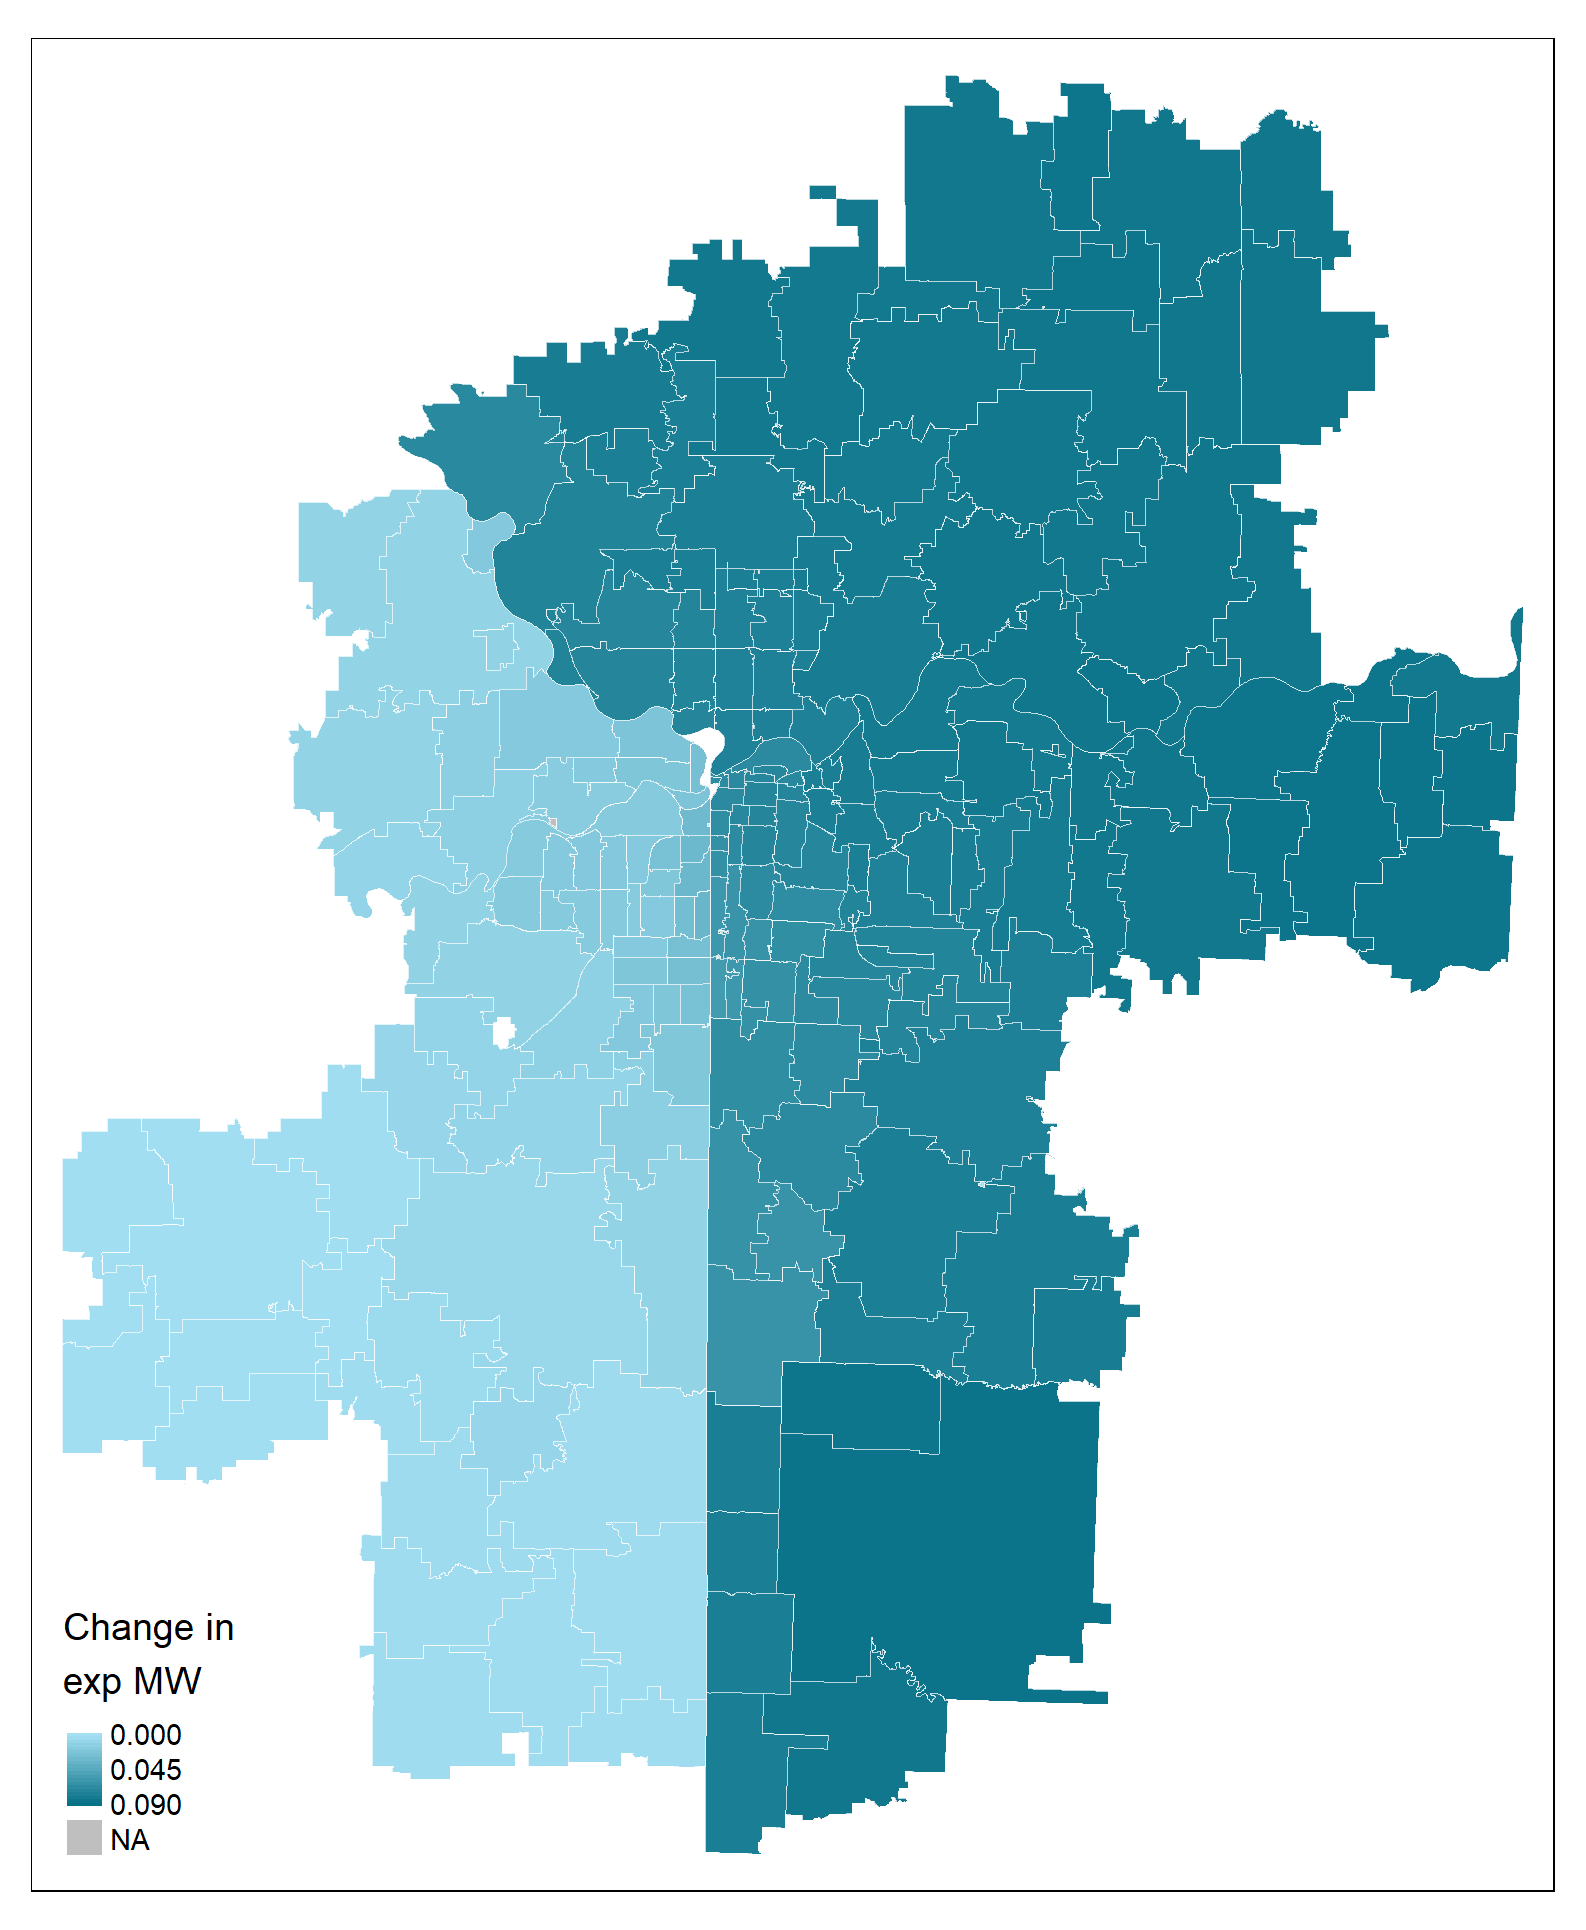
\includegraphics[scale = 0.36]{maps_events/output/kc2018-12_exp_mw.png}
            \end{figure}   
        \end{column}
    \end{columns}
     \hyperlink{chi_example}{\beamerbutton{Go back}}
\end{frame}

\begin{frame}[label = microfound]
	\frametitle{Microfoundation}
	Say a representative $(i,z)$ worker chooses between housing demand $h_{iz}$,
	non-tradable consumption $c^{\text{NT}}_{iz}$, and tradable consumption $c^{\text{T}}_{iz}$,
	by maximizing
	\[
	u_{iz} = u \left(h_{iz}, c^{\text{NT}}_{iz}, c^{\text{T}}_{iz}\right)
	\]
	subject to

	\[
	r_i h_{iz} + p_i(\MW_i) c^{\text{NT}}_{iz} + c^{\text{T}}_{iz} \leq y_{iz}(\MW_z)
	\]

	where 
	\begin{itemize}
		\item $p_i(\MW_i)$ gives the price of local consumption, increasing in residence MW;
		\item the price of tradable consumption is normalized to one;  
		\item $y_{iz}(\MW_z)$ is an income function that depends positively on the workplace MW.
	\end{itemize}
\end{frame}

\begin{frame}
	\frametitle{Microfoundation (continuation)}

	Let $h_{iz}^*$ and $c_{iz}^*$ denote Marshallian demands, and 
	$\tilde h_{iz}^*$ denote the Hicksian housing demand.

	\vspace{2mm}

	By assumption, the price of the MW will increase prices of non-tradable consumption.
	Thus, consider the effect of an increase in $p_i$ on housing demand.
	The Slutsky equation implies that
	\[
	\frac{\partial h_{iz}^*}{\partial p_i} 
	= \frac{\partial \tilde h_{iz}^*}{\partial p_i} 
	- \frac{\partial h_{iz}^*}{\partial y_{iz}} c_{iz}^*
	\]

	Then, we have that 
	\[
	\frac{\partial h_{iz}^*}{\partial p_i} < 0 \iff 
	\frac{\partial \tilde h_{iz}^*}{\partial p_i} 
	< \frac{\partial h_{iz}^*}{\partial y_{iz}} c_{iz}^*
	\]

	\hyperlink{discuss4}{\beamerbutton{Go Back}}
\end{frame}

\begin{frame}[label = zillow_safmr]
	\frametitle{Comparison between Zillow and Small Area Fair Market Rents}
    \begin{figure}
    	\centering
	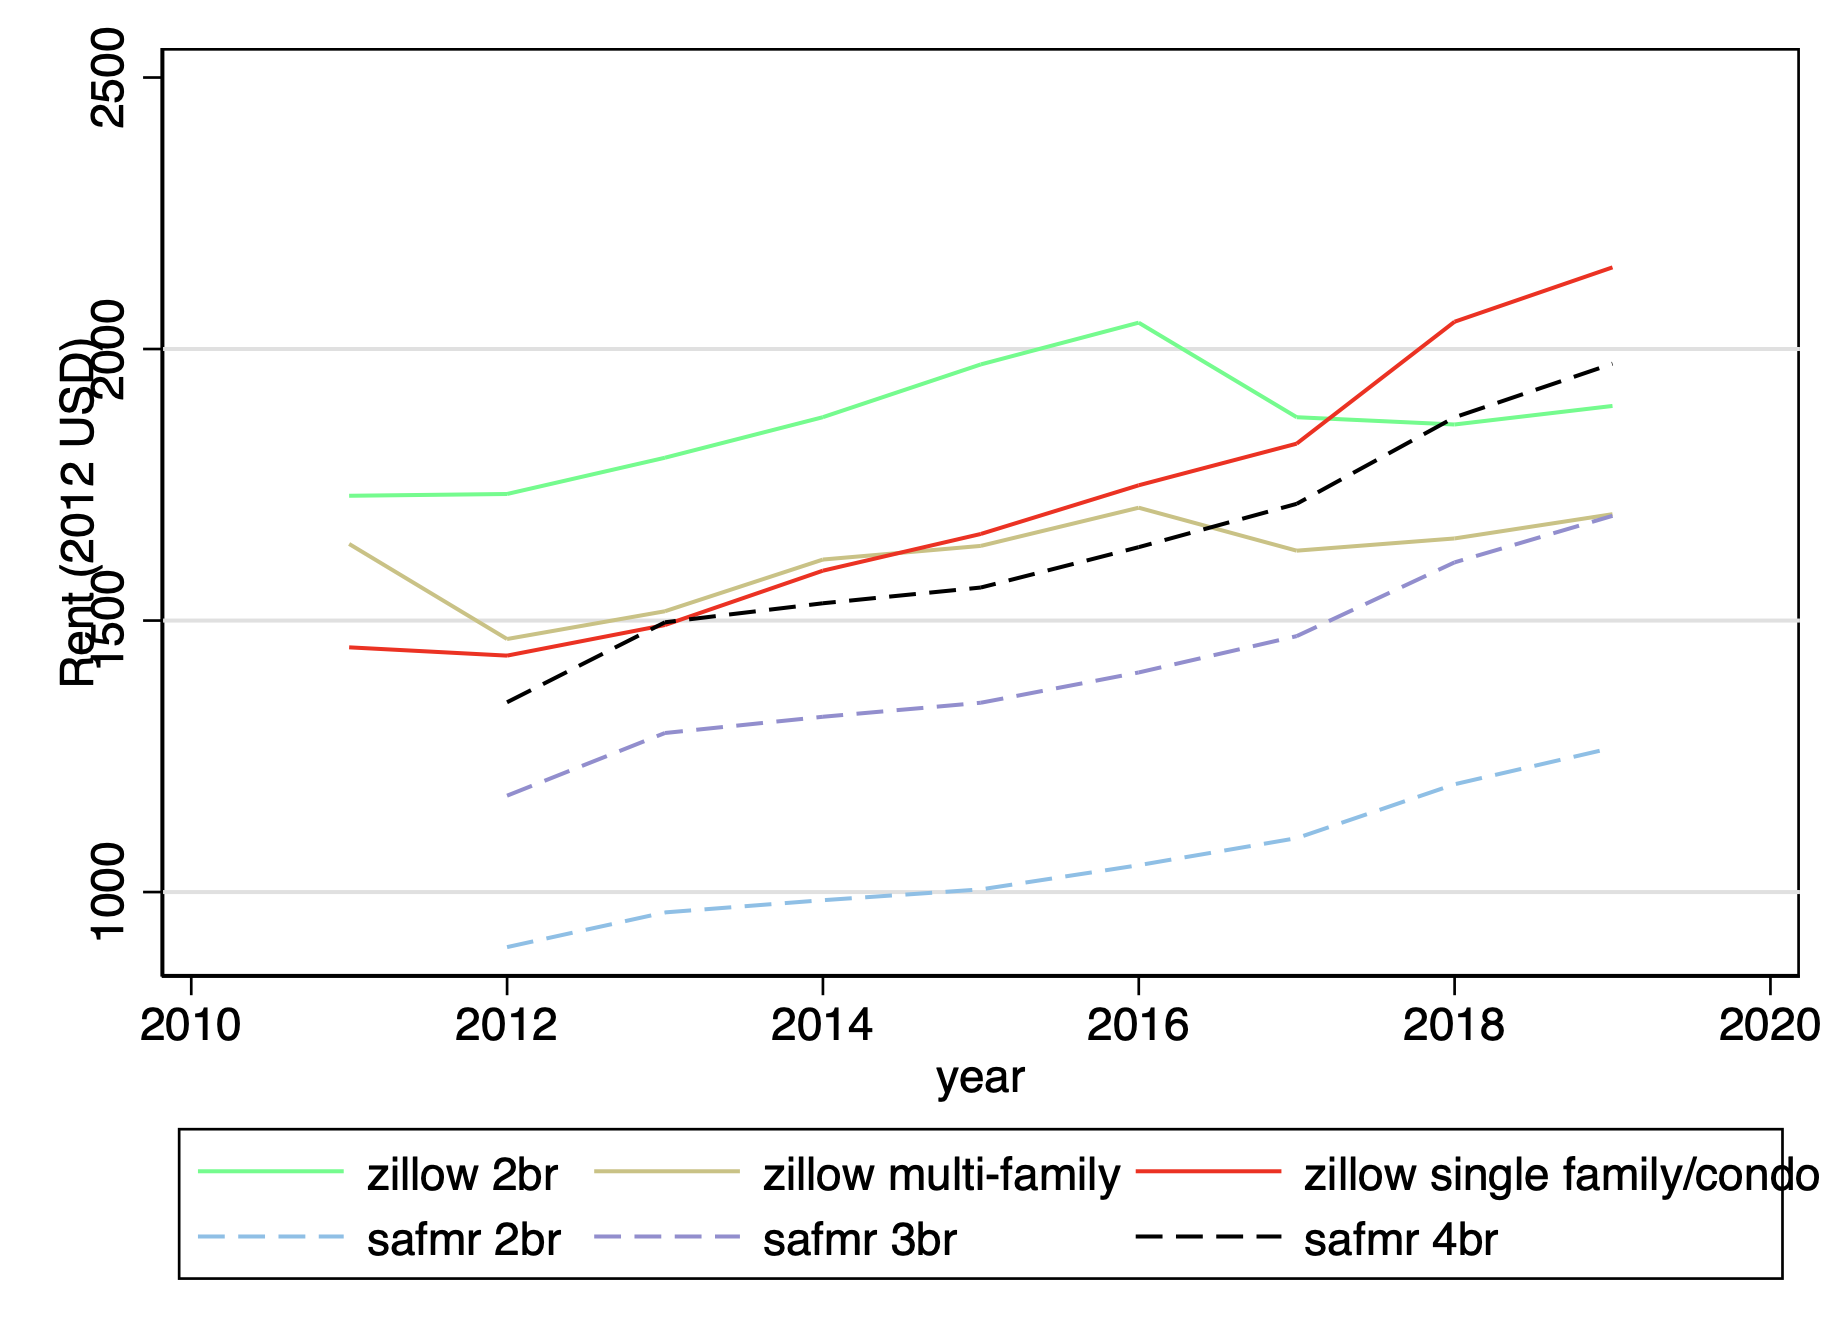
\includegraphics[scale = 0.32]{zillow_benchmark/output/trend_zillow_safmr_zipcode_m1.png}
    \end{figure}
	\hyperlink{zillow_data}{\beamerbutton{Go Back}}
\end{frame}

\begin{frame}[label = zillow_pop_density]
	\frametitle{Comparison between Zillow Sample and Population Density}
    \begin{figure}
    	\centering
	\vspace{10mm}
	\hspace{-23mm}
    	\begin{subfigure}{0.40\textwidth}
    		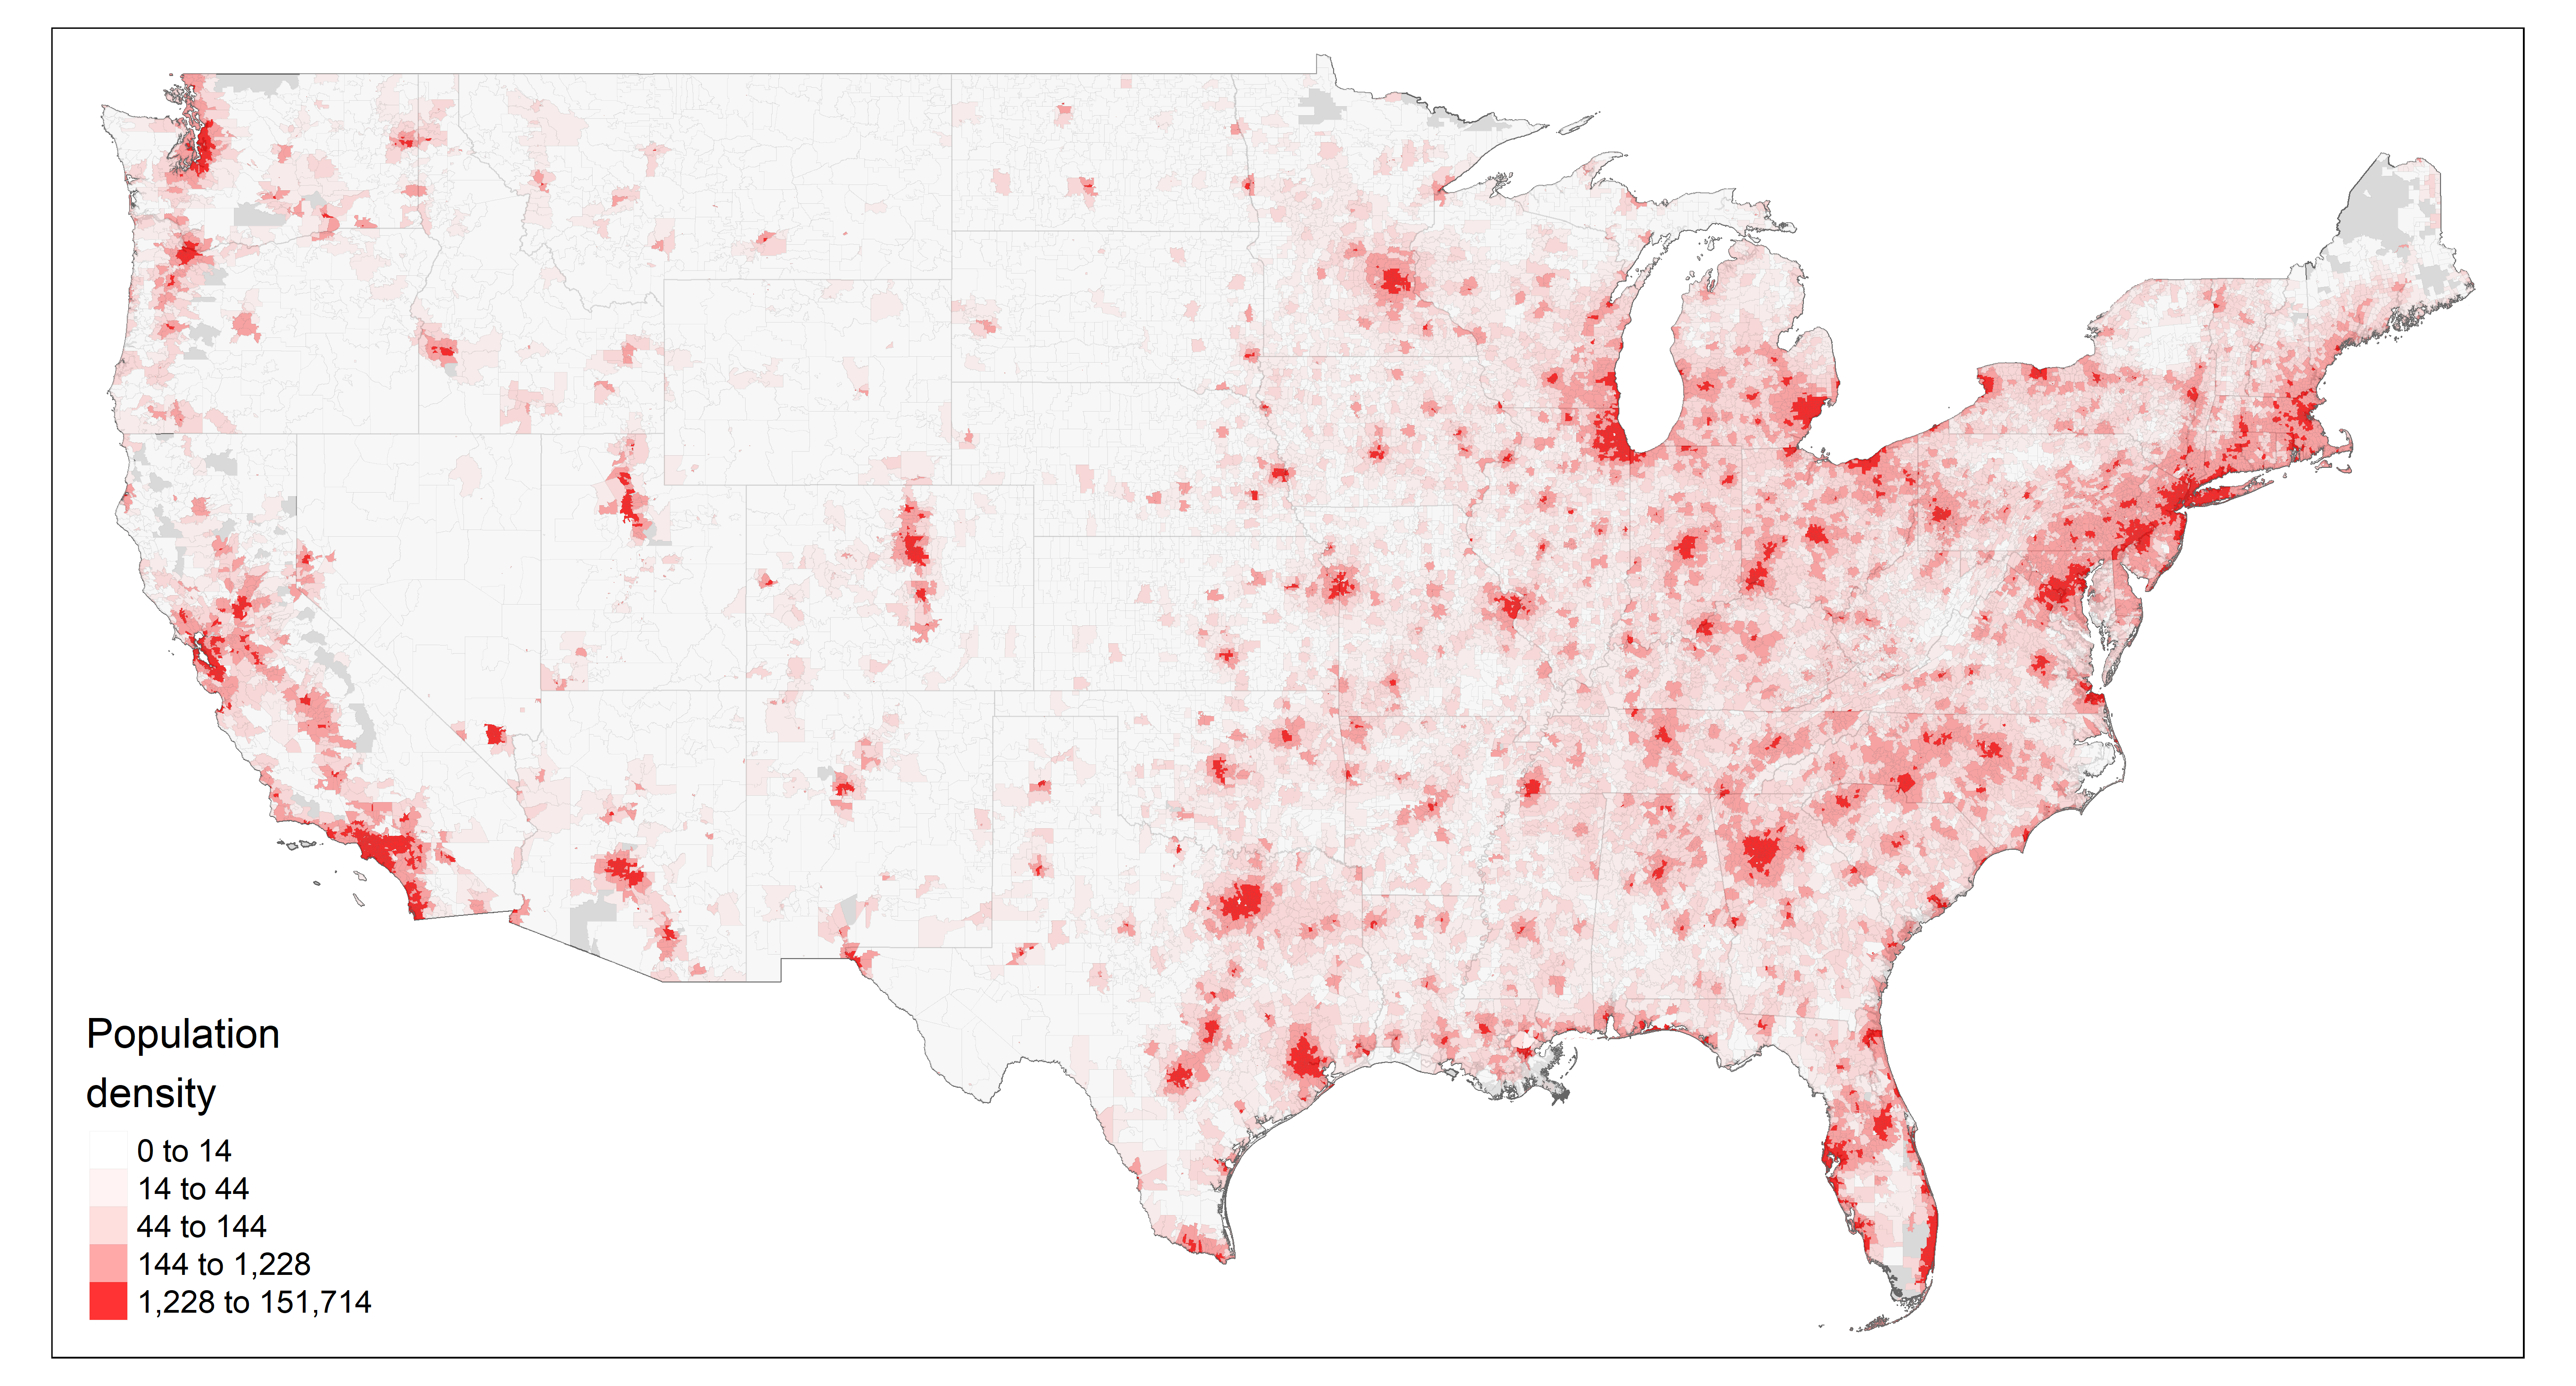
\includegraphics[scale = 0.32]{maps_US/output/USPS_zipcodes_pop_density.png}
    	\end{subfigure}%
	\quad\quad\quad\quad\quad\quad
        \begin{subfigure}{0.40\textwidth}
        	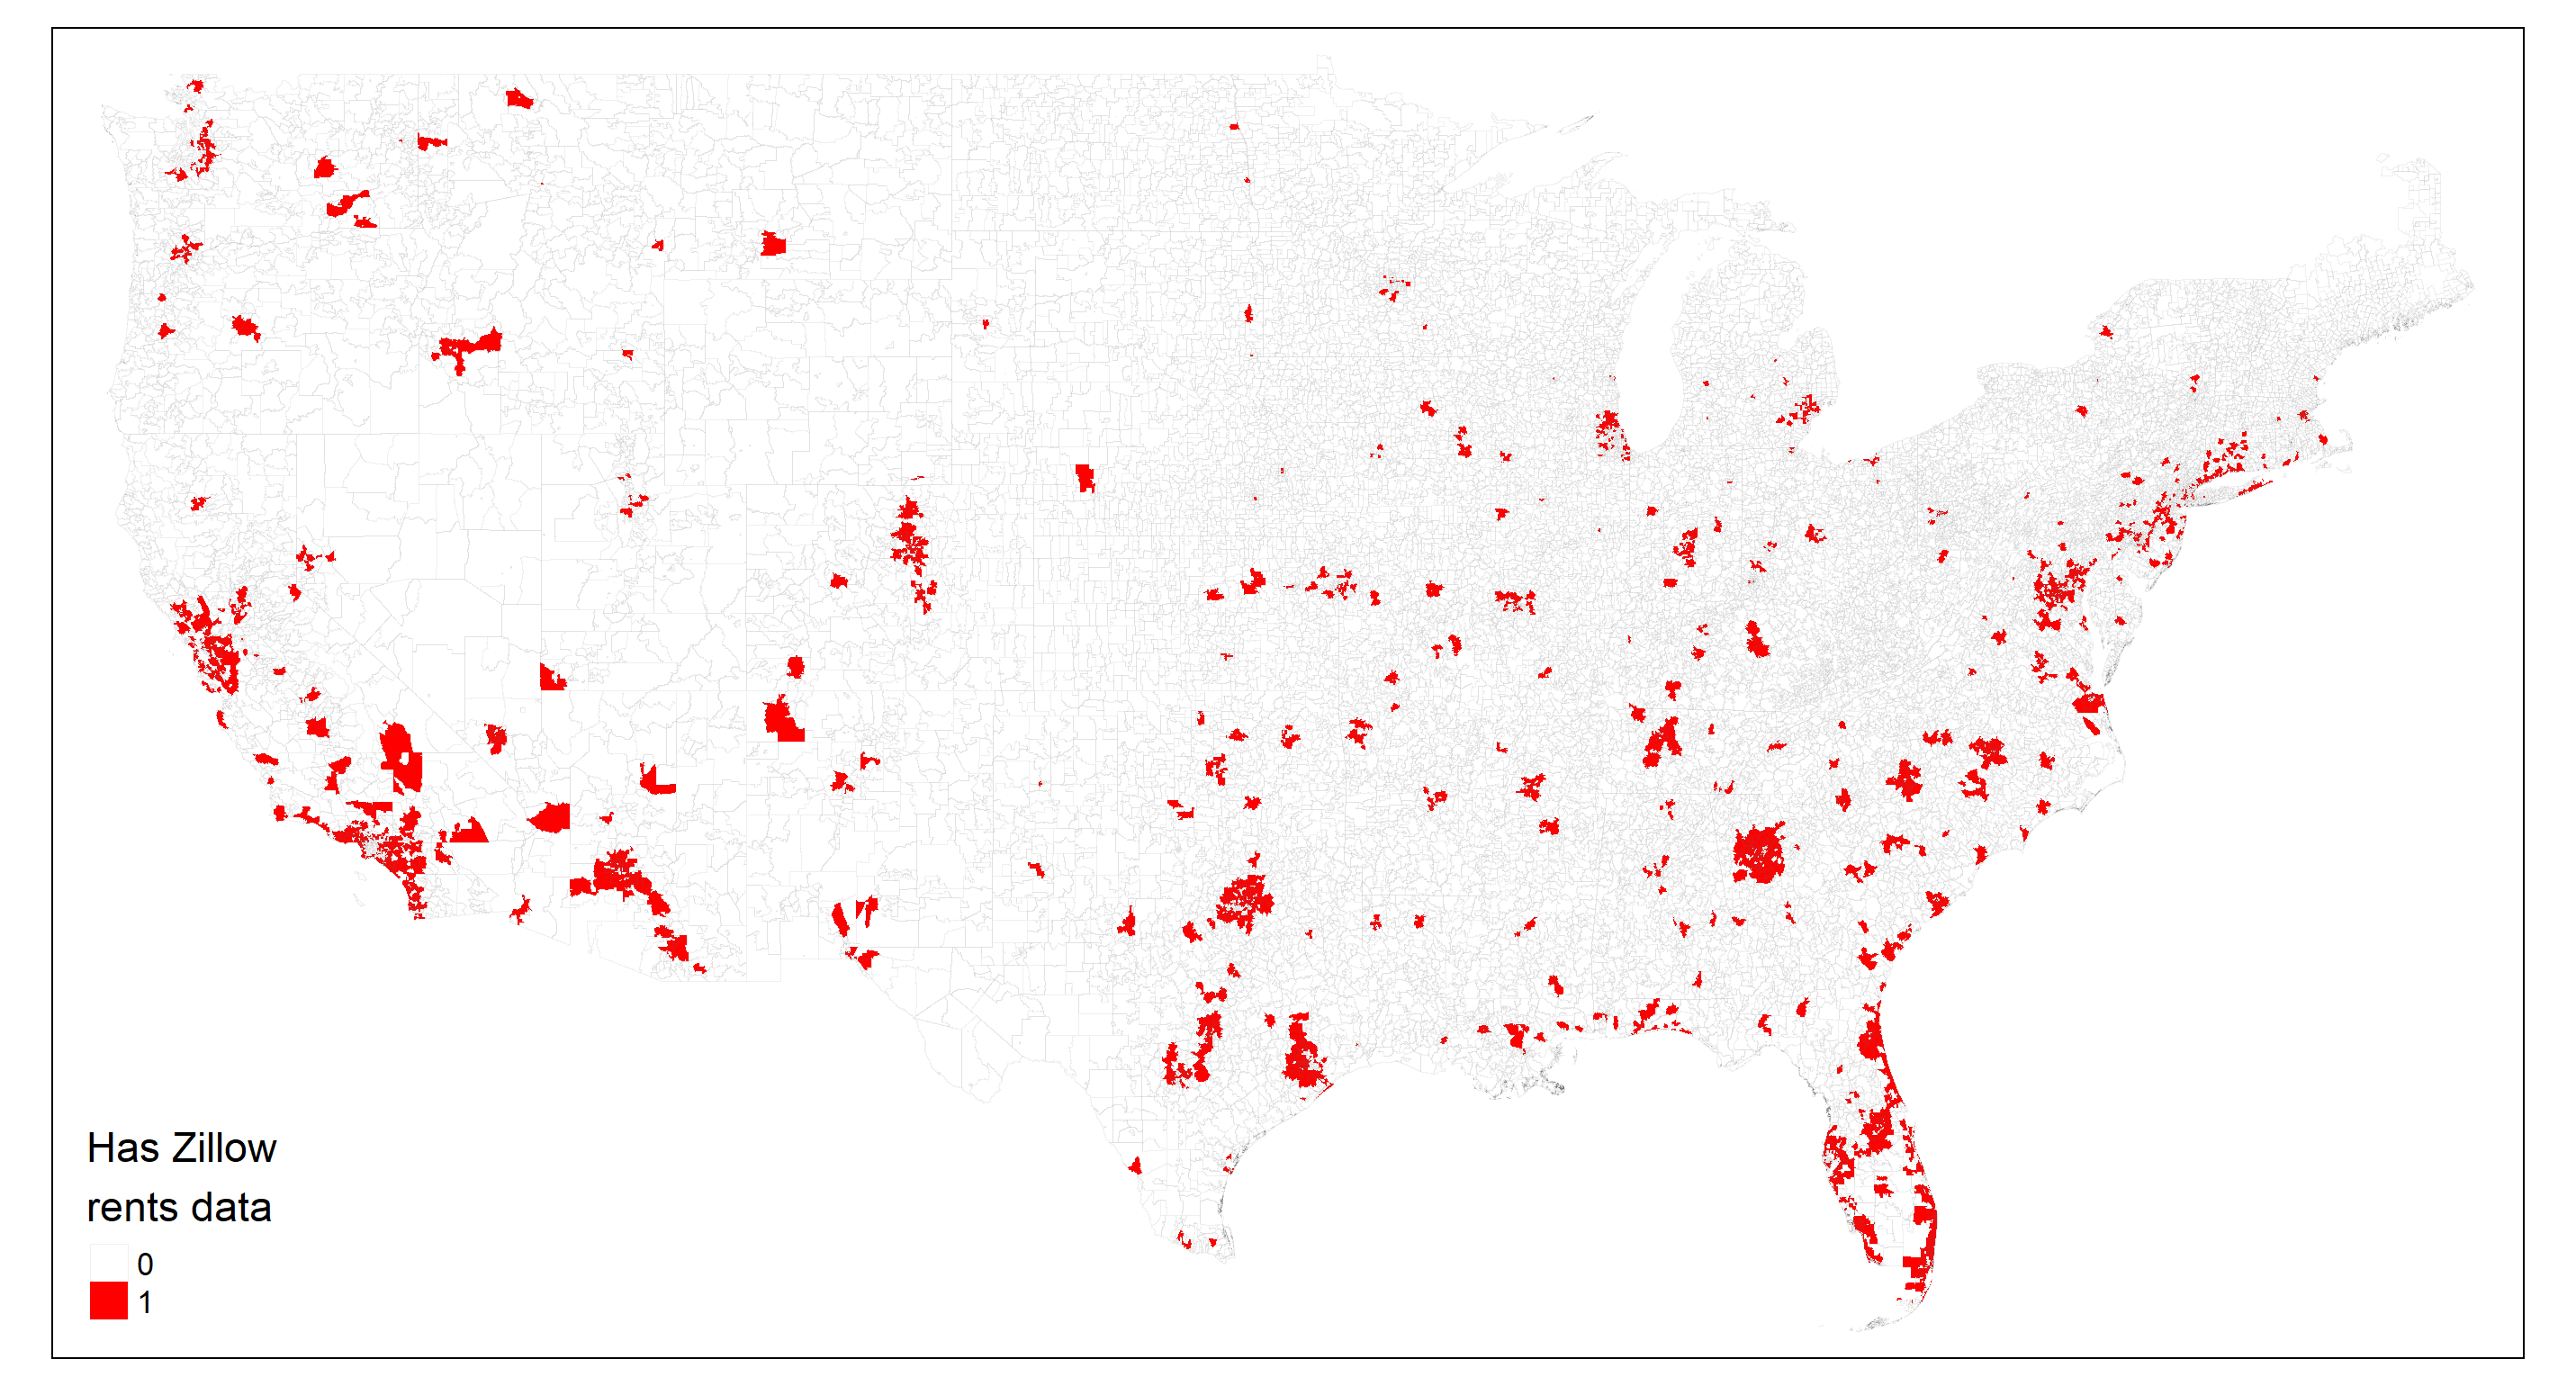
\includegraphics[scale = 0.32]{maps_US/output/USPS_zipcodes_zillow_data.png}
        \end{subfigure}
    \end{figure}
	\hyperlink{zillow_data}{\beamerbutton{Go Back}}
\end{frame}

\begin{frame}[label=dist_mw_changes]
	\frametitle{Distribution of (positive) MW changes}
	\begin{figure}
		\begin{subfigure}{0.49\textwidth}
			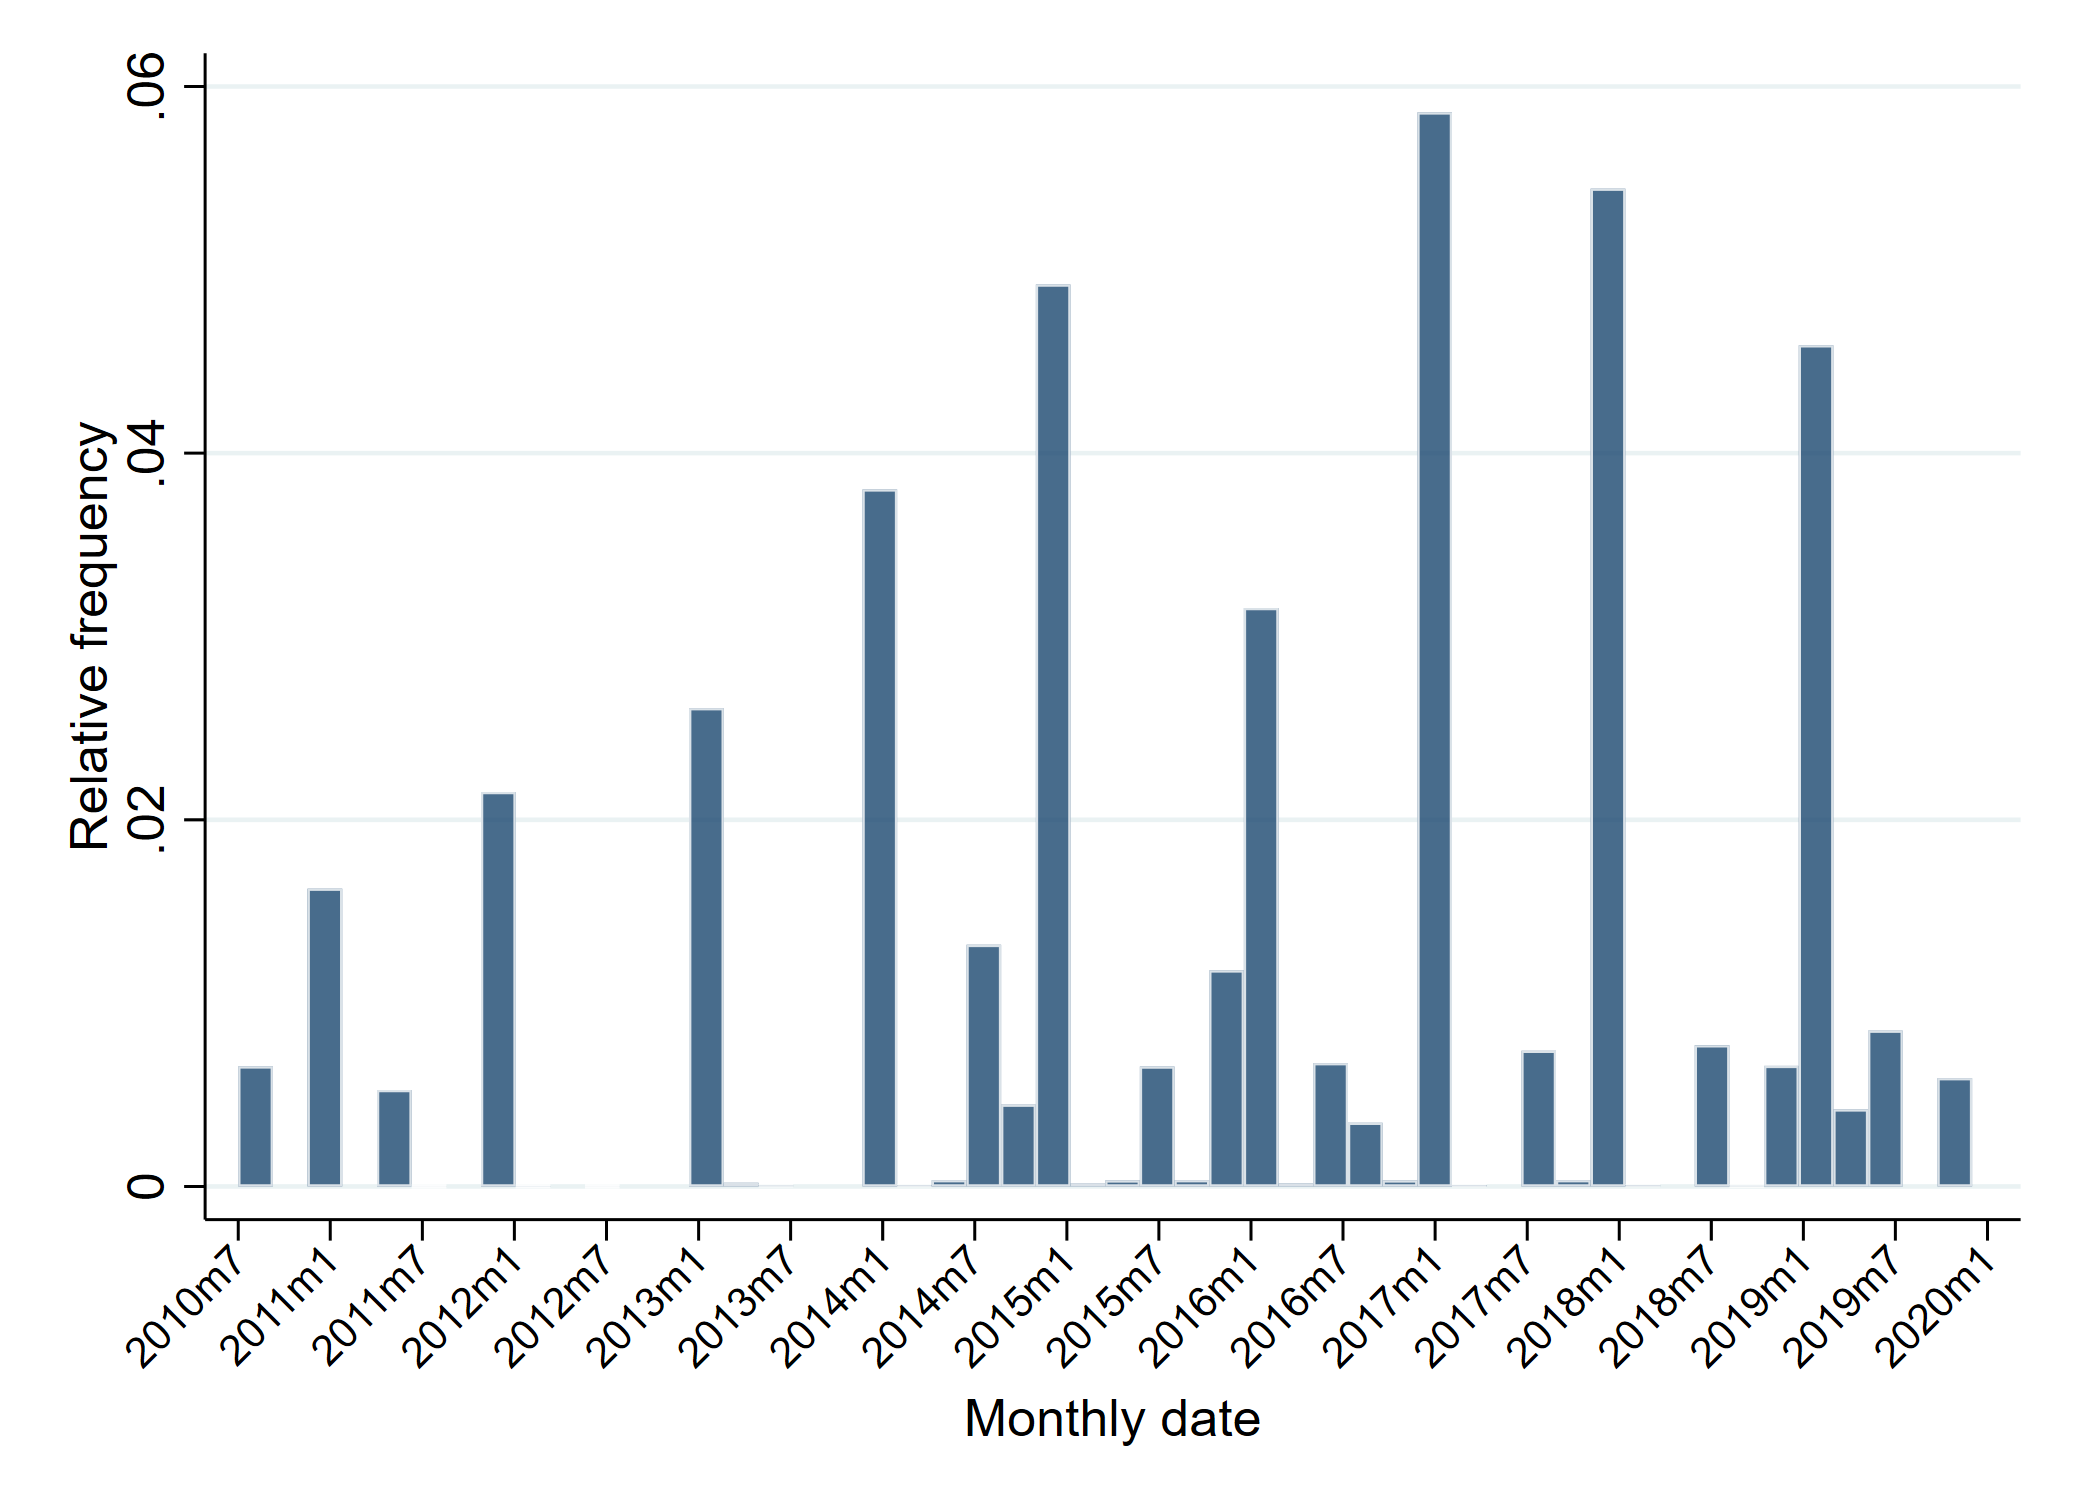
\includegraphics[width = 0.99\textwidth]{descriptive/estimation_samples/output/pct_ch_mw_date_dist.png}
		\end{subfigure}%
		\begin{subfigure}{0.49\textwidth}
			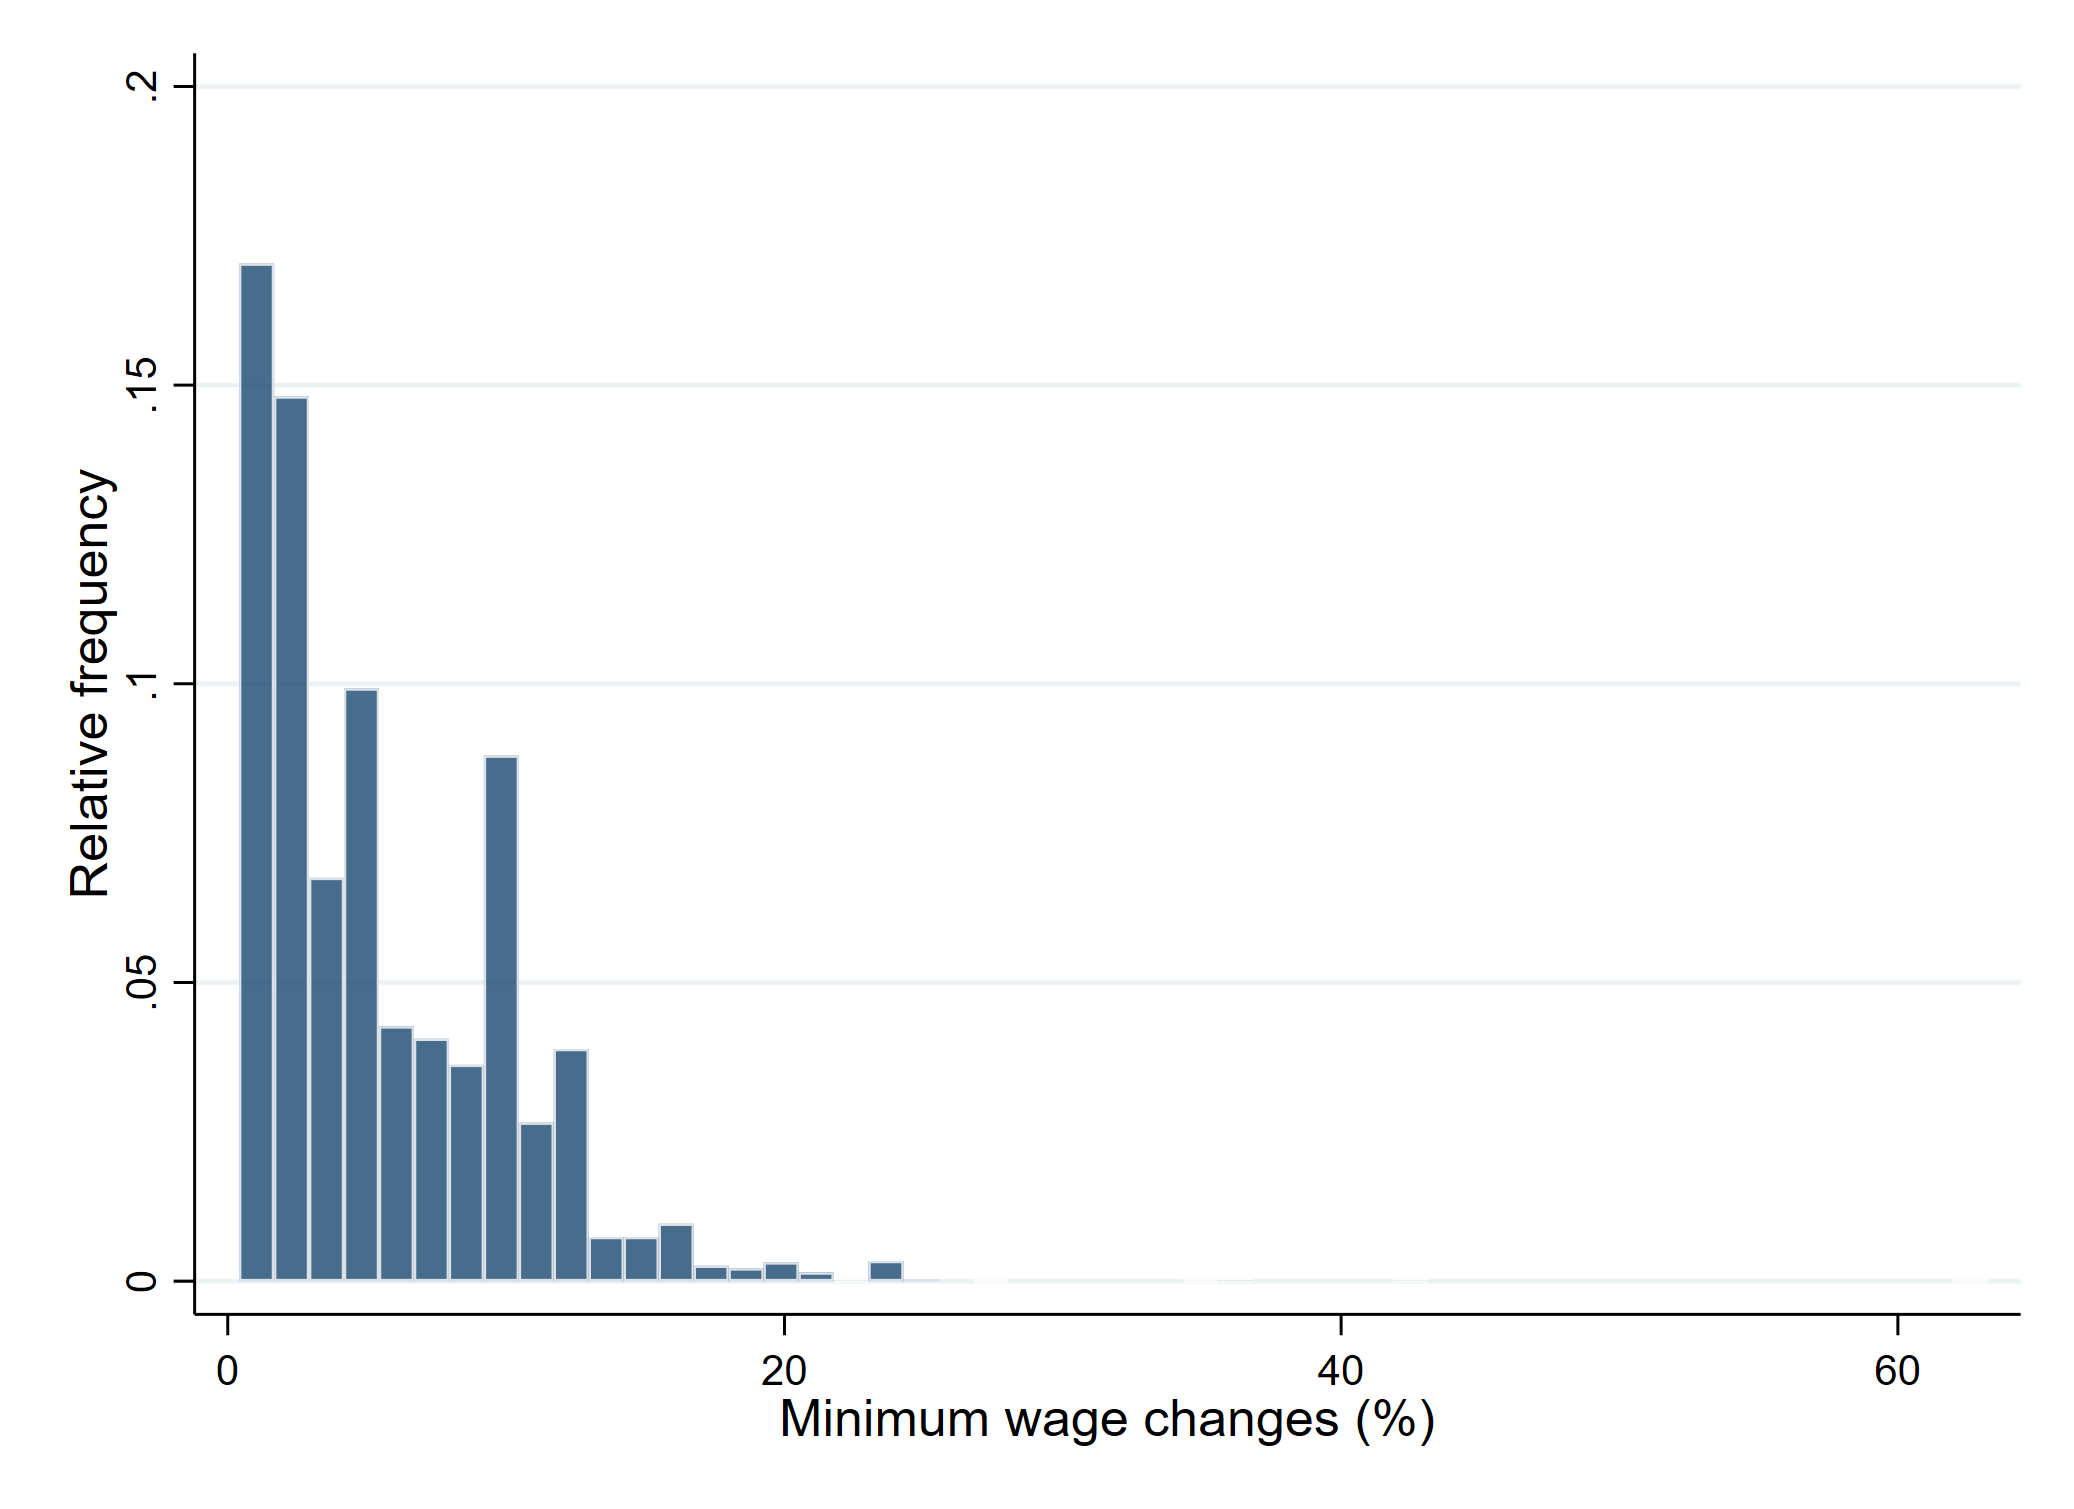
\includegraphics[width = 0.99\textwidth]{descriptive/estimation_samples/output/pct_ch_mw_dist.png}
		\end{subfigure}
	\end{figure}
	
	\hyperlink{stat_MW}{\beamerbutton{Go Back}}
\end{frame}

\begin{frame}[label = dynamic_mw]
	\frametitle{Including leads and lags of residence MW}
	\begin{figure}[h!]
	\centering
		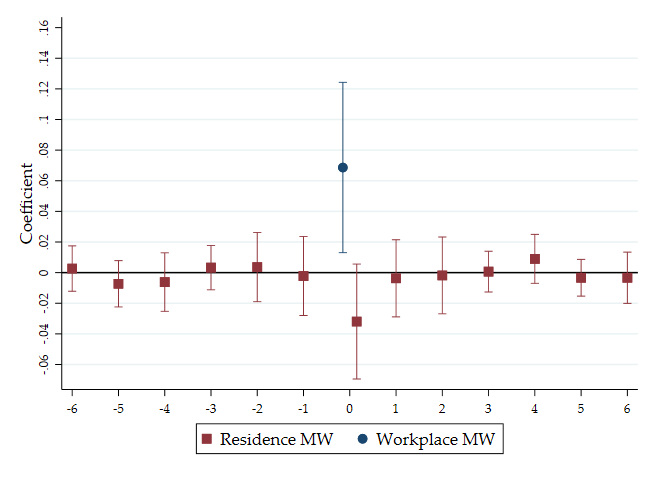
\includegraphics[width=0.7\textwidth]{fd_baseline/output/fd_both_ln_mw_dynamic.png}
	\end{figure}
	\hyperlink{dyn_baseline_plot}{\beamerbutton{Go Back}}
\end{frame}

\begin{frame}[label = fd_both_dynamic]
	\frametitle{Including leads and lags of workplace and residence MW}
	\begin{figure}[h!]
	\centering
		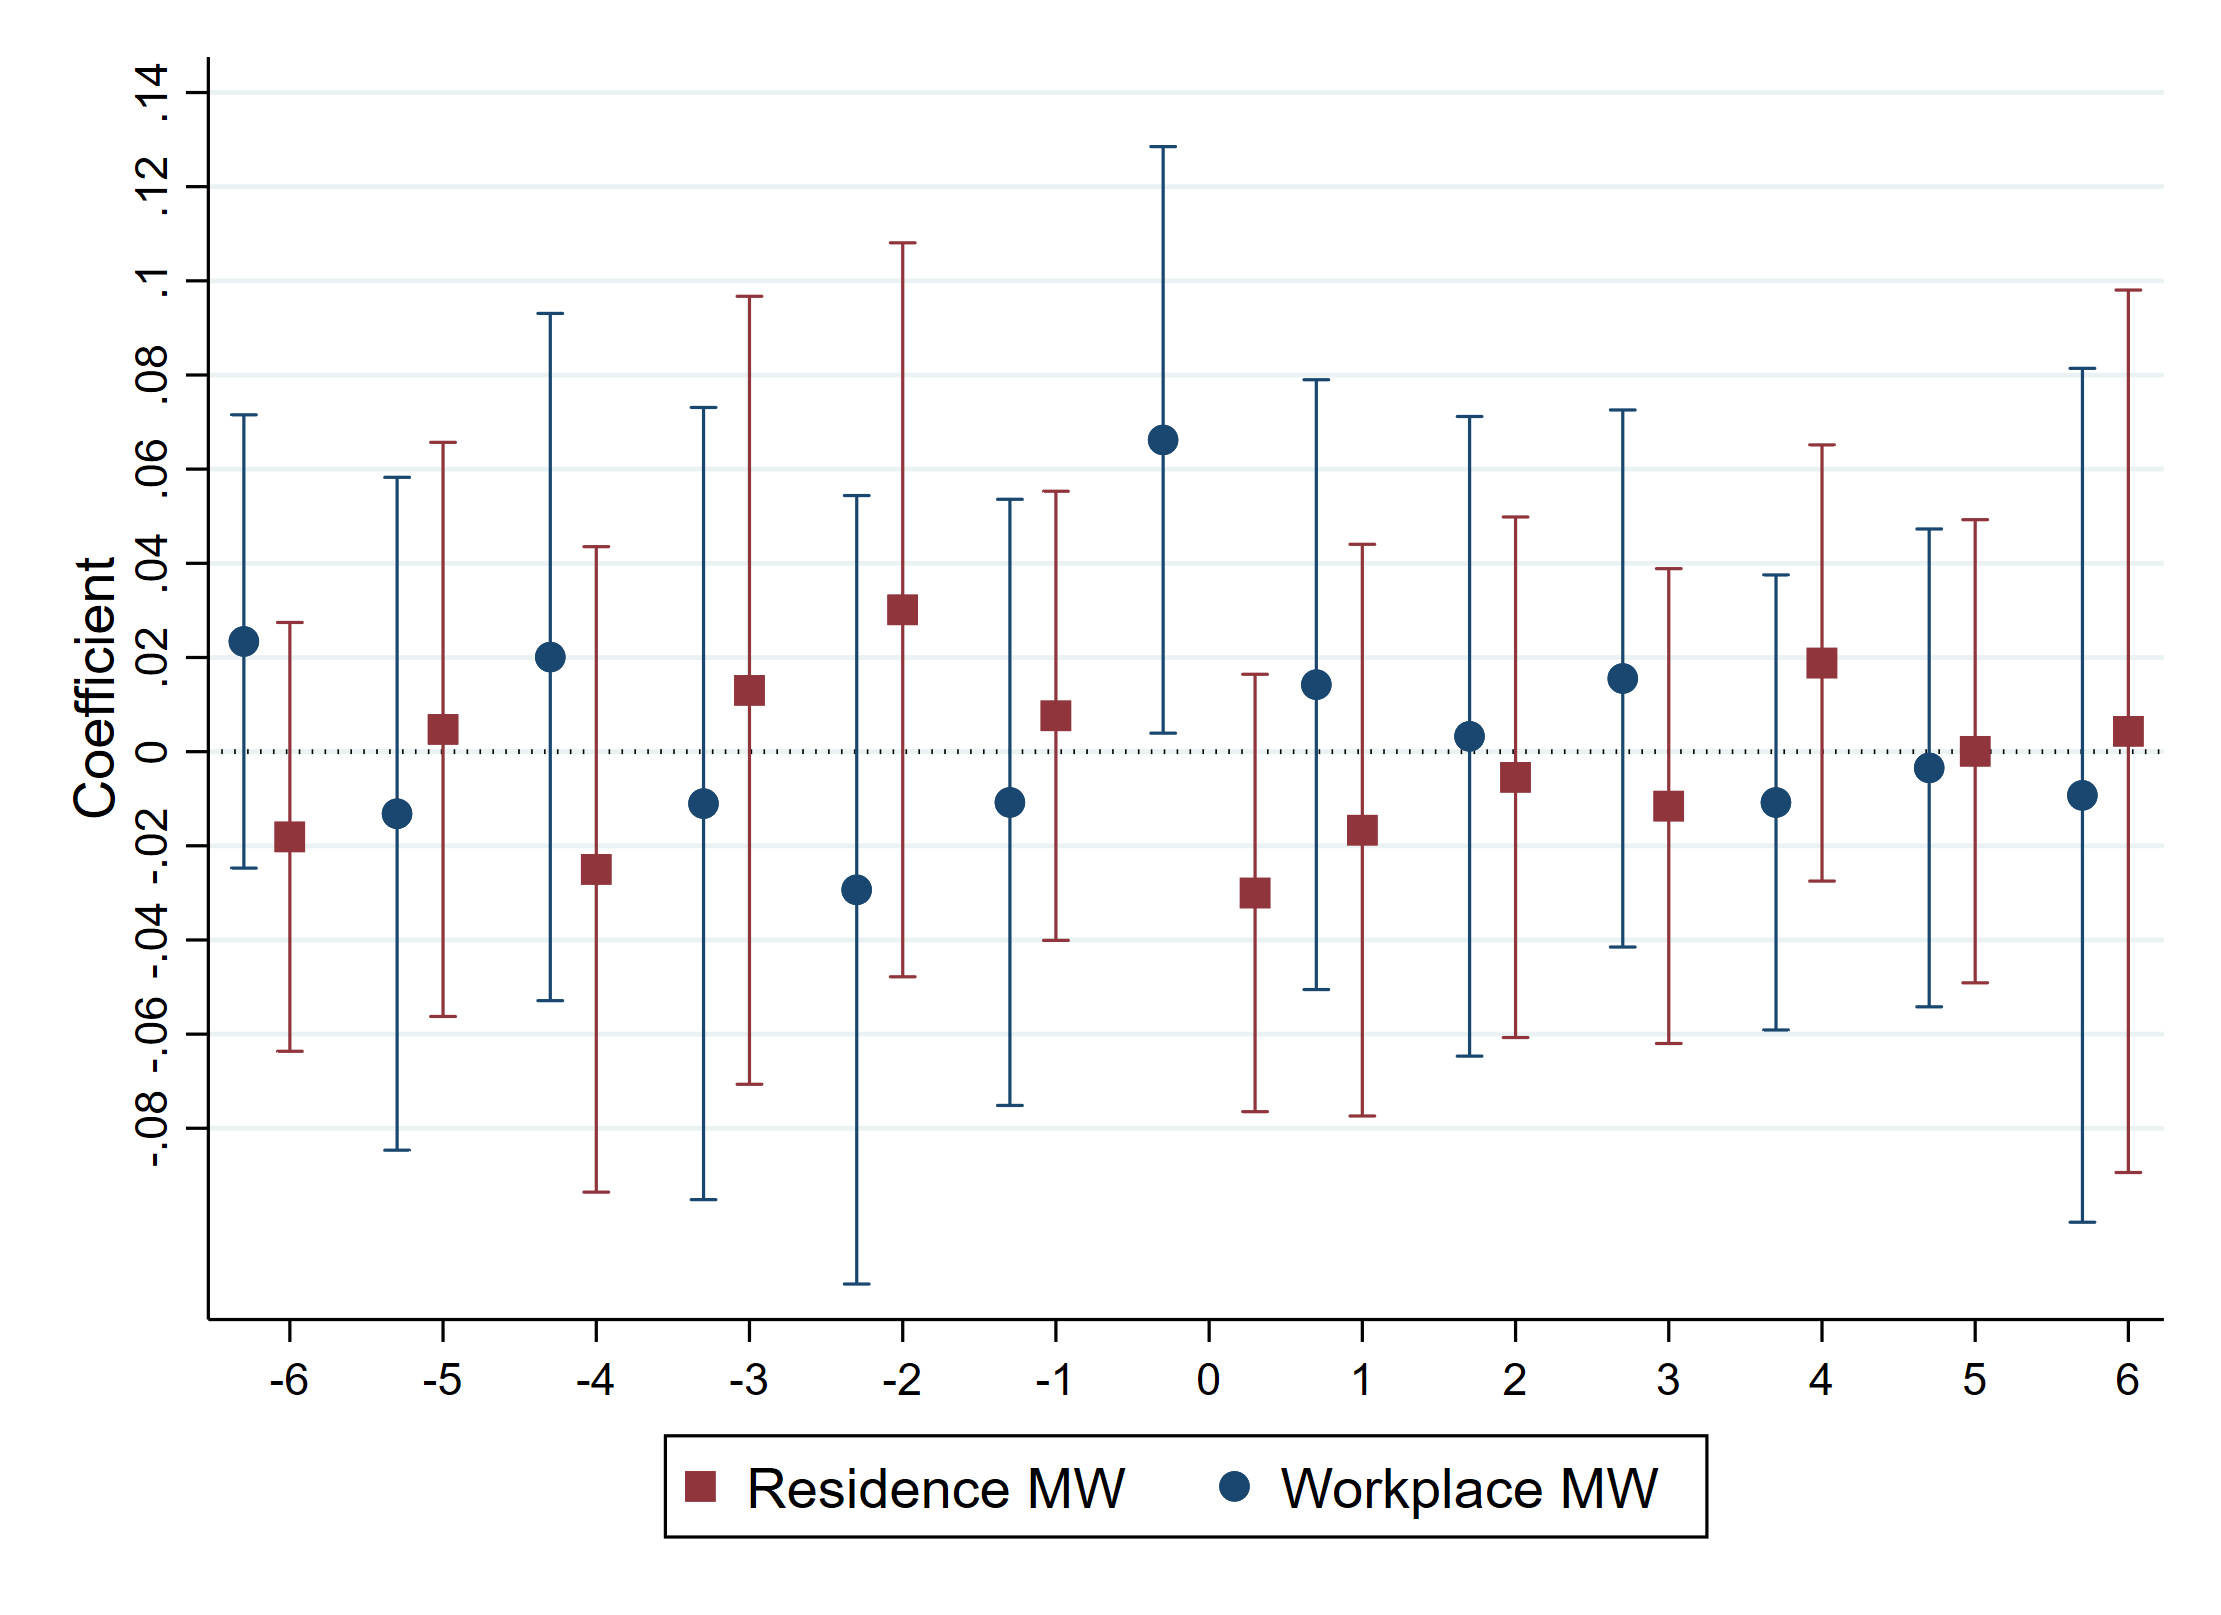
\includegraphics[width=0.7\textwidth]{fd_baseline/output/fd_both_dynamic}
	\end{figure}
	\hyperlink{dyn_baseline_plot}{\beamerbutton{Go Back}}
\end{frame}

\begin{frame}[label = robustness_geo]
	\frametitle{Robustness to geographical trends}
	
	\begin{table}
    \label{tab:static_robust}
    \centering
    \scalebox{0.65}{
    \begin{tabular}{@{}lcccccc@{}}
        \toprule
                                                  & \multicolumn{6}{c}{Change log rents}                                          \\ \cmidrule(l){2-7}
                                                  & \shortstack{Baseline\\(1)}       & \shortstack{No controls\\(2)} & \shortstack{ZIP code trend\\(3)} 
                                                  & \shortstack{County-time FE\\(4)} & \shortstack{CBSA-time FE\\(5)} & \shortstack{State-time FE\\(6)} \\ \midrule
        Change residence minimum wage             & -0.0302      & -0.0289         & -0.0300       & -0.0521        & -0.0596       & -0.0052             \\
                                                  & (0.0169)    & (0.0171)       & (0.0150)     & (0.0346)      & (0.0239)     & (0.0147)           \\
        Change workplace minimum wage             & 0.0645      & 0.0632         & 0.0644       & 0.1231        & 0.1336       & 0.0046             \\
                                                  & (0.0274)    & (0.0279)       & (0.0257)     & (0.0561)      & (0.0498)     & (0.0288)           \\ \midrule
        County-quarter economic controls          & Yes      & No        & Yes       & Yes      & Yes      & Yes              \\
        P-value equality                          & 0.0332      & 0.0407         & 0.0218       & 0.0135        & 0.0117       & 0.8138             \\
        R-squared                                 & 0.0209      & 0.0208         & 0.0228       & 0.1760        & 0.1138       & 0.0605             \\
        Observations                              & 131,196     & 132,255        & 131,196      & 121,928       & 127,079      & 130,656            \\ \bottomrule
    \end{tabular}
    }

\end{table}

	
	\hyperlink{robus_sample}{\beamerbutton{Go Back}}
\end{frame}

\begin{frame}[label = robustness_sample]
	\frametitle{Robustness to different samples}
	
	\begin{table}
    \label{tab:static_sample}
    \scalebox{0.65}{
    \begin{tabular}{@{}lcccccc@{}}
        \toprule
                                           & \multicolumn{6}{c}{Change log rents}                                     \\ \cmidrule(l){2-7} 
                                           & \shortstack{Baseline\\(1)}       & \shortstack{Baseline\\Reweighted (2)}
                                           & \shortstack{Unbalanced\\(3)}     & \shortstack{Unbalanced\\Reweighted (4)}
                                           & \shortstack{Fully-balanced\\(5)} & \shortstack{Fully-balanced\\Reweighted (6)}  \\ \midrule
        Change residence minimum wage      & -0.0204      & -0.0077        & -0.0240       & -0.0163      & -0.0194     & 0.0032            \\
                                           & (0.0169)    & (0.0177)      & (0.0200)     & (0.0192)    & (0.0198)   & (0.0158)          \\
        Change workplace minimum wage      & 0.0545      & 0.0466        & 0.0461       & 0.0376      & 0.0678     & 0.0493            \\
                                           & (0.0283)    & (0.0303)      & (0.0305)     & (0.0343)    & (0.0308)   & (0.0293)          \\ \midrule
        P-value equality                   & 0.0965      & 0.2500        & 0.1586       & 0.3048      & 0.0826     & 0.2983            \\
        R-squared                          & 0.0209      & 0.0205        & 0.0160       & 0.0146      & 0.0216     & 0.0205            \\
        Observations                       & 131,383     & 125,502       & 193,292      & 185,198     & 78,912    & 75,447           \\ \bottomrule
    \end{tabular}
    }
\end{table}

	
	\hyperlink{robus_sample}{\beamerbutton{Go Back}}
\end{frame}

\begin{frame}[label = robustness_exp_mw]
	\frametitle{Robustness to defintion of workplace MW}
	
	\begin{table}
    \label{tab:static_expMW_sensitivity}
    \centering

    \scalebox{0.7}{
    \begin{tabular}{@{}lccccc@{}}
        \toprule
                                                     & \multicolumn{5}{c}{Change log rents}                               \\ \cmidrule(l){2-6}
                                                     & (1)       & (2)        & (3)        &  (4)        & (5)            \\ \midrule
        Change residence minimum wage             & #4#      & #4#         & #4#       & #4#        & #4#                 \\
                                                  & (#4#)    & (#4#)       & (#4#)     & (#4#)      & (#4#)               \\
        Change workplace minimum wage             & #4#      & #4#         & #4#       & #4#        & #4#                 \\
                                                  & (#4#)    & (#4#)       & (#4#)     & (#4#)      & (#4#)               \\
        Commuting shares                           & 2010     &  2014       & 2018    & 2014, low.\ Inc.\    & 2014, young    \\
        P-value equality                          & #4#      & #4#         & #4#       & #4#        & #4#                 \\
        R-squared                                 & #4#      & #4#         & #4#       & #4#        & #4#                 \\
        Observations                              & #0,#     & #0,#        & #0,#      & #0,#       & #0,#               \\ \bottomrule
    \end{tabular}
    }
    
\end{table}

	
	\hyperlink{robus_sample}{\beamerbutton{Go Back}}
\end{frame}

\begin{frame}[label = microfound]
	\frametitle{Microfoundation}
	Say a representative $(i,z)$ worker chooses between housing demand $h_{iz}$,
	non-tradable consumption $c^{\text{NT}}_{iz}$, and tradable consumption $c^{\text{T}}_{iz}$,
	by maximizing
	\[
	u_{iz} = u \left(h_{iz}, c^{\text{NT}}_{iz}, c^{\text{T}}_{iz}\right)
	\]
	subject to

	\[
	r_i h_{iz} + p_i(\MW_i) c^{\text{NT}}_{iz} + c^{\text{T}}_{iz} \leq y_{iz}(\MW_z)
	\]

	where 
	\begin{itemize}
		\item $p_i(\MW_i)$ gives the price of local consumption, increasing in residence MW;
		\item the price of tradable consumption is normalized to one;  
		\item $y_{iz}(\MW_z)$ is an income function that depends positively on the workplace MW.
	\end{itemize}
\end{frame}

\begin{frame}
	\frametitle{Microfoundation (continuation)}

	Let $h_{iz}^*$ and $c_{iz}^*$ denote Marshallian demands, and 
	$\tilde h_{iz}^*$ denote the Hicksian housing demand.

	\vspace{2mm}

	By assumption, the price of the MW will increase prices of non-tradable consumption.
	Thus, consider the effect of an increase in $p_i$ on housing demand.
	The Slutsky equation implies that
	\[
	\frac{\partial h_{iz}^*}{\partial p_i} 
	= \frac{\partial \tilde h_{iz}^*}{\partial p_i} 
	- \frac{\partial h_{iz}^*}{\partial y_{iz}} c_{iz}^*
	\]

	Then, we have that 
	\[
	\frac{\partial h_{iz}^*}{\partial p_i} < 0 \iff 
	\frac{\partial \tilde h_{iz}^*}{\partial p_i} 
	< \frac{\partial h_{iz}^*}{\partial y_{iz}} c_{iz}^*
	\]

	\hyperlink{discuss4}{\beamerbutton{Go Back}}
\end{frame}

\begin{frame}[label = example_pred_chi_07_2019]
	\frametitle{Example Predictions: MMW change in Chicago July 2019}
	
	\begin{figure}
		\begin{subfigure}{0.33\textwidth}
			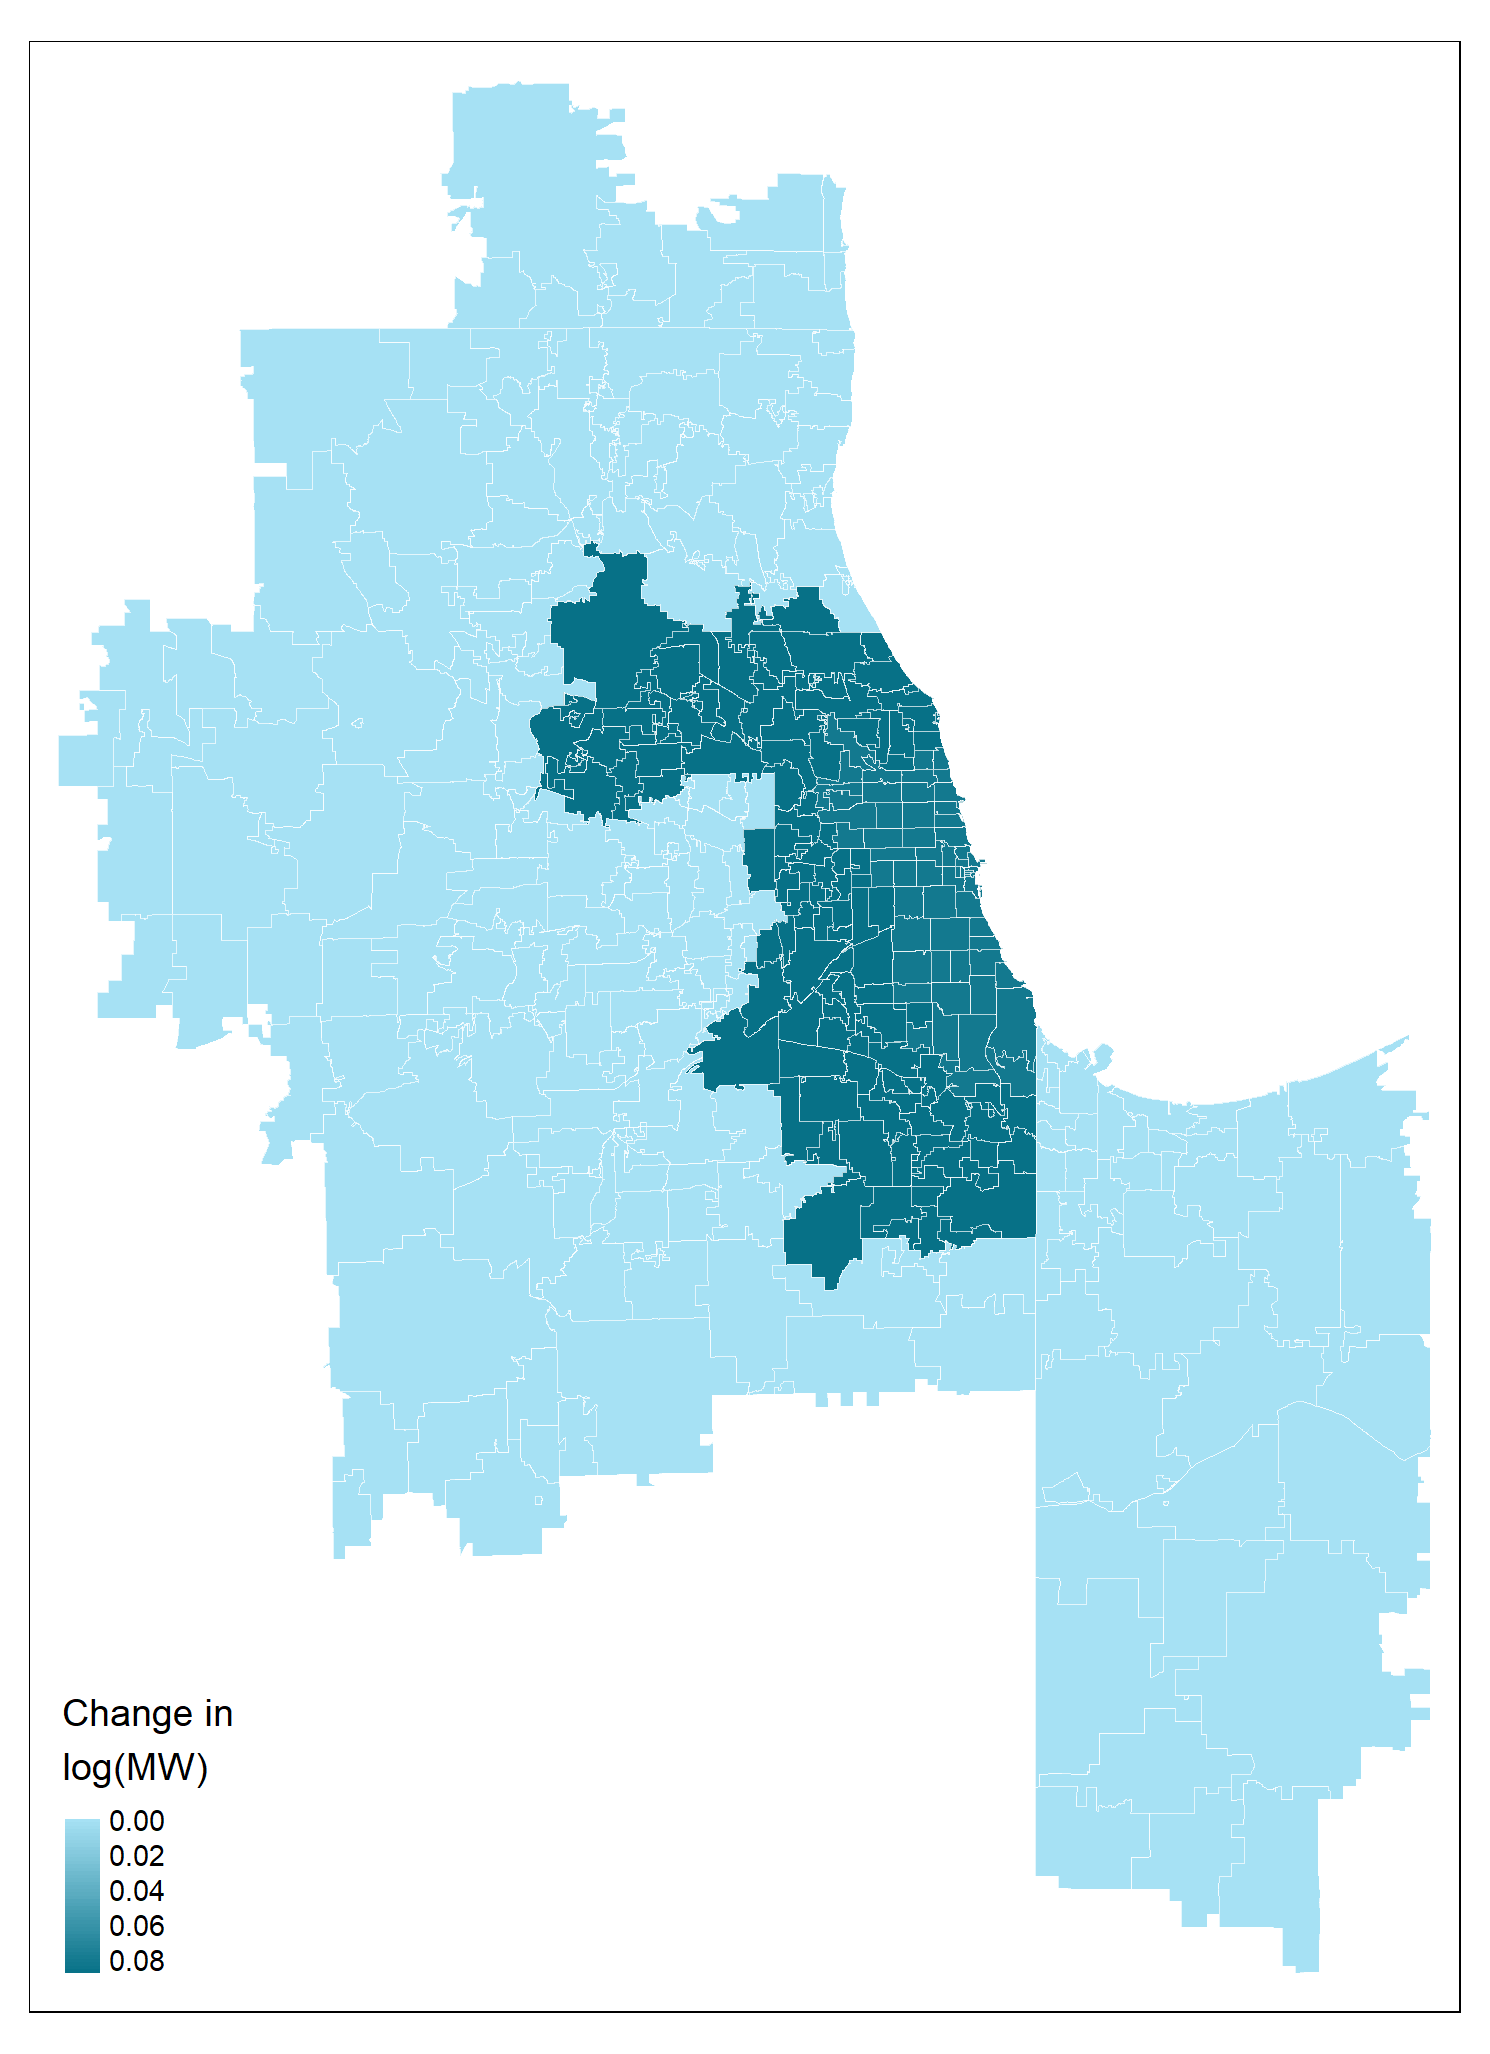
\includegraphics[width = 0.99\textwidth]{maps_events/output/chicago_2019-6_actual_mw.png}
			\caption*{Change in residence MW}
		\end{subfigure}%
		\begin{subfigure}{0.33\textwidth}
                         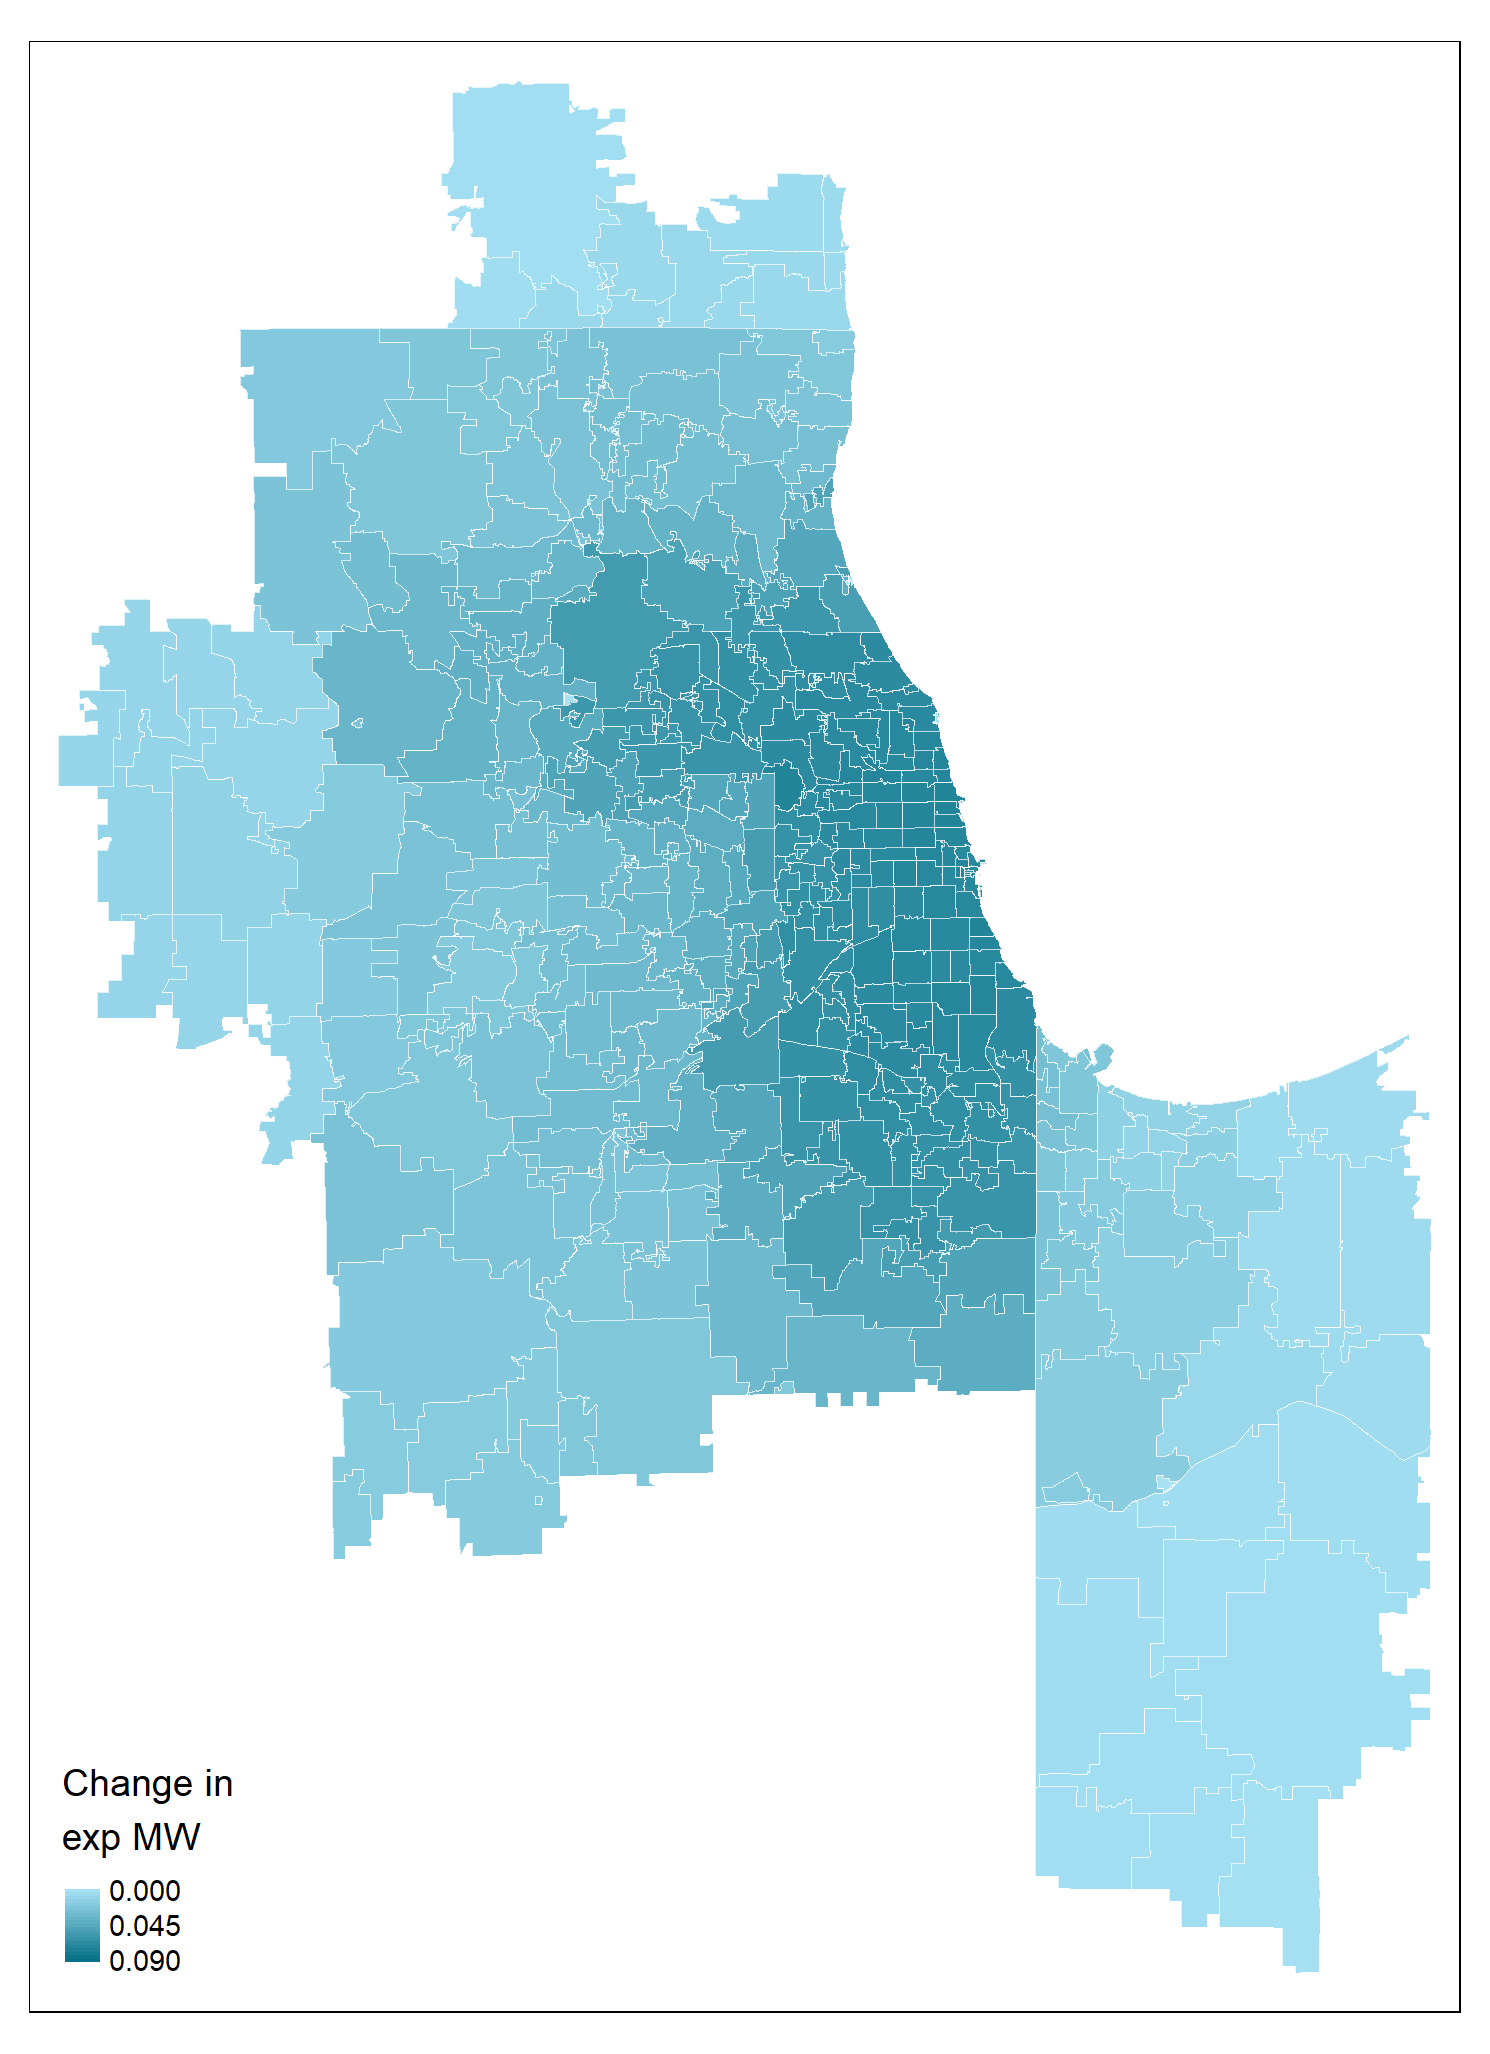
\includegraphics[width = 0.99\textwidth]{maps_events/output/chicago2019-6_exp_mw.png}
			\caption*{Change in workplace MW}
		\end{subfigure}
		\begin{subfigure}{0.33\textwidth}
                         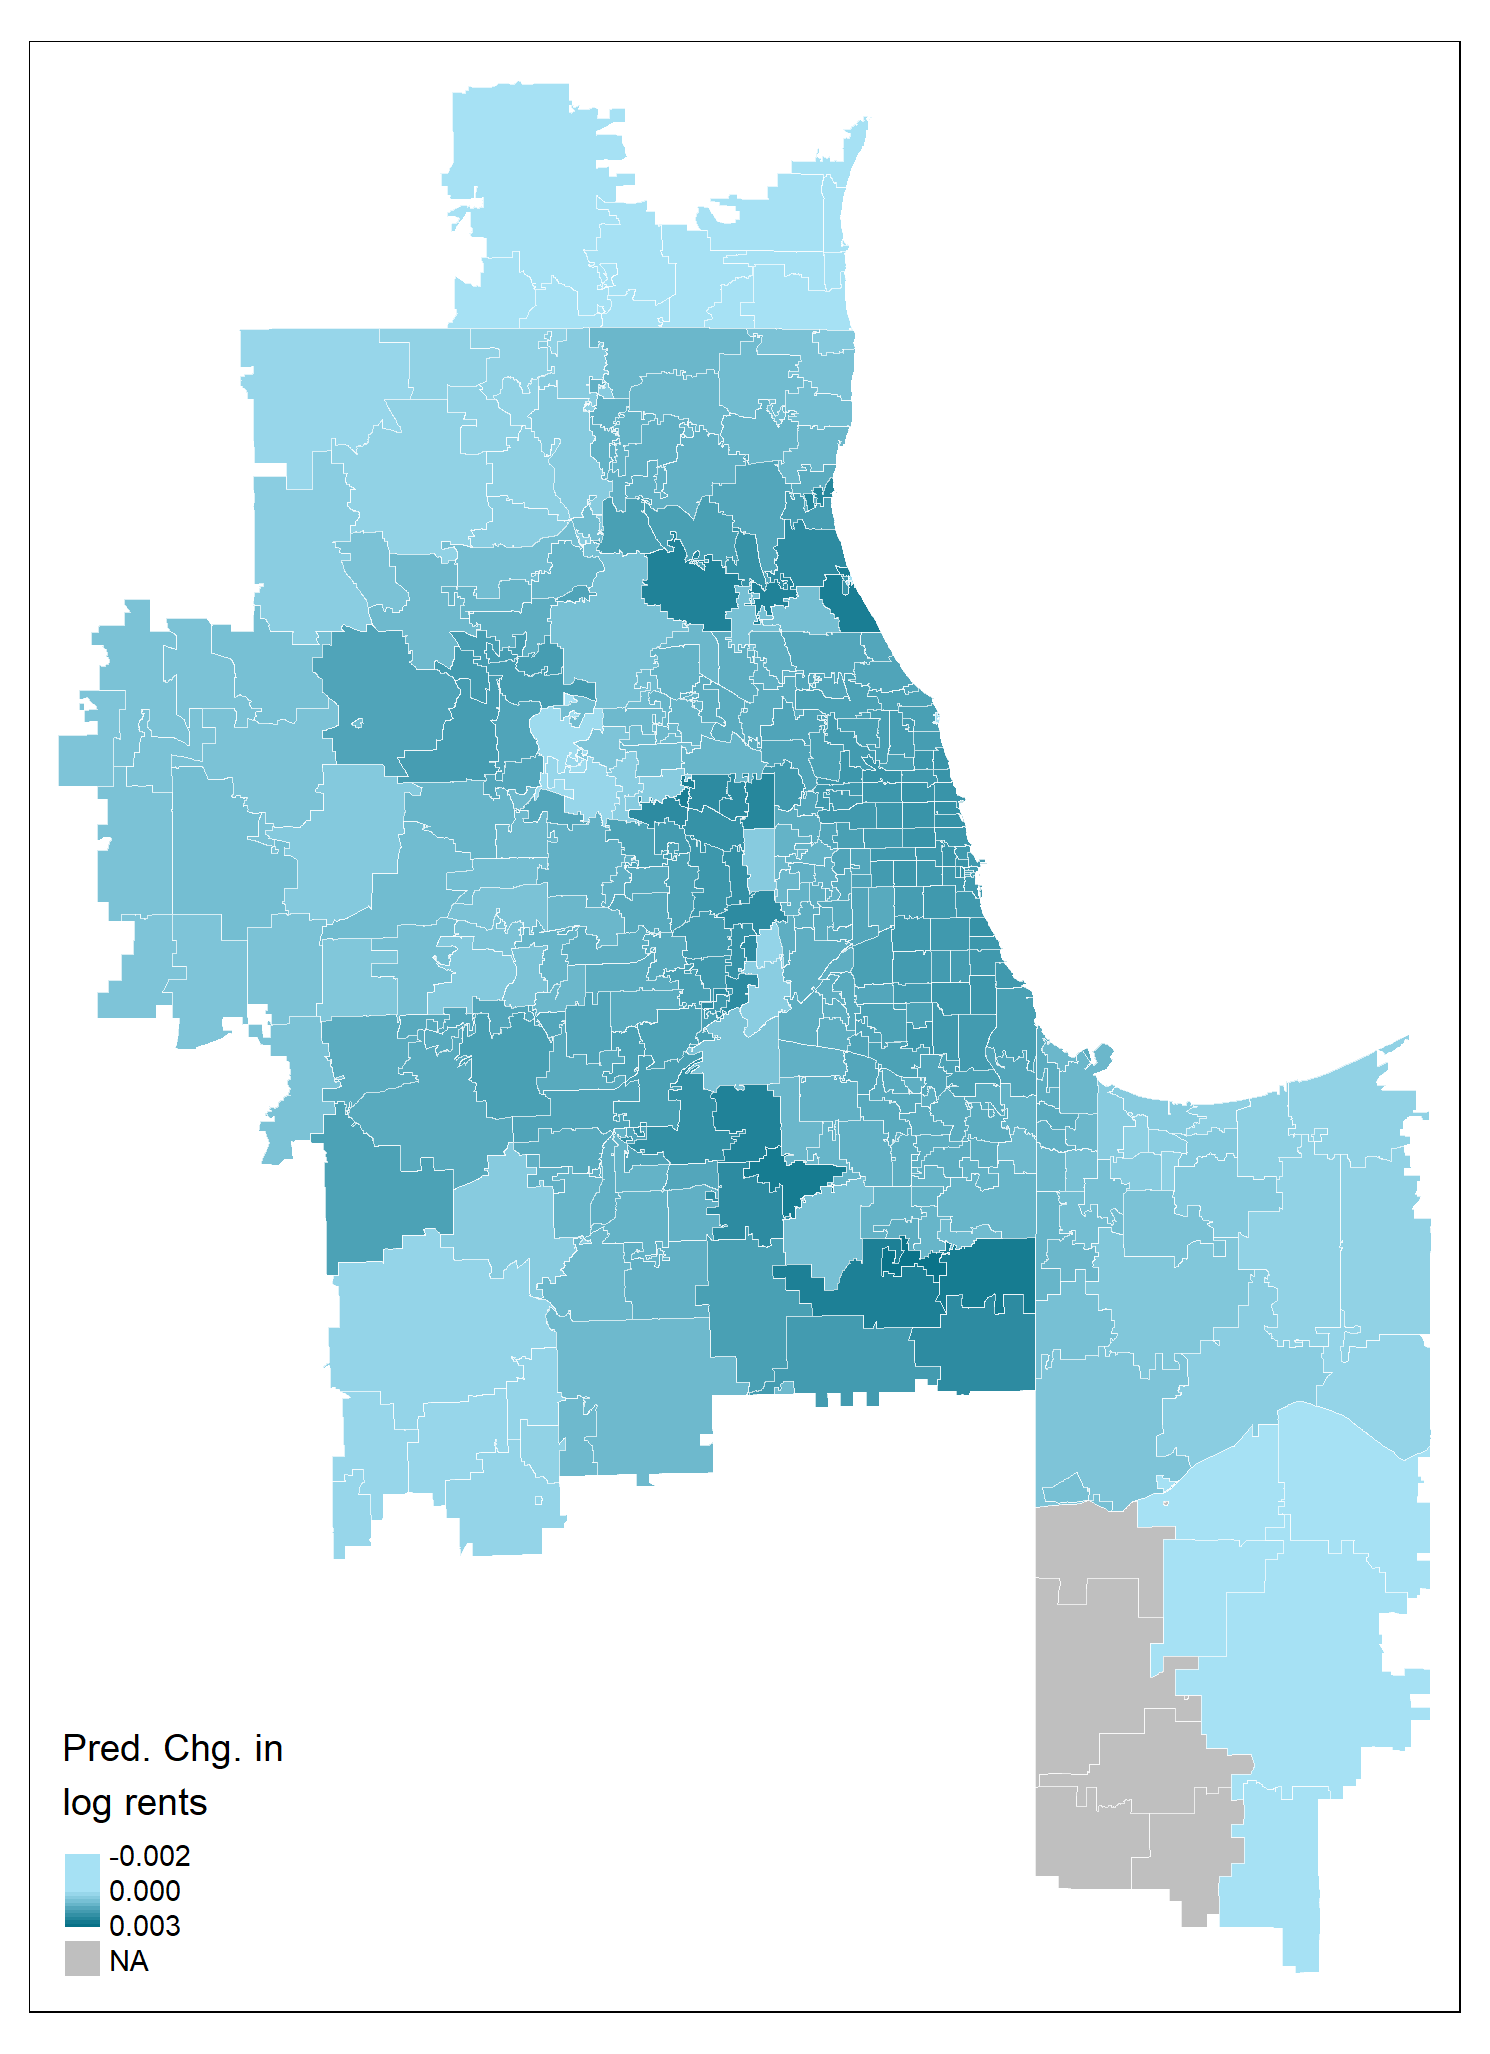
\includegraphics[width = 0.99\textwidth]{prediction_events/output/chicago_2019-7_hatfe_d_ln_rents_baseline.png}
			\caption*{Predicted change in log rents}
		\end{subfigure}
	\end{figure}
	
	\hyperlink{static_tab}{\beamerbutton{Go Back}}
\end{frame}


\end{document}